%&preformat-disser
\RequirePackage[l2tabu,orthodox]{nag} % Раскомментировав, можно в логе получать рекомендации относительно правильного использования пакетов и предупреждения об устаревших и нерекомендуемых пакетах
% Формат А4, 14pt (ГОСТ Р 7.0.11-2011, 5.3.6)
\documentclass[a4paper,14pt,oneside,openany]{memoir}

%%%%%%%%%%%%%%%%%%%%%%%%%%%%%%%%%%%%%%%%%%%%%%%%%%%%%%%%%%%%%%%%%%%%%%%%%%%%%%%%
%%%% Файл упрощённых настроек шаблона, общих для диссертации и автореферата %%%%
%%%%%%%%%%%%%%%%%%%%%%%%%%%%%%%%%%%%%%%%%%%%%%%%%%%%%%%%%%%%%%%%%%%%%%%%%%%%%%%%

%%% Режим черновика %%%
\makeatletter
\@ifundefined{c@draft}{
  \newcounter{draft}
  \setcounter{draft}{0}  % 0 --- чистовик (максимальное соблюдение ГОСТ)
                         % 1 --- черновик (отклонения от ГОСТ, но быстрая
                         %       сборка итоговых PDF)
}{}
\makeatother

%%% Пометки в тексте %%%
\makeatletter
\@ifundefined{c@showmarkup}{
  \newcounter{showmarkup}
  \setcounter{showmarkup}{0}  % 0 --- скрыть пометки
                              % 1 --- показывать пометки
}{}
\makeatother

%%% Использование в pdflatex шрифтов не по-умолчанию %%%
\makeatletter
\@ifundefined{c@usealtfont}{
  \newcounter{usealtfont}
  \setcounter{usealtfont}{1}    % 0 --- шрифты на базе Computer Modern
                                % 1 --- использовать пакет pscyr, при его
                                %       наличии
                                % 2 --- использовать пакет XCharter, при наличии
                                %       подходящей версии
}{}
\makeatother

%%% Использование в xelatex и lualatex семейств шрифтов %%%
\makeatletter
\@ifundefined{c@fontfamily}{
  \newcounter{fontfamily}
  \setcounter{fontfamily}{1}  % 0 --- CMU семейство. Используется как fallback;
                              % 1 --- Шрифты от MS (Times New Roman и компания)
                              % 2 --- Семейство Liberation
}{}
\makeatother

%%% Библиография %%%
\makeatletter
\@ifundefined{c@bibliosel}{
  \newcounter{bibliosel}
  \setcounter{bibliosel}{1}   % 0 --- встроенная реализация с загрузкой файла
                              %       через движок bibtex8;
                              % 1 --- реализация пакетом biblatex через движок
                              %       biber
}{}
\makeatother

%%% Вывод типов ссылок в библиографии %%%
\makeatletter
\@ifundefined{c@mediadisplay}{
  \newcounter{mediadisplay}
  \setcounter{mediadisplay}{1}   % 0 --- не делать ничего; надписи [Текст] и
                                 %       [Эл. ресурс] будут выводиться только в ссылках с
                                 %       заполненным полем `media`;
                                 % 1 --- автоматически добавлять надпись [Текст] к ссылкам с
                                 %       незаполненным полем `media`; таким образом, у всех
                                 %       источников будет указан тип, что соответствует
                                 %       требованиям ГОСТ
                                 % 2 --- автоматически удалять надписи [Текст], [Эл. Ресурс] и др.;
                                 %       не соответствует ГОСТ
                                 % 3 --- автоматически удалять надпись [Текст];
                                 %       не соответствует ГОСТ
                                 % 4 --- автоматически удалять надпись [Эл. Ресурс];
                                 %       не соответствует ГОСТ
}{}
\makeatother

%%% Предкомпиляция tikz рисунков для ускорения работы %%%
\makeatletter
\@ifundefined{c@imgprecompile}{
  \newcounter{imgprecompile}
  \setcounter{imgprecompile}{0}   % 0 --- без предкомпиляции;
                                  % 1 --- пользоваться предварительно
                                  %       скомпилированными pdf вместо генерации
                                  %       заново из tikz
}{}
\makeatother
            % общие настройки шаблона
%%% Проверка используемого TeX-движка %%%
\newif\ifxetexorluatex   % определяем новый условный оператор (http://tex.stackexchange.com/a/47579)
\ifxetex
    \xetexorluatextrue
\else
    \ifluatex
        \xetexorluatextrue
    \else
        \xetexorluatexfalse
    \fi
\fi

\newif\ifsynopsis           % Условие, проверяющее, что документ --- автореферат

\usepackage{etoolbox}[2015/08/02]   % Для продвинутой проверки разных условий
\providebool{presentation}

\usepackage{comment}    % Позволяет убирать блоки текста (добавляет
                        % окружение comment и команду \excludecomment)

%%% Поля и разметка страницы %%%
\usepackage{pdflscape}  % Для включения альбомных страниц
\usepackage{geometry}   % Для последующего задания полей

%%% Математические пакеты %%%
\usepackage{amsthm,amsmath,amscd}   % Математические дополнения от AMS
\usepackage{amsfonts,amssymb}       % Математические дополнения от AMS
\usepackage{mathtools}              % Добавляет окружение multlined
\usepackage{xfrac}                  % Красивые дроби
\usepackage[
    locale = DE,
    list-separator       = {;\,},
    list-final-separator = {;\,},
    list-pair-separator  = {;\,},
    list-units           = single,
    range-units          = single,
    range-phrase={\text{\ensuremath{-}}},
    % quotient-mode        = fraction, % красивые дроби могут не соответствовать ГОСТ
    fraction-function    = \sfrac,
    separate-uncertainty,
    ]{siunitx}[=v2]                 % Размерности SI
\sisetup{inter-unit-product = \ensuremath{{}\cdot{}}}

% Кириллица в нумерации subequations
% Для правильной работы требуется выполнение сразу после загрузки пакетов
\patchcmd{\subequations}{\def\theequation{\theparentequation\alph{equation}}}
{\def\theequation{\theparentequation\asbuk{equation}}}
{\typeout{subequations patched}}{\typeout{subequations not patched}}

%%%% Установки для размера шрифта 14 pt %%%%
%% Формирование переменных и констант для сравнения (один раз для всех подключаемых файлов)%%
%% должно располагаться до вызова пакета fontspec или polyglossia, потому что они сбивают его работу
\newlength{\curtextsize}
\newlength{\bigtextsize}
\setlength{\bigtextsize}{13.9pt}

\makeatletter
%\show\f@size    % неплохо для отслеживания, но вызывает стопорение процесса,
                 % если документ компилируется без команды  -interaction=nonstopmode
\setlength{\curtextsize}{\f@size pt}
\makeatother

%%% Кодировки и шрифты %%%
\ifxetexorluatex
    \ifpresentation
        \providecommand*\autodot{} % quick fix for polyglossia 1.50
    \fi
    \PassOptionsToPackage{no-math}{fontspec}    % https://tex.stackexchange.com/a/26295/104425
    \usepackage{polyglossia}[2014/05/21]        % Поддержка многоязычности
                                        % (fontspec подгружается автоматически)
\else
   %%% Решение проблемы копирования текста в буфер кракозябрами
    \ifnumequal{\value{usealtfont}}{0}{}{
        \input glyphtounicode.tex
        \input glyphtounicode-cmr.tex %from pdfx package
        \pdfgentounicode=1
    }
    \usepackage{cmap}   % Улучшенный поиск русских слов в полученном pdf-файле
    \ifnumequal{\value{usealtfont}}{2}{}{
        \defaulthyphenchar=127  % Если стоит до fontenc, то переносы
                                % не впишутся в выделяемый текст при
                                % копировании его в буфер обмена
    }
    \usepackage{textcomp}
    \usepackage[T1,T2A]{fontenc}                    % Поддержка русских букв
    \ifnumequal{\value{usealtfont}}{1}{% Используется pscyr, при наличии
        \IfFileExists{pscyr.sty}{\usepackage{pscyr}}{}  % Подключение pscyr
    }{}
    \usepackage[utf8]{inputenc}[2014/04/30]         % Кодировка utf8
    \usepackage[english, russian]{babel}[2014/03/24]% Языки: русский, английский
    \makeatletter\AtBeginDocument{\let\@elt\relax}\makeatother % babel 3.40 fix
    \ifnumequal{\value{usealtfont}}{2}{
        % http://dxdy.ru/post1238763.html#p1238763
        \usepackage[scaled=0.914]{XCharter}[2017/12/19] % Подключение русифицированных шрифтов XCharter
        \usepackage[charter, vvarbb, scaled=1.048]{newtxmath}[2017/12/14]
        \ifpresentation
        \else
            \setDisplayskipStretch{-0.078}
        \fi
    }{}
\fi

%%% Оформление абзацев %%%
\ifpresentation
\else
    \indentafterchapter     % Красная строка после заголовков типа chapter
    \usepackage{indentfirst}
\fi

%%% Цвета %%%
\ifpresentation
\else
    \usepackage[dvipsnames, table, hyperref]{xcolor} % Совместимо с tikz
\fi

%%% Таблицы %%%
\usepackage{longtable,ltcaption} % Длинные таблицы
\usepackage{multirow,makecell}   % Улучшенное форматирование таблиц
%\usepackage{tabu, tabulary}      % таблицы с автоматически подбирающейся
                                 % шириной столбцов (tabu обязательно
                                 % до hyperref вызывать)
\usepackage{tabu}   
\usepackage{tabulary}                            
\makeatletter
%%https://github.com/tabu-issues-for-future-maintainer/tabu/issues/26
%%\@ifpackagelater{longtable}{2020/02/07}{
\def\tabuendlongtrial{%
    \LT@echunk  \global\setbox\LT@gbox \hbox{\unhbox\LT@gbox}\kern\wd\LT@gbox
                \LT@get@widths
}%
\makeatother

\usepackage{threeparttable}      % автоматический подгон ширины подписи таблицы

%%% Общее форматирование
\usepackage{soulutf8}% Поддержка переносоустойчивых подчёркиваний и зачёркиваний
\usepackage{icomma}  % Запятая в десятичных дробях

%%% Оптимизация расстановки переносов и длины последней строки абзаца
\IfFileExists{impnattypo.sty}{% проверка установленности пакета impnattypo
    \ifluatex
        \ifnumequal{\value{draft}}{1}{% Черновик
            \usepackage[hyphenation, lastparline, nosingleletter, homeoarchy,
            rivers, draft]{impnattypo}
        }{% Чистовик
            \usepackage[hyphenation, lastparline, nosingleletter]{impnattypo}
        }
    \else
        \usepackage[hyphenation, lastparline]{impnattypo}
    \fi
}{}

%% Векторная графика

\usepackage{tikz}                   % Продвинутый пакет векторной графики
\usetikzlibrary{chains}             % Для примера tikz рисунка
\usetikzlibrary{shapes.geometric}   % Для примера tikz рисунка
\usetikzlibrary{shapes.symbols}     % Для примера tikz рисунка
\usetikzlibrary{arrows}             % Для примера tikz рисунка

%%% Гиперссылки %%%
\ifxetexorluatex
    \let\CYRDZE\relax
\fi
\usepackage{hyperref}[2012/11/06]

%%% Изображения %%%
\usepackage{graphicx}[2014/04/25]   % Подключаем пакет работы с графикой
\usepackage{caption}                % Подписи рисунков и таблиц
\usepackage{subcaption}             % Подписи подрисунков и подтаблиц
\usepackage{pdfpages}               % Добавление внешних pdf файлов

%%% Счётчики %%%
\usepackage{aliascnt}
\usepackage[figure,table]{totalcount}   % Счётчик рисунков и таблиц
\usepackage{totcount}   % Пакет создания счётчиков на основе последнего номера
                        % подсчитываемого элемента (может требовать дважды
                        % компилировать документ)
\usepackage{totpages}   % Счётчик страниц, совместимый с hyperref (ссылается
                        % на номер последней страницы). Желательно ставить
                        % последним пакетом в преамбуле

%%% Продвинутое управление групповыми ссылками (пока только формулами) %%%
\ifpresentation
\else
    \usepackage[russian]{cleveref} % cleveref имеет сложности со считыванием
    % языка из babel. Такое решение русификации вывода выбрано вместо
    % определения в documentclass из опасности что-то лишнее передать во все
    % остальные пакеты, включая библиографию.

    % Добавление возможности использования пробелов в \labelcref
    % https://tex.stackexchange.com/a/340502/104425
    \usepackage{kvsetkeys}
    \makeatletter
    \let\org@@cref\@cref
    \renewcommand*{\@cref}[2]{%
        \edef\process@me{%
            \noexpand\org@@cref{#1}{\zap@space#2 \@empty}%
        }\process@me
    }
    \makeatother
\fi

\usepackage{placeins} % для \FloatBarrier

\ifnumequal{\value{draft}}{1}{% Черновик
    \usepackage[firstpage]{draftwatermark}
    \SetWatermarkText{DRAFT}
    \SetWatermarkFontSize{14pt}
    \SetWatermarkScale{15}
    \SetWatermarkAngle{45}
}{}

%%% Цитата, не приводимая в автореферате:
% возможно, актуальна только для biblatex
%\newcommand{\citeinsynopsis}[1]{\ifsynopsis\else ~\cite{#1} \fi}

% если текущий процесс запущен библиотекой tikz-external, то прекомпиляция должна быть включена
\ifdefined\tikzexternalrealjob
    \setcounter{imgprecompile}{1}
\fi

\ifnumequal{\value{imgprecompile}}{1}{% Только если у нас включена предкомпиляция
    \usetikzlibrary{external}   % подключение возможности предкомпиляции
    \tikzexternalize[prefix=images/cache/,optimize command away=\includepdf] % activate! % здесь можно указать отдельную папку для скомпилированных файлов
    \ifxetex
        \tikzset{external/up to date check={diff}}
    \fi
}{}
         % Пакеты общие для диссертации и автореферата
\synopsisfalse                      % Этот документ --- не автореферат
%%% Прикладные пакеты %%%
%\usepackage{calc}               % Пакет для расчётов параметров, например длины

%%% Для добавления Стр. над номерами страниц в оглавлении
%%% http://tex.stackexchange.com/a/306950
\usepackage{afterpage}

%%% Списки %%%
\usepackage{enumitem}

%%% Оформление списка обозначений
%\usepackage[intoc]{nomencl}
\usepackage{nomencl}
\makenomenclature
\setlength{\nomitemsep}{-.8\parsep}
    % Пакеты для диссертации
\input{Dissertation/userpackages}   % Пакеты для специфических пользовательских задач

%%%%%%%%%%%%%%%%%%%%%%%%%%%%%%%%%%%%%%%%%%%%%%%%%%%%%%
%%%% Файл упрощённых настроек шаблона диссертации %%%%
%%%%%%%%%%%%%%%%%%%%%%%%%%%%%%%%%%%%%%%%%%%%%%%%%%%%%%

%%% Инициализирование переменных, не трогать!  %%%
\newcounter{intvl}
\newcounter{otstup}
\newcounter{contnumeq}
\newcounter{contnumfig}
\newcounter{contnumtab}
\newcounter{pgnum}
\newcounter{chapstyle}
\newcounter{headingdelim}
\newcounter{headingalign}
\newcounter{headingsize}
%%%%%%%%%%%%%%%%%%%%%%%%%%%%%%%%%%%%%%%%%%%%%%%%%%%%%%

%%% Область упрощённого управления оформлением %%%

%% Интервал между заголовками и между заголовком и текстом %%
% Заголовки отделяют от текста сверху и снизу
% тремя интервалами (ГОСТ Р 7.0.11-2011, 5.3.5)
\setcounter{intvl}{3}               % Коэффициент кратности к размеру шрифта

%% Отступы у заголовков в тексте %%
\setcounter{otstup}{0}              % 0 --- без отступа; 1 --- абзацный отступ

%% Нумерация формул, таблиц и рисунков %%
% Нумерация формул
\setcounter{contnumeq}{0}   % 0 --- пораздельно (во введении подряд,
                            %       без номера раздела);
                            % 1 --- сквозная нумерация по всей диссертации
% Нумерация рисунков
\setcounter{contnumfig}{0}  % 0 --- пораздельно (во введении подряд,
                            %       без номера раздела);
                            % 1 --- сквозная нумерация по всей диссертации
% Нумерация таблиц
\setcounter{contnumtab}{0}  % 0 --- пораздельно (во введении подряд,
                            %       без номера раздела);
                            % 1 --- сквозная нумерация по всей диссертации

%% Оглавление %%
\setcounter{pgnum}{1}       % 0 --- номера страниц никак не обозначены;
                            % 1 --- Стр. над номерами страниц (дважды
                            %       компилировать после изменения настройки)
\settocdepth{subsection}    % до какого уровня подразделов выносить в оглавление
\setsecnumdepth{subsection} % до какого уровня нумеровать подразделы


%% Текст и форматирование заголовков %%
\setcounter{chapstyle}{1}     % 0 --- разделы только под номером;
                              % 1 --- разделы с названием "Глава" перед номером
\setcounter{headingdelim}{1}  % 0 --- номер отделен пропуском в 1em или \quad;
                              % 1 --- номера разделов и приложений отделены
                              %       точкой с пробелом, подразделы пропуском
                              %       без точки;
                              % 2 --- номера разделов, подразделов и приложений
                              %       отделены точкой с пробелом.

%% Выравнивание заголовков в тексте %%
\setcounter{headingalign}{0}  % 0 --- по центру;
                              % 1 --- по левому краю

%% Размеры заголовков в тексте %%
\setcounter{headingsize}{0}   % 0 --- по ГОСТ, все всегда 14 пт;
                              % 1 --- пропорционально изменяющийся размер
                              %       в зависимости от базового шрифта

%% Подпись таблиц %%

% Смещение строк подписи после первой строки
\newcommand{\tabindent}{0cm}

% Тип форматирования заголовка таблицы:
% plain --- название и текст в одной строке
% split --- название и текст в разных строках
\newcommand{\tabformat}{plain}

%%% Настройки форматирования таблицы `plain`

% Выравнивание по центру подписи, состоящей из одной строки:
% true  --- выравнивать
% false --- не выравнивать
\newcommand{\tabsinglecenter}{false}

% Выравнивание подписи таблиц:
% justified   --- выравнивать как обычный текст («по ширине»)
% centering   --- выравнивать по центру
% centerlast  --- выравнивать по центру только последнюю строку
% centerfirst --- выравнивать по центру только первую строку (не рекомендуется)
% raggedleft  --- выравнивать по правому краю
% raggedright --- выравнивать по левому краю
\newcommand{\tabjust}{justified}

% Разделитель записи «Таблица #» и названия таблицы
\newcommand{\tablabelsep}{~\cyrdash\ }

%%% Настройки форматирования таблицы `split`

% Положение названия таблицы:
% \centering   --- выравнивать по центру
% \raggedleft  --- выравнивать по правому краю
% \raggedright --- выравнивать по левому краю
\newcommand{\splitformatlabel}{\raggedleft}

% Положение текста подписи:
% \centering   --- выравнивать по центру
% \raggedleft  --- выравнивать по правому краю
% \raggedright --- выравнивать по левому краю
\newcommand{\splitformattext}{\raggedright}

%% Подпись рисунков %%
%Разделитель записи «Рисунок #» и названия рисунка
\newcommand{\figlabelsep}{~\cyrdash\ }  % (ГОСТ 2.105, 4.3.1)
                                        % "--- здесь не работает

%%% Цвета гиперссылок %%%
% Latex color definitions: http://latexcolor.com/

%было
%\definecolor{linkcolor}{rgb}{0.9,0,0}
%\definecolor{citecolor}{rgb}{0,0.6,0}
%\definecolor{urlcolor}{rgb}{0,0,1}
%стало
\definecolor{linkcolor}{rgb}{0,0,0}
\definecolor{citecolor}{rgb}{0,0,0}
\definecolor{urlcolor}{rgb}{0,0,0}
%\definecolor{linkcolor}{rgb}{0,0,0} %black
%\definecolor{citecolor}{rgb}{0,0,0} %black
%\definecolor{urlcolor}{rgb}{0,0,0} %black
      % Упрощённые настройки шаблона

% Новые переменные, которые могут использоваться во всём проекте
% ГОСТ 7.0.11-2011
% 9.2 Оформление текста автореферата диссертации
% 9.2.1 Общая характеристика работы включает в себя следующие основные структурные
% элементы:
% актуальность темы исследования;
\newcommand{\actualityTXT}{Актуальность темы.}
% степень ее разработанности;
\newcommand{\progressTXT}{Степень разработанности темы.}
% цели и задачи;
\newcommand{\aimTXT}{Целями}
\newcommand{\tasksTXT}{задачи}
% научную новизну;
\newcommand{\noveltyTXT}{Научная новизна:}
% теоретическую и практическую значимость работы;
%\newcommand{\influenceTXT}{Теоретическая и практическая значимость}
% или чаще используют просто
\newcommand{\influenceTXT}{Практическая значимость}
% методологию и методы исследования;
\newcommand{\methodsTXT}{Методология и методы исследования.}
% положения, выносимые на защиту;
\newcommand{\defpositionsTXT}{Основные положения, выносимые на~защиту:}
% степень достоверности и апробацию результатов.
\newcommand{\reliabilityTXT}{Достоверность}
\newcommand{\probationTXT}{Апробация работы.}

\newcommand{\contributionTXT}{Личный вклад.}
\newcommand{\publicationsTXT}{Публикации.}


%%% Заголовки библиографии:

% для автореферата:
\newcommand{\bibtitleauthor}{Публикации автора по теме диссертации}

% для стиля библиографии `\insertbiblioauthorgrouped`
\newcommand{\bibtitleauthorvak}{В изданиях из списка ВАК РФ}
\newcommand{\bibtitleauthorscopus}{В изданиях, входящих в международную базу цитирования Scopus}
\newcommand{\bibtitleauthorwos}{В изданиях, входящих в международную базу цитирования Web of Science}
\newcommand{\bibtitleauthorother}{В прочих изданиях}
\newcommand{\bibtitleauthorconf}{В сборниках трудов конференций}
\newcommand{\bibtitleauthorpatent}{Зарегистрированные патенты}
\newcommand{\bibtitleauthorprogram}{Зарегистрированные программы для ЭВМ}

% для стиля библиографии `\insertbiblioauthorimportant`:
\newcommand{\bibtitleauthorimportant}{Наиболее значимые \protect\MakeLowercase\bibtitleauthor}

% для списка литературы в диссертации и списка чужих работ в автореферате:
\newcommand{\bibtitlefull}{Список литературы} % (ГОСТ Р 7.0.11-2011, 4)
         % Новые переменные, для всего проекта

%%% Основные сведения %%%
\newcommand{\thesisAuthorLastName}{\fixme{Лукьянчук}}
\newcommand{\thesisAuthorOtherNames}{\fixme{Антон Алексеевич}}
\newcommand{\thesisAuthorInitials}{\fixme{И.\,О.}}
\newcommand{\thesisAuthor}             % Диссертация, ФИО автора
{%
    \texorpdfstring{% \texorpdfstring takes two arguments and uses the first for (La)TeX and the second for pdf
        \thesisAuthorLastName~\thesisAuthorOtherNames% так будет отображаться на титульном листе или в тексте, где будет использоваться переменная
    }{%
        \thesisAuthorLastName, \thesisAuthorOtherNames% эта запись для свойств pdf-файла. В таком виде, если pdf будет обработан программами для сбора библиографических сведений, будет правильно представлена фамилия.
    }
}
\newcommand{\thesisAuthorShort}        % Диссертация, ФИО автора инициалами
{\thesisAuthorInitials~\thesisAuthorLastName}
%\newcommand{\thesisUdk}                % Диссертация, УДК
%{\fixme{xxx.xxx}}
\newcommand{\thesisTitle}              % Диссертация, название
{\fixme{РАЗРАБОТКА АТОМНО-ЗОНДОВОГО ТОМОГРАФА С ФЕМТОСЕКУНДНЫМ ЛАЗЕРНЫМ ИСПАРЕНИЕМ ДЛЯ ИЗУЧЕНИЯ ТРЕХМЕРНОГО РАСПРЕДЕЛЕНИЯ ЭЛЕМЕНТОВ С АТОМАРНЫМ МАСШТАБОМ В СТАЛЯХ И СПЛАВАХ}}
\newcommand{\thesisSpecialtyNumber}    % Диссертация, специальность, номер
{\fixme{01.04.01}}
\newcommand{\thesisSpecialtyTitle}     % Диссертация, специальность, название (название взято с сайта ВАК для примера)
{\fixme{Приборы и методы экспериментальной физики}}
%% \newcommand{\thesisSpecialtyTwoNumber} % Диссертация, вторая специальность, номер
%% {\fixme{XX.XX.XX}}
%% \newcommand{\thesisSpecialtyTwoTitle}  % Диссертация, вторая специальность, название
%% {\fixme{Теория и~методика физического воспитания, спортивной тренировки,
%% оздоровительной и~адаптивной физической культуры}}
\newcommand{\thesisDegree}             % Диссертация, ученая степень
{\fixme{кандидата физико-математических наук}}
\newcommand{\thesisDegreeShort}        % Диссертация, ученая степень, краткая запись
{\fixme{канд. физ.-мат. наук}}
\newcommand{\thesisCity}               % Диссертация, город написания диссертации
{\fixme{Москва}}
\newcommand{\thesisYear}               % Диссертация, год написания диссертации
{\the\year}
\newcommand{\thesisOrganization}       % Диссертация, организация
{\fixme{Федеральное государственное бюджетное учреждение
<<Национального исследовательского центра «Курчатовский Институт»}}
\newcommand{\thesisOrganizationShort}  % Диссертация, краткое название организации для доклада
{\fixme{НазУчДисРаб}}

\newcommand{\thesisInOrganization}     % Диссертация, организация в предложном падеже: Работа выполнена в ...
{\fixme{учреждении с~длинным длинным длинным длинным названием, в~котором
выполнялась данная диссертационная работа}}

%% \newcommand{\supervisorDead}{}           % Рисовать рамку вокруг фамилии
\newcommand{\supervisorFio}              % Научный руководитель, ФИО
{\fixme{Рогожкин Сергей Васильевич}}
\newcommand{\supervisorRegalia}          % Научный руководитель, регалии
{\fixme{доктор физико-математических наук}}
\newcommand{\supervisorFioShort}         % Научный руководитель, ФИО
{\fixme{И.\,О.~Фамилия}}
\newcommand{\supervisorRegaliaShort}     % Научный руководитель, регалии
{\fixme{уч.~ст.,~уч.~зв.}}

%% \newcommand{\supervisorTwoDead}{}        % Рисовать рамку вокруг фамилии
%% \newcommand{\supervisorTwoFio}           % Второй научный руководитель, ФИО
%% {\fixme{Фамилия Имя Отчество}}
%% \newcommand{\supervisorTwoRegalia}       % Второй научный руководитель, регалии
%% {\fixme{уч. степень, уч. звание}}
%% \newcommand{\supervisorTwoFioShort}      % Второй научный руководитель, ФИО
%% {\fixme{И.\,О.~Фамилия}}
%% \newcommand{\supervisorTwoRegaliaShort}  % Второй научный руководитель, регалии
%% {\fixme{уч.~ст.,~уч.~зв.}}

\newcommand{\opponentOneFio}           % Оппонент 1, ФИО
{\fixme{Фамилия Имя Отчество}}
\newcommand{\opponentOneRegalia}       % Оппонент 1, регалии
{\fixme{доктор физико-математических наук, профессор}}
\newcommand{\opponentOneJobPlace}      % Оппонент 1, место работы
{\fixme{Не очень длинное название для места работы}}
\newcommand{\opponentOneJobPost}       % Оппонент 1, должность
{\fixme{старший научный сотрудник}}

\newcommand{\opponentTwoFio}           % Оппонент 2, ФИО
{\fixme{Фамилия Имя Отчество}}
\newcommand{\opponentTwoRegalia}       % Оппонент 2, регалии
{\fixme{кандидат физико-математических наук}}
\newcommand{\opponentTwoJobPlace}      % Оппонент 2, место работы
{\fixme{Основное место работы c длинным длинным длинным длинным названием}}
\newcommand{\opponentTwoJobPost}       % Оппонент 2, должность
{\fixme{старший научный сотрудник}}

%% \newcommand{\opponentThreeFio}         % Оппонент 3, ФИО
%% {\fixme{Фамилия Имя Отчество}}
%% \newcommand{\opponentThreeRegalia}     % Оппонент 3, регалии
%% {\fixme{кандидат физико-математических наук}}
%% \newcommand{\opponentThreeJobPlace}    % Оппонент 3, место работы
%% {\fixme{Основное место работы c длинным длинным длинным длинным названием}}
%% \newcommand{\opponentThreeJobPost}     % Оппонент 3, должность
%% {\fixme{старший научный сотрудник}}

\newcommand{\leadingOrganizationTitle} % Ведущая организация, дополнительные строки. Удалить, чтобы не отображать в автореферате
{\fixme{Федеральное государственное бюджетное образовательное учреждение высшего
профессионального образования с~длинным длинным длинным длинным названием}}

\newcommand{\defenseDate}              % Защита, дата
{\fixme{DD mmmmmmmm YYYY~г.~в~XX часов}}
\newcommand{\defenseCouncilNumber}     % Защита, номер диссертационного совета
{\fixme{Д\,123.456.78}}
\newcommand{\defenseCouncilTitle}      % Защита, учреждение диссертационного совета
{\fixme{Название учреждения}}
\newcommand{\defenseCouncilAddress}    % Защита, адрес учреждение диссертационного совета
{\fixme{Адрес}}
\newcommand{\defenseCouncilPhone}      % Телефон для справок
{\fixme{+7~(0000)~00-00-00}}

\newcommand{\defenseSecretaryFio}      % Секретарь диссертационного совета, ФИО
{\fixme{Фамилия Имя Отчество}}
\newcommand{\defenseSecretaryRegalia}  % Секретарь диссертационного совета, регалии
{\fixme{д-р~физ.-мат. наук}}            % Для сокращений есть ГОСТы, например: ГОСТ Р 7.0.12-2011 + http://base.garant.ru/179724/#block_30000

\newcommand{\synopsisLibrary}          % Автореферат, название библиотеки
{\fixme{Название библиотеки}}
\newcommand{\synopsisDate}             % Автореферат, дата рассылки
{\fixme{DD mmmmmmmm}\the\year~года}

% To avoid conflict with beamer class use \providecommand
\providecommand{\keywords}%            % Ключевые слова для метаданных PDF диссертации и автореферата
{}
             % Основные сведения
\input{common/fonts}            % Определение шрифтов (частичное)
\input{common/styles}           % Стили общие для диссертации и автореферата
\input{Dissertation/disstyles}  % Стили для диссертации
\input{Dissertation/userstyles} % Стили для специфических пользовательских задач

%%% Библиография. Выбор движка для реализации %%%
% Здесь только проверка установленного ключа. Сама настройка выбора движка
% размещена в common/setup.tex
\ifnumequal{\value{bibliosel}}{0}{%
    %%% Реализация библиографии встроенными средствами посредством движка bibtex8 %%%

%%% Пакеты %%%
\usepackage{cite}                                   % Красивые ссылки на литературу


%%% Стили %%%
%\bibliographystyle{BibTeX-Styles/utf8gost71u}    % Оформляем библиографию по ГОСТ 7.1 (ГОСТ Р 7.0.11-2011, 5.6.7)
\bibliographystyle{BibTeX-Styles/utf8gost780u}

\makeatletter
\renewcommand{\@biblabel}[1]{#1.}   % Заменяем библиографию с квадратных скобок на точку
\makeatother
%% Управление отступами между записями
%% требует etoolbox
%% http://tex.stackexchange.com/a/105642
%\patchcmd\thebibliography
% {\labelsep}
% {\labelsep\itemsep=5pt\parsep=0pt\relax}
% {}
% {\typeout{Couldn't patch the command}}

%%% Список литературы с красной строки (без висячего отступа) %%%
%\patchcmd{\thebibliography} %может потребовать включения пакета etoolbox
%  {\advance\leftmargin\labelsep}
%  {\leftmargin=0pt%
%   \setlength{\labelsep}{\widthof{\ }}% Управляет длиной отступа после точки
%   \itemindent=\parindent%
%   \addtolength{\itemindent}{\labelwidth}% Сдвигаем правее на величину номера с точкой
%   \advance\itemindent\labelsep%
%  }
%  {}{}

%%% Цитирование %%%
\renewcommand\citepunct{;\penalty\citepunctpenalty%
    \hskip.13emplus.1emminus.1em\relax}                % Разделение ; при перечислении ссылок (ГОСТ Р 7.0.5-2008)

\newcommand*{\autocite}[1]{}  % Чтобы примеры цитирования, рассчитанные на biblatex, не вызывали ошибок при компиляции в bibtex

%%% Создание команд для вывода списка литературы %%%
\newcommand*{\insertbibliofull}{
\bibliography{biblio/external,biblio/author}         % Подключаем BibTeX-базы % После запятых не должно быть лишних пробелов — он "думает", что это тоже имя пути
}

\newcommand*{\insertbiblioauthor}{
\bibliography{biblio/author}         % Подключаем BibTeX-базы % После запятых не должно быть лишних пробелов — он "думает", что это тоже имя пути
}

\newcommand*{\insertbiblioexternal}{
\bibliography{biblio/external}         % Подключаем BibTeX-базы
}


%% Счётчик использованных ссылок на литературу, обрабатывающий с учётом неоднократных ссылок
%% Требуется дважды компилировать, поскольку ему нужно считать актуальный внешний файл со списком литературы
\newtotcounter{citenum}
\def\oldcite{}
\let\oldcite=\bibcite
\def\bibcite{\stepcounter{citenum}\oldcite}
   % Встроенная реализация с загрузкой файла через движок bibtex8
}{
    %%% Реализация библиографии пакетами biblatex и biblatex-gost с использованием движка biber %%%

\usepackage{csquotes} % biblatex рекомендует его подключать. Пакет для оформления сложных блоков цитирования.
%%% Загрузка пакета с основными настройками %%%
\makeatletter
\ifnumequal{\value{draft}}{0}{% Чистовик
\usepackage[%
backend=biber,% движок
bibencoding=utf8,% кодировка bib файла
sorting=none,% настройка сортировки списка литературы
style=gost-numeric,% стиль цитирования и библиографии (по ГОСТ)
language=autobib,% получение языка из babel/polyglossia, default: autobib % если ставить autocite или auto, то цитаты в тексте с указанием страницы, получат указание страницы на языке оригинала
autolang=other,% многоязычная библиография
clearlang=true,% внутренний сброс поля language, если он совпадает с языком из babel/polyglossia
defernumbers=true,% нумерация проставляется после двух компиляций, зато позволяет выцеплять библиографию по ключевым словам и нумеровать не из большего списка
sortcites=true,% сортировать номера затекстовых ссылок при цитировании (если в квадратных скобках несколько ссылок, то отображаться будут отсортированно, а не абы как)
doi=false,% Показывать или нет ссылки на DOI
isbn=false,% Показывать или нет ISBN, ISSN, ISRN
]{biblatex}[2016/09/17]
\ltx@iffilelater{biblatex-gost.def}{2017/05/03}%
{\toggletrue{bbx:gostbibliography}%
\renewcommand*{\revsdnamepunct}{\addcomma}}{}
}
{%Черновик
\usepackage[%
backend=biber,% движок
bibencoding=utf8,% кодировка bib файла
sorting=none,% настройка сортировки списка литературы
% defernumbers=true, % откомментируйте, если требуется правильная нумерация ссылок на литературу в режиме черновика. Замедляет сборку
]{biblatex}[2016/09/17]%
}
\makeatother

\providebool{blxmc} % biblatex version needs and has MakeCapital workaround
\boolfalse{blxmc} % setting our new boolean flag to default false
\ifxetexorluatex
\else
% Исправление случая неподдержки знака номера в pdflatex
    \DefineBibliographyStrings{russian}{number={\textnumero}}

% Исправление случая отсутствия прописных букв в некоторых случаях
% https://github.com/plk/biblatex/issues/960#issuecomment-596658282
    \ifdefmacro{\ExplSyntaxOn}{}{\usepackage{expl3}}
    \makeatletter
    \ltx@ifpackagelater{biblatex}{2020/02/23}{
    % Assuming this version of biblatex defines MakeCapital correctly
    }{
        \ltx@ifpackagelater{biblatex}{2019/12/01}{
            % Assuming this version of biblatex defines MakeCapital incorrectly
            \usepackage{expl3}[2020/02/25]
            \@ifpackagelater{expl3}{2020/02/25}{
                \booltrue{blxmc} % setting our new boolean flag to true
            }{}
        }{}
    }
    \makeatother
    \ifblxmc
        \typeout{Assuming this version of biblatex defines MakeCapital
        incorrectly}
        \usepackage{xparse}
        \makeatletter
        \ExplSyntaxOn
        \NewDocumentCommand \blx@maketext@lowercase {m}
          {
            \text_lowercase:n {#1}
          }

        \NewDocumentCommand \blx@maketext@uppercase {m}
          {
            \text_uppercase:n {#1}
          }

        \RenewDocumentCommand \MakeCapital {m}
          {
            \text_titlecase_first:n {#1}
          }
        \ExplSyntaxOff

        \protected\def\blx@biblcstring#1#2#3{%
          \blx@begunit
          \blx@hyphenreset
          \blx@bibstringsimple
          \lowercase{\edef\blx@tempa{#3}}%
          \ifcsundef{#2@\blx@tempa}
            {\blx@warn@nostring\blx@tempa
             \blx@endnounit}
            {#1{\blx@maketext@lowercase{\csuse{#2@\blx@tempa}}}%
             \blx@endunit}}

        \protected\def\blx@bibucstring#1#2#3{%
          \blx@begunit
          \blx@hyphenreset
          \blx@bibstringsimple
          \lowercase{\edef\blx@tempa{#3}}%
          \ifcsundef{#2@\blx@tempa}
            {\blx@warn@nostring\blx@tempa
             \blx@endnounit}
            {#1{\blx@maketext@uppercase{\csuse{#2@\blx@tempa}}}%
             \blx@endunit}}
        \makeatother
    \fi
\fi

\ifsynopsis
\ifnumgreater{\value{usefootcite}}{0}{
    \ExecuteBibliographyOptions{autocite=footnote}
    \newbibmacro*{cite:full}{%
        \printtext[bibhypertarget]{%
            \usedriver{%
                \DeclareNameAlias{sortname}{default}%
            }{%
                \thefield{entrytype}%
            }%
        }%
        \usebibmacro{shorthandintro}%
    }
    \DeclareCiteCommand{\smartcite}[\mkbibfootnote]{%
        \usebibmacro{prenote}%
    }{%
        \usebibmacro{citeindex}%
        \usebibmacro{cite:full}%
    }{%
        \multicitedelim%
    }{%
        \usebibmacro{postnote}%
    }
}{}
\fi

%%% Подключение файлов bib %%%
\addbibresource[label=bl-external]{biblio/external.bib}
\addbibresource[label=bl-author]{biblio/author.bib}
\addbibresource[label=bl-registered]{biblio/registered.bib}

%http://tex.stackexchange.com/a/141831/79756
%There is a way to automatically map the language field to the langid field. The following lines in the preamble should be enough to do that.
%This command will copy the language field into the langid field and will then delete the contents of the language field. The language field will only be deleted if it was successfully copied into the langid field.
\DeclareSourcemap{ %модификация bib файла перед тем, как им займётся biblatex
    \maps{
        \map{% перекидываем значения полей language в поля langid, которыми пользуется biblatex
            \step[fieldsource=language, fieldset=langid, origfieldval, final]
            \step[fieldset=language, null]
        }
        \map{% перекидываем значения полей numpages в поля pagetotal, которыми пользуется biblatex
            \step[fieldsource=numpages, fieldset=pagetotal, origfieldval, final]
            \step[fieldset=numpages, null]
        }
        \map{% перекидываем значения полей pagestotal в поля pagetotal, которыми пользуется biblatex
            \step[fieldsource=pagestotal, fieldset=pagetotal, origfieldval, final]
            \step[fieldset=pagestotal, null]
        }
        \map[overwrite]{% перекидываем значения полей shortjournal, если они есть, в поля journal, которыми пользуется biblatex
            \step[fieldsource=shortjournal, final]
            \step[fieldset=journal, origfieldval]
            \step[fieldset=shortjournal, null]
        }
        \map[overwrite]{% перекидываем значения полей shortbooktitle, если они есть, в поля booktitle, которыми пользуется biblatex
            \step[fieldsource=shortbooktitle, final]
            \step[fieldset=booktitle, origfieldval]
            \step[fieldset=shortbooktitle, null]
        }
        \map{% если в поле medium написано "Электронный ресурс", то устанавливаем поле media, которым пользуется biblatex, в значение eresource.
            \step[fieldsource=medium,
            match=\regexp{Электронный\s+ресурс},
            final]
            \step[fieldset=media, fieldvalue=eresource]
            \step[fieldset=medium, null]
        }
        \map[overwrite]{% стираем значения всех полей issn
            \step[fieldset=issn, null]
        }
        \map[overwrite]{% стираем значения всех полей abstract, поскольку ими не пользуемся, а там бывают "неприятные" латеху символы
            \step[fieldsource=abstract]
            \step[fieldset=abstract,null]
        }
        \map[overwrite]{ % переделка формата записи даты
            \step[fieldsource=urldate,
            match=\regexp{([0-9]{2})\.([0-9]{2})\.([0-9]{4})},
            replace={$3-$2-$1$4}, % $4 вставлен исключительно ради нормальной работы программ подсветки синтаксиса, которые некорректно обрабатывают $ в таких конструкциях
            final]
        }
        \map[overwrite]{ % стираем ключевые слова
            \step[fieldsource=keywords]
            \step[fieldset=keywords,null]
        }
        % реализация foreach различается для biblatex v3.12 и v3.13.
        % Для версии v3.13 эта конструкция заменяет последующие 7 структур map
        % \map[overwrite,foreach={authorvak,authorscopus,authorwos,authorconf,authorother,authorparent,authorprogram}]{ % записываем информацию о типе публикации в ключевые слова
        %     \step[fieldsource=$MAPLOOP,final=true]
        %     \step[fieldset=keywords,fieldvalue={,biblio$MAPLOOP},append=true]
        % }
        \map[overwrite]{ % записываем информацию о типе публикации в ключевые слова
            \step[fieldsource=authorvak,final=true]
            \step[fieldset=keywords,fieldvalue={,biblioauthorvak},append=true]
        }
        \map[overwrite]{ % записываем информацию о типе публикации в ключевые слова
            \step[fieldsource=authorscopus,final=true]
            \step[fieldset=keywords,fieldvalue={,biblioauthorscopus},append=true]
        }
        \map[overwrite]{ % записываем информацию о типе публикации в ключевые слова
            \step[fieldsource=authorwos,final=true]
            \step[fieldset=keywords,fieldvalue={,biblioauthorwos},append=true]
        }
        \map[overwrite]{ % записываем информацию о типе публикации в ключевые слова
            \step[fieldsource=authorconf,final=true]
            \step[fieldset=keywords,fieldvalue={,biblioauthorconf},append=true]
        }
        \map[overwrite]{ % записываем информацию о типе публикации в ключевые слова
            \step[fieldsource=authorother,final=true]
            \step[fieldset=keywords,fieldvalue={,biblioauthorother},append=true]
        }
        \map[overwrite]{ % записываем информацию о типе публикации в ключевые слова
            \step[fieldsource=authorpatent,final=true]
            \step[fieldset=keywords,fieldvalue={,biblioauthorpatent},append=true]
        }
        \map[overwrite]{ % записываем информацию о типе публикации в ключевые слова
            \step[fieldsource=authorprogram,final=true]
            \step[fieldset=keywords,fieldvalue={,biblioauthorprogram},append=true]
        }
        \map[overwrite]{ % добавляем ключевые слова, чтобы различать источники
            \perdatasource{biblio/external.bib}
            \step[fieldset=keywords, fieldvalue={,biblioexternal},append=true]
        }
        \map[overwrite]{ % добавляем ключевые слова, чтобы различать источники
            \perdatasource{biblio/author.bib}
            \step[fieldset=keywords, fieldvalue={,biblioauthor},append=true]
        }
        \map[overwrite]{ % добавляем ключевые слова, чтобы различать источники
            \perdatasource{biblio/registered.bib}
            \step[fieldset=keywords, fieldvalue={,biblioregistered},append=true]
        }
        \map[overwrite]{ % добавляем ключевые слова, чтобы различать источники
            \step[fieldset=keywords, fieldvalue={,bibliofull},append=true]
        }
%        \map[overwrite]{% стираем значения всех полей series
%            \step[fieldset=series, null]
%        }
        \map[overwrite]{% перекидываем значения полей howpublished в поля organization для типа online
            \step[typesource=online, typetarget=online, final]
            \step[fieldsource=howpublished, fieldset=organization, origfieldval]
            \step[fieldset=howpublished, null]
        }
    }
}

\ifnumequal{\value{mediadisplay}}{1}{
    \DeclareSourcemap{
        \maps{%
            \map{% использование media=text по умолчанию
                \step[fieldset=media, fieldvalue=text]
            }
        }
    }
}{}
\ifnumequal{\value{mediadisplay}}{2}{
    \DeclareSourcemap{
        \maps{%
            \map[overwrite]{% удаление всех записей media
                \step[fieldset=media, null]
            }
        }
    }
}{}
\ifnumequal{\value{mediadisplay}}{3}{
    \DeclareSourcemap{
        \maps{
            \map[overwrite]{% стираем значения всех полей media=text
                \step[fieldsource=media,match={text},final]
                \step[fieldset=media, null]
            }
        }
    }
}{}
\ifnumequal{\value{mediadisplay}}{4}{
    \DeclareSourcemap{
        \maps{
            \map[overwrite]{% стираем значения всех полей media=eresource
                \step[fieldsource=media,match={eresource},final]
                \step[fieldset=media, null]
            }
        }
    }
}{}

\ifsynopsis
\else
\DeclareSourcemap{ %модификация bib файла перед тем, как им займётся biblatex
    \maps{
        \map[overwrite]{% стираем значения всех полей addendum
            \perdatasource{biblio/author.bib}
            \step[fieldset=addendum, null] %чтобы избавиться от информации об объёме авторских статей, в отличие от автореферата
        }
    }
}
\fi

\ifpresentation
% удаляем лишние поля в списке литературы презентации
% их названия можно узнать в файле presentation.bbl
\DeclareSourcemap{
    \maps{
    \map[overwrite,foreach={%
        % {{{ Список лишних полей в презентации
        address,%
        chapter,%
        edition,%
        editor,%
        eid,%
        howpublished,%
        institution,%
        key,%
        month,%
        note,%
        number,%
        organization,%
        pages,%
        publisher,%
        school,%
        series,%
        type,%
        media,%
        url,%
        doi,%
        location,%
        volume,%
        % Список лишних полей в презентации }}}
    }]{
        \perdatasource{biblio/author.bib}
        \step[fieldset=$MAPLOOP,null]
    }
    }
}
\fi

\defbibfilter{vakscopuswos}{%
    keyword=biblioauthorvak or keyword=biblioauthorscopus or keyword=biblioauthorwos
}

\defbibfilter{scopuswos}{%
    keyword=biblioauthorscopus or keyword=biblioauthorwos
}

\defbibfilter{papersregistered}{%
    keyword=biblioauthor or keyword=biblioregistered
}

%%% Убираем неразрывные пробелы перед двоеточием и точкой с запятой %%%
%\makeatletter
%\ifnumequal{\value{draft}}{0}{% Чистовик
%    \renewcommand*{\addcolondelim}{%
%      \begingroup%
%      \def\abx@colon{%
%        \ifdim\lastkern>\z@\unkern\fi%
%        \abx@puncthook{:}\space}%
%      \addcolon%
%      \endgroup}
%
%    \renewcommand*{\addsemicolondelim}{%
%      \begingroup%
%      \def\abx@semicolon{%
%        \ifdim\lastkern>\z@\unkern\fi%
%        \abx@puncthook{;}\space}%
%      \addsemicolon%
%      \endgroup}
%}{}
%\makeatother

%%% Правка записей типа thesis, чтобы дважды не писался автор
%\ifnumequal{\value{draft}}{0}{% Чистовик
%\DeclareBibliographyDriver{thesis}{%
%  \usebibmacro{bibindex}%
%  \usebibmacro{begentry}%
%  \usebibmacro{heading}%
%  \newunit
%  \usebibmacro{author}%
%  \setunit*{\labelnamepunct}%
%  \usebibmacro{thesistitle}%
%  \setunit{\respdelim}%
%  %\printnames[last-first:full]{author}%Вот эту строчку нужно убрать, чтобы автор диссертации не дублировался
%  \newunit\newblock
%  \printlist[semicolondelim]{specdata}%
%  \newunit
%  \usebibmacro{institution+location+date}%
%  \newunit\newblock
%  \usebibmacro{chapter+pages}%
%  \newunit
%  \printfield{pagetotal}%
%  \newunit\newblock
%  \usebibmacro{doi+eprint+url+note}%
%  \newunit\newblock
%  \usebibmacro{addendum+pubstate}%
%  \setunit{\bibpagerefpunct}\newblock
%  \usebibmacro{pageref}%
%  \newunit\newblock
%  \usebibmacro{related:init}%
%  \usebibmacro{related}%
%  \usebibmacro{finentry}}
%}{}

%\newbibmacro{string+doi}[1]{% новая макрокоманда на простановку ссылки на doi
%    \iffieldundef{doi}{#1}{\href{http://dx.doi.org/\thefield{doi}}{#1}}}

%\ifnumequal{\value{draft}}{0}{% Чистовик
%\renewcommand*{\mkgostheading}[1]{\usebibmacro{string+doi}{#1}} % ссылка на doi с авторов. стоящих впереди записи
%\renewcommand*{\mkgostheading}[1]{#1} % только лишь убираем курсив с авторов
%}{}
%\DeclareFieldFormat{title}{\usebibmacro{string+doi}{#1}} % ссылка на doi с названия работы
%\DeclareFieldFormat{journaltitle}{\usebibmacro{string+doi}{#1}} % ссылка на doi с названия журнала
%%% Тире как разделитель в библиографии традиционной руской длины:
\renewcommand*{\newblockpunct}{\addperiod\addnbspace\cyrdash\space\bibsentence}
%%% Убрать тире из разделителей элементов в библиографии:
%\renewcommand*{\newblockpunct}{%
%    \addperiod\space\bibsentence}%block punct.,\bibsentence is for vol,etc.
%%% Изменение точки с запятой на запятую в перечислении библиографических
%%% ссылок:
%\renewcommand*{\multicitedelim}{\addcomma\space}

%%% Возвращаем запись «Режим доступа» %%%
%\DefineBibliographyStrings{english}{%
%    urlfrom = {Mode of access}
%}
%\DeclareFieldFormat{url}{\bibstring{urlfrom}\addcolon\space\url{#1}}

%%% В списке литературы обозначение одной буквой диапазона страниц англоязычного источника %%%
\DefineBibliographyStrings{english}{%
    pages = {p\adddot} %заглавность буквы затем по месту определяется работой самого biblatex
}

%%% В ссылке на источник в основном тексте с указанием конкретной страницы обозначение одной большой буквой %%%
%\DefineBibliographyStrings{russian}{%
%    page = {C\adddot}
%}

%%% Исправление длины тире в диапазонах %%%
% \cyrdash --- тире «русской» длины, \textendash --- en-dash
\DefineBibliographyExtras{russian}{%
  \protected\def\bibrangedash{%
    \cyrdash\penalty\value{abbrvpenalty}}% almost unbreakable dash
  \protected\def\bibdaterangesep{\bibrangedash}%тире для дат
}
\DefineBibliographyExtras{english}{%
  \protected\def\bibrangedash{%
    \cyrdash\penalty\value{abbrvpenalty}}% almost unbreakable dash
  \protected\def\bibdaterangesep{\bibrangedash}%тире для дат
}

%Set higher penalty for breaking in number, dates and pages ranges
\setcounter{abbrvpenalty}{10000} % default is \hyphenpenalty which is 12

%Set higher penalty for breaking in names
\setcounter{highnamepenalty}{10000} % If you prefer the traditional BibTeX behavior (no linebreaks at highnamepenalty breakpoints), set it to ‘infinite’ (10 000 or higher).
\setcounter{lownamepenalty}{10000}

%%% Set low penalties for breaks at uppercase letters and lowercase letters
%\setcounter{biburllcpenalty}{500} %управляет разрывами ссылок после маленьких букв RTFM biburllcpenalty
%\setcounter{biburlucpenalty}{3000} %управляет разрывами ссылок после больших букв, RTFM biburlucpenalty

%%% Список литературы с красной строки (без висячего отступа) %%%
%\defbibenvironment{bibliography} % переопределяем окружение библиографии из gost-numeric.bbx пакета biblatex-gost
%  {\list
%     {\printtext[labelnumberwidth]{%
%       \printfield{prefixnumber}%
%       \printfield{labelnumber}}}
%     {%
%      \setlength{\labelwidth}{\labelnumberwidth}%
%      \setlength{\leftmargin}{0pt}% default is \labelwidth
%      \setlength{\labelsep}{\widthof{\ }}% Управляет длиной отступа после точки % default is \biblabelsep
%      \setlength{\itemsep}{\bibitemsep}% Управление дополнительным вертикальным разрывом между записями. \bibitemsep по умолчанию соответствует \itemsep списков в документе.
%      \setlength{\itemindent}{\bibhang}% Пользуемся тем, что \bibhang по умолчанию принимает значение \parindent (абзацного отступа), который переназначен в styles.tex
%      \addtolength{\itemindent}{\labelwidth}% Сдвигаем правее на величину номера с точкой
%      \addtolength{\itemindent}{\labelsep}% Сдвигаем ещё правее на отступ после точки
%      \setlength{\parsep}{\bibparsep}%
%     }%
%      \renewcommand*{\makelabel}[1]{\hss##1}%
%  }
%  {\endlist}
%  {\item}

%%% Макросы автоматического подсчёта количества авторских публикаций.
% Печатают невидимую (пустую) библиографию, считая количество источников.
% http://tex.stackexchange.com/a/66851/79756
%
\makeatletter
    \newtotcounter{citenum}
    \defbibenvironment{counter}
        {\setcounter{citenum}{0}\renewcommand{\blx@driver}[1]{}} % begin code: убирает весь выводимый текст
        {} % end code
        {\stepcounter{citenum}} % item code: cчитает "печатаемые в библиографию" источники

    \newtotcounter{citeauthorvak}
    \defbibenvironment{countauthorvak}
        {\setcounter{citeauthorvak}{0}\renewcommand{\blx@driver}[1]{}}
        {}
        {\stepcounter{citeauthorvak}}

    \newtotcounter{citeauthorscopus}
    \defbibenvironment{countauthorscopus}
        {\setcounter{citeauthorscopus}{0}\renewcommand{\blx@driver}[1]{}}
        {}
        {\stepcounter{citeauthorscopus}}

    \newtotcounter{citeauthorwos}
    \defbibenvironment{countauthorwos}
        {\setcounter{citeauthorwos}{0}\renewcommand{\blx@driver}[1]{}}
        {}
        {\stepcounter{citeauthorwos}}

    \newtotcounter{citeauthorother}
    \defbibenvironment{countauthorother}
        {\setcounter{citeauthorother}{0}\renewcommand{\blx@driver}[1]{}}
        {}
        {\stepcounter{citeauthorother}}

    \newtotcounter{citeauthorconf}
    \defbibenvironment{countauthorconf}
        {\setcounter{citeauthorconf}{0}\renewcommand{\blx@driver}[1]{}}
        {}
        {\stepcounter{citeauthorconf}}

    \newtotcounter{citeauthor}
    \defbibenvironment{countauthor}
        {\setcounter{citeauthor}{0}\renewcommand{\blx@driver}[1]{}}
        {}
        {\stepcounter{citeauthor}}

    \newtotcounter{citeauthorvakscopuswos}
    \defbibenvironment{countauthorvakscopuswos}
        {\setcounter{citeauthorvakscopuswos}{0}\renewcommand{\blx@driver}[1]{}}
        {}
        {\stepcounter{citeauthorvakscopuswos}}

    \newtotcounter{citeauthorscopuswos}
    \defbibenvironment{countauthorscopuswos}
        {\setcounter{citeauthorscopuswos}{0}\renewcommand{\blx@driver}[1]{}}
        {}
        {\stepcounter{citeauthorscopuswos}}

    \newtotcounter{citeregistered}
    \defbibenvironment{countregistered}
        {\setcounter{citeregistered}{0}\renewcommand{\blx@driver}[1]{}}
        {}
        {\stepcounter{citeregistered}}

    \newtotcounter{citeauthorpatent}
    \defbibenvironment{countauthorpatent}
        {\setcounter{citeauthorpatent}{0}\renewcommand{\blx@driver}[1]{}}
        {}
        {\stepcounter{citeauthorpatent}}

    \newtotcounter{citeauthorprogram}
    \defbibenvironment{countauthorprogram}
        {\setcounter{citeauthorprogram}{0}\renewcommand{\blx@driver}[1]{}}
        {}
        {\stepcounter{citeauthorprogram}}

    \newtotcounter{citeexternal}
    \defbibenvironment{countexternal}
        {\setcounter{citeexternal}{0}\renewcommand{\blx@driver}[1]{}}
        {}
        {\stepcounter{citeexternal}}
\makeatother

\defbibheading{nobibheading}{} % пустой заголовок, для подсчёта публикаций с помощью невидимой библиографии
\defbibheading{pubgroup}{\section*{#1}} % обычный стиль, заголовок-секция
\defbibheading{pubsubgroup}{\noindent\textbf{#1}} % для подразделов "по типу источника"

%%%Сортировка списка литературы Русский-Английский (предварительно удалить dissertation.bbl) (начало)
%%%Источник: https://github.com/odomanov/biblatex-gost/wiki/%D0%9A%D0%B0%D0%BA-%D1%81%D0%B4%D0%B5%D0%BB%D0%B0%D1%82%D1%8C,-%D1%87%D1%82%D0%BE%D0%B1%D1%8B-%D1%80%D1%83%D1%81%D1%81%D0%BA%D0%BE%D1%8F%D0%B7%D1%8B%D1%87%D0%BD%D1%8B%D0%B5-%D0%B8%D1%81%D1%82%D0%BE%D1%87%D0%BD%D0%B8%D0%BA%D0%B8-%D0%BF%D1%80%D0%B5%D0%B4%D1%88%D0%B5%D1%81%D1%82%D0%B2%D0%BE%D0%B2%D0%B0%D0%BB%D0%B8-%D0%BE%D1%81%D1%82%D0%B0%D0%BB%D1%8C%D0%BD%D1%8B%D0%BC
%\DeclareSourcemap{
%    \maps[datatype=bibtex]{
%        \map{
%            \step[fieldset=langid, fieldvalue={tempruorder}]
%        }
%        \map[overwrite]{
%            \step[fieldsource=langid, match=russian, final]
%            \step[fieldsource=presort,
%            match=\regexp{(.+)},
%            replace=\regexp{aa$1}]
%        }
%        \map{
%            \step[fieldsource=langid, match=russian, final]
%            \step[fieldset=presort, fieldvalue={az}]
%        }
%        \map[overwrite]{
%            \step[fieldsource=langid, notmatch=russian, final]
%            \step[fieldsource=presort,
%            match=\regexp{(.+)},
%            replace=\regexp{za$1}]
%        }
%        \map{
%            \step[fieldsource=langid, notmatch=russian, final]
%            \step[fieldset=presort, fieldvalue={zz}]
%        }
%        \map{
%            \step[fieldsource=langid, match={tempruorder}, final]
%            \step[fieldset=langid, null]
%        }
%    }
%}
%Сортировка списка литературы (конец)

%%% Создание команд для вывода списка литературы %%%
\newcommand*{\insertbibliofull}{
    \printbibliography[keyword=bibliofull,section=0,title=\bibtitlefull]
    \ifnumequal{\value{draft}}{0}{
      \printbibliography[heading=nobibheading,env=counter,keyword=bibliofull,section=0]
    }{}
}
\newcommand*{\insertbiblioauthor}{
    \printbibliography[heading=pubgroup, section=0, filter=papersregistered, title=\bibtitleauthor]
}
\newcommand*{\insertbiblioauthorimportant}{
    \printbibliography[heading=pubgroup, section=2, filter=papersregistered, title=\bibtitleauthorimportant]
}

% Вариант вывода печатных работ автора, с группировкой по типу источника.
% Порядок команд `\printbibliography` должен соответствовать порядку в файле common/characteristic.tex
\newcommand*{\insertbiblioauthorgrouped}{
    \section*{\bibtitleauthor}
    \ifsynopsis
    \printbibliography[heading=pubsubgroup, section=0, keyword=biblioauthorvak,    title=\bibtitleauthorvak,resetnumbers=true] % Работы автора из списка ВАК (сброс нумерации)
    \else
    \printbibliography[heading=pubsubgroup, section=0, keyword=biblioauthorvak,    title=\bibtitleauthorvak,resetnumbers=false] % Работы автора из списка ВАК (сквозная нумерация)
    \fi
    \printbibliography[heading=pubsubgroup, section=0, keyword=biblioauthorwos,    title=\bibtitleauthorwos,resetnumbers=false]% Работы автора, индексируемые Web of Science
    \printbibliography[heading=pubsubgroup, section=0, keyword=biblioauthorscopus, title=\bibtitleauthorscopus,resetnumbers=false]% Работы автора, индексируемые Scopus
    \printbibliography[heading=pubsubgroup, section=0, keyword=biblioauthorpatent, title=\bibtitleauthorpatent,resetnumbers=false]% Патенты
    \printbibliography[heading=pubsubgroup, section=0, keyword=biblioauthorprogram,title=\bibtitleauthorprogram,resetnumbers=false]% Программы для ЭВМ
    \printbibliography[heading=pubsubgroup, section=0, keyword=biblioauthorconf,   title=\bibtitleauthorconf,resetnumbers=false]% Тезисы конференций
    \printbibliography[heading=pubsubgroup, section=0, keyword=biblioauthorother,  title=\bibtitleauthorother,resetnumbers=false]% Прочие работы автора
}

\newcommand*{\insertbiblioexternal}{
    \printbibliography[heading=pubgroup,    section=0, keyword=biblioexternal,     title=\bibtitlefull]
}
     % Реализация пакетом biblatex через движок biber
}

% Вывести информацию о выбранных опциях в лог сборки
\typeout{Selected options:}
\typeout{Draft mode: \arabic{draft}}
\typeout{Font: \arabic{fontfamily}}
\typeout{AltFont: \arabic{usealtfont}}
\typeout{Bibliography backend: \arabic{bibliosel}}
\typeout{Precompile images: \arabic{imgprecompile}}
% Вывести информацию о версиях используемых библиотек в лог сборки
\listfiles

%%% Управление компиляцией отдельных частей диссертации %%%
% Необходимо сначала иметь полностью скомпилированный документ, чтобы все
% промежуточные файлы были в наличии
% Затем, для вывода отдельных частей можно воспользоваться командой \includeonly
% Ниже примеры использования команды:
%
%\includeonly{Dissertation/part2}
%\includeonly{Dissertation/contents,Dissertation/appendix,Dissertation/conclusion}
%
% Если все команды закомментированы, то документ будет выведен в PDF файл полностью

\begin{document}
%%% Переопределение именований типовых разделов
% https://tex.stackexchange.com/a/156050
\gappto\captionsrussian{\input{common/renames}\unskip} % for polyglossia and babel
\input{common/renames}

%%% Структура диссертации (ГОСТ Р 7.0.11-2011, 4)
% Титульный лист (ГОСТ Р 7.0.11-2001, 5.1)
\thispagestyle{empty}
\begin{center}
\thesisOrganization
\end{center}
%
\vspace{0pt plus4fill} %число перед fill = кратность относительно некоторого расстояния fill, кусками которого заполнены пустые места
\IfFileExists{images/KI_logo.pdf}{
  \begin{minipage}[b]{0.5\linewidth}
    \begin{flushleft}
      
\includegraphics[height=3.5cm]{KI_logo}
    \end{flushleft}
  \end{minipage}%
  \begin{minipage}[b]{0.5\linewidth}
    \begin{flushright}
      На правах рукописи\\
%      \textsl {УДК \thesisUdk}
    \end{flushright}
  \end{minipage}
}{
\begin{flushright}
На правах рукописи

%\textsl {УДК \thesisUdk}
\end{flushright}
}
%
\vspace{0pt plus6fill} %число перед fill = кратность относительно некоторого расстояния fill, кусками которого заполнены пустые места
\begin{center}
{\large \thesisAuthor}
\end{center}
%
\vspace{0pt plus1fill} %число перед fill = кратность относительно некоторого расстояния fill, кусками которого заполнены пустые места
\begin{center}
\textbf {\large %\MakeUppercase
\thesisTitle}

\vspace{0pt plus2fill} %число перед fill = кратность относительно некоторого расстояния fill, кусками которого заполнены пустые места
{%\small
Специальность \thesisSpecialtyNumber\ "---

<<\thesisSpecialtyTitle>>
}

\ifdefined\thesisSpecialtyTwoNumber
{%\small
Специальность \thesisSpecialtyTwoNumber\ "---

<<\thesisSpecialtyTwoTitle>>
}
\fi

\vspace{0pt plus2fill} %число перед fill = кратность относительно некоторого расстояния fill, кусками которого заполнены пустые места
Диссертация на соискание учёной степени

\thesisDegree
\end{center}
%
\vspace{0pt plus4fill} %число перед fill = кратность относительно некоторого расстояния fill, кусками которого заполнены пустые места
\begin{flushright}
\ifdefined\supervisorTwoFio
Научные руководители:

\supervisorRegalia

\ifdefined\supervisorDead
\framebox{\supervisorFio}
\else
\supervisorFio
\fi

\supervisorTwoRegalia

\ifdefined\supervisorTwoDead
\framebox{\supervisorTwoFio}
\else
\supervisorTwoFio
\fi
\else
Научный руководитель:

\supervisorRegalia

\ifdefined\supervisorDead
\framebox{\supervisorFio}
\else
\supervisorFio
\fi
\fi

\end{flushright}
%
\vspace{0pt plus4fill} %число перед fill = кратность относительно некоторого расстояния fill, кусками которого заполнены пустые места
{\centering\thesisCity\ "--- \thesisYear\par}
           % Титульный лист
\include{Dissertation/contents}        % Оглавление
\ifnumequal{\value{contnumfig}}{1}{}{\counterwithout{figure}{chapter}}
\ifnumequal{\value{contnumtab}}{1}{}{\counterwithout{table}{chapter}}
\chapter*{Введение}                         % Заголовок
\addcontentsline{toc}{chapter}{Введение}    % Добавляем его в оглавление

\newcommand{\actuality}{}
\newcommand{\progress}{}
\newcommand{\aim}{{\textbf\aimTXT}}
\newcommand{\tasks}{\textbf{\tasksTXT}}
\newcommand{\novelty}{\textbf{\noveltyTXT}}
\newcommand{\influence}{\textbf{\influenceTXT}}
\newcommand{\methods}{\textbf{\methodsTXT}}
\newcommand{\defpositions}{\textbf{\defpositionsTXT}}
\newcommand{\reliability}{\textbf{\reliabilityTXT}}
\newcommand{\probation}{\textbf{\probationTXT}}
\newcommand{\contribution}{\textbf{\contributionTXT}}
\newcommand{\publications}{\textbf{\publicationsTXT}}


{\actuality} Разработка новых материалов для ядерной техники, микроэлектронике и других высокотехнологичных направления требует учета не только микроструктурных особенностей материала, но и информацию об атомном распределении химических элементов. Эти сведения составляют основу для описания радиационной стойкости, прочности и других макроскопических характеристик материалов. Кроме того, информация эволюции нано-размерных включений в материале применяется в интересах разработки и интерпретации новых эффектов на масштабе, близком к атомному.
Для контроля морфологии и химического состава наноразмерных объектов наилучшим образом подходит методика атомно-зондовой томографии (АЗТ)\nomenclature{$АЗТ$}{Атомно-зондовая томография}. Практически все ведущие зарубежные ядерные центры оснащены такими приборами, включая аналитические центры крупных международных университетов (например, Окриджская национальная лаборатория (США), Оксфордский университет (Англия), Руанский университет (Франция), Институт технологий Карлсруэ (Германия), Университет Тохоку (Япония), Пекинский технологический университет (Китай) и др. \cite{APTlist}). Необходимо отметить, что атомно-зондовая томография – единственная методика, позволяющая получить трехмерное изображение химической структуры материала с атомарным разрешением. На сегодняшний день для аналогичных целей используются иные методики анализа, например, электронная микроскопия (просвечивающая, сканирующая), малоугловое рассеяние нейтронов, позитронная аннигилляционная спектроскопия, Мёссбауэровская спектроскопия. При определенных условиях указанные методики могут обеспечивать практически атомарное разрешение (просвечивающая электронная микроскопия высоко разрешения) или иметь высокое разрешение по массе (вторично-ионная масс-спектрометрия). Но ни одна из этих методик не может позволить получить истинно трехмерное отображение структуры материала с разрешением, близким к атомарному, одновременно с определением химической природы каждого зарегистрированного атома \cite{GaultBOOK}. С помощью атомно-зондовой томографии возможно исследовать широкий спектр материалов, например: структуру и трехмерное распределение атомов для материалов полупроводниковой промышленности \cite{Ulfig23} и биологические материалы, такие как коллагеновые структуры в кости \cite{Lee21}. Также, с помощью данной методики, можно проводить сложный корреляционный анализ структуры и состава материалов, например, с помощью просвечивающей электронной микроспорией(ПЭМ)\nomenclature{$ПЭМ$}{Просвечивающая электронная микроскопия} и АЗТ исследуется один и тот же образец с карбидными включениями \cite{Liebscher18}.
В России, до недавних пор, инструментальная база для атомно-зондовых исследований была представлена всего двумя установками. Первая - в Институте Теоретической и Экспериментальной физики (сейчас является частью НИЦ "Курчатовский институт")(ссылка). Это довольно старая установка, разработанная французскими учеными в 2000-х годах и ограниченная по своим возможностям. Вторая - в НИЦ "Курчатовский институт", уже современный комплекс АЗТ исследований, но имеющий рад ограничений: ограниченный перечень материалов, возможных для исследований; проприетарное программное обеспечение, отсутствие лазерного испарения. Столь малое количество установок АЗТ видится недостаточным для ряда амбициозных целей отечественных научно-исследовательских институтов и предприятий. В связи с этим создание современной установки АЗТ с лазерным испарением и разработка методик работы на данной установке видятся актуальными.

\ifsynopsis
Этот абзац появляется только в~автореферате.
Для формирования блоков, которые будут обрабатываться только в~автореферате,
заведена проверка условия \verb!\!\verb!ifsynopsis!.
Значение условия задаётся в~основном файле документа (\verb!synopsis.tex! для
автореферата).
\else
\fi

% {\progress}
% Этот раздел должен быть отдельным структурным элементом по
% ГОСТ, но он, как правило, включается в описание актуальности
% темы. Нужен он отдельным структурынм элемементом или нет ---
% смотрите другие диссертации вашего совета, скорее всего не нужен.

{\aim} данной диссертационной работы является разработка комплекса атомно-зондовой томографии с фемтосекундным лазерным испарением с программными средствами автоматизации управления и контроля установки, а также развитие методик проведения атомно-зондовых исследований материалов, в том числе: методика определения условий исследований, методика сравнения исследований с помощью атомно-зондовой томографии на разных установках.

Для~достижения поставленной цели необходимо было решить следующие {\tasks}:
\begin{enumerate}[beginpenalty=10000]
  \item Разработать установку атомно-зондовой томографии с фемтосекундным лазерным испарением;
  \item Разработать и ввести в эксплуатацию комплекс программ для контроля и управления установкой АЗТ;
  \item Оценить качество атомно-зондовых данных, полученных на разработанной установке в сравнении с другой установкой АЗТ;
  \item Разработать методику контроля условий испарения материала в процессе сбора данных по соотношению зарядностей алюминия в алюминиевых сплавах;
  \item Проверить возможность сравнения АЗТ данных, полученных на разных установках
  \item Разработать и внедрить метод коррекции базового метода восстановления атомно-зондовых данных;
  \item Апробация установки при исследовании алюминиевого сплава;
  \item Демонстрация возможностей разработанной установке по исследованию среднеуглеродистой стали и высокопрочной экономнолегированной стали.
\end{enumerate}


{\novelty}
Впервые в России спроектирована и создана установка атомно-зондовой томографии для изучения состава и структуры материалов с особенностями, характерный размер которых лежит в диапазоне от 1 до 500~нм. На созданной установке впервые в России проведены исследования алюминиевых сплавов с помощью атомно-зондовой томографии. Разработаны методики контроля и воспроизводимости условий испарения. Предложена оригинальная методика коррекции 3D восстановления АЗТ данных. Показаны возможности установки по исследованию различных материалов, в том числе продемонстрирована возможность прецизионной характеризации таких объектов как: зоны Гинье-Перстона, радиационно-индуцированные кластеры, карбиды. Показана возможность применения АЗТ методики при исследовании среднеуглеродитсых и экономнолегированных сталей с целью получения уникальной информации о структуре и составе материалов.

{\influence} Созданная установка АЗТ позволила провести ряд уникальных исследований структуры и состава материалов в рамках исследования радиационной стойкости материалов ядерной техники. Полученный опыт при разработке установки позволит модернизировать имеющиеся атомно-зондовые томографы с полевым испарением и разрабатывать новые томографы в интересах научных институтов атомной отрасли России. Были проведены исследования для прогноза радиационной стойкости перспективных дисперсно-упрочненных оксидами (ДУО) сталей. Данные работы могут иметь практическое значение для научных организаций: ВНИИНМ им. Бочвара, ЦНИИКМ <<Прометей>>, НИТУ МИСиС, ГК Росатом. Разработанная установка применялась для получения уникальных результатов в работах по грантам РНФ (№23-79-10147, №20-79-10373, №22-29-01279, №17-19-01696), РФФИ, МИФИ СНИ. Результаты исследований материалов, полученные на разработанном атомно-зондовом томографе ПАЗЛ-3D, были включены в 1(?) диссертационную работу на соискание степени кандидат физико-математических наук (может быть позже добавится докторская из МИСиС с упоминанием ПАЗЛ).

\clearpage
{\defpositions}
\begin{enumerate}[beginpenalty=10000] % https://tex.stackexchange.com/a/476052/104425
  \item Первая в России установка атомно-зондовой томографии с фемтосекундным лазерным испарением отвечающий основным требования, предъявляемым методом атомно-зондовой томографии к конфигурации и работе оборудования, позволяет проводить атомно-зондовые исследования широкого спектра материалов  и получать информацию о трехмерном распределении элементов в объеме образца с разрешением, близким к атомному.
  \item Оригинальная методика коррекции атомно-зондовых данных по атомной плотности материала для компенсации ошибки восстановления трехмерных координат, обеспечивающая восстановление 3D координат атомов точнее, чем стандартные алгоритмы обработки.     
  \item Разработана методика контроля условий испарения для разных атомно-зондовых томографах с использованием метрики соотношения зарядностей одно- и двухзарядных пиков алюминия для алюминиевых сплавов, тем самым, повышая качество и воспроизводимость результатов исследований.
  \item Методика сопоставления и сравнения условий испарения на разных установках атомно-зондовой томографии с использованием метрики соотношения зарядностей основного химического элемента материала демонстрирует возможность проводить и сопоставлять АЗТ данные, полученные на разных установках АЗТ.
  \item Результаты исследования состава и структуры материалов с помощью атомно-зондовой томографии:
  \begin{itemize}
  	\item Получены атомные карты химических элементов для сплава Al-Mg-Si. Измерены плотность и характерные размеры включений Mg-Si. Получен состав нано-размерных включений
  	\item Исследованы сегрегации атомов углерода(кластеры) и крупные карбидные частицы в образцах среднеуглеродистой стали после различных температур отпуска.
  	\item Подтверждено наличие кластеров углерода в \\ экономнолегированной стали при высокотемпературном отпуске
  	\item О сплаве алюминия (ожидает согласования с МИСиС)
  \end{itemize}
  
  
\end{enumerate}

{\reliability} полученных результатов и выводов диссертационной работы обусловлена: применением общепринятых подходов к разработке и проектированию научных установок; использованием современных узлов и приборов в составе установки; соответствием качественно и количественно результатов, полученных с помощью АЗТ в сравнении с другими методиками. Результаты в части характеристик установки (пространственное разрешение и разрешение по массе) находятся в соответствии с результатами, полученными другими авторами.


{\probation}
Основные результаты работы докладывались на российских и международных конференциях:
\begin{itemize}
	\item Международная конференция <<APT$\&$M>> (Германия, Штутгарт, 2014);
	\item Международная конференция <<7th European Atom Probe Workshop>> (Швеция, Гётеборг, 2017);
	\item 10-ы и 11-ый Международного Уральского семинара <<Радиационная физика металлов и сплавов>> (Россия, Кыштым, 2015, 2017, 2019);
	\item Международная молодежная научная школа-конференция <<Современные проблемы физики и технологий>> (Москва, НИЯУ МИФИ 2016 год);
	\item 12-ая, 13-ая, 14-ая Курчатовская молодежная школа (Россия, Москва, 2014, 2016, 2017);
	\item 2-я Всероссийская научно-практическая конференция <<Научное приборостроение – современное состояние и перспективы развития>> (Россия, Казань, 2018);
	\item Международная конференция <<10th European Atom Probe Workshop>> (Германия, Дюссельдорф, 2018);
	\item Международная конференция <<European Atom Probe Tomography Workshop>> (Франция, Руан, 2019);
	\item 8-ая Международная конференция <<Деформация материалов и разрушение материалов и наноматериалов>> (Россия, Москва, 2019); 
	\item Научная конференция <<ИТЭФ – научные итоги года>> (Россия, Москва, 2019);
	\item Молодежная конференция по теоретической и экспериментальной физике (НИЦ КИ – ИТЭФ, Москва, Россия, 2016, 2017, 2018, 2019, 2020, 2021);
	\item Четвертый междисциплинарный научный форум с международным участием <<Новые материалы и перспективные технологии>> (Россия, Москва, 2018);
	\item ХV Российская ежегодная конференция молодых научных сотрудников и аспирантов <<Физико-химия и технология неорганических материалов>> (Россия, Москва, 2018);
	\item Всероссийская научно-практическая конференция с международным участием <<Научное приборостроение – перспективы разработки, создания, развития и использования>> (Россия, Ростов-на-Дону, 2024);
	
\end{itemize}
Основное содержание работы и её результаты опубликованы в 9 печатных работах, из них 6 публикаций в изданиях, рекомендованных ВАК РФ, в том числе 5 статей, входящих в базы данных Scopus и Web of Science, и 3 тезисов в сборниках трудов российских и международных научных конференциях.

{\contribution} Диссертант Лукьянчук А.А. внес решающий вклад в создание, эксплуатацию и проведение экспериментов на первом в России атомно-зондовом томографе с лазерным испарением – ПАЗЛ-3D. Диссертант внес решающий вклад в разработку схему установки и компоновку узлов; систему загрузки/выгрузки образцов, систему охлаждения образца в анализационном объеме. Он участвовал в  пуско-наладочных работах, непосредственно проводил эксперименты по исследованию различных материалов и обрабатывал полученные данные. Диссертант также участвовал в разработке ПО обработки АЗТ данных (KVANTM-3D). ПО контроля и управления установкой ПАЗЛ-3D было разработан ои внедрено непосредственно диссертантом. В процессе работы на установке диссертантом была создана оригинальная методика коррекции восстановления 3Д данных. Диссертант непосредственно участвовал в подготовке всех публикаций по теме квалификационной работы.










 % Характеристика работы по структуре во введении и в автореферате не отличается (ГОСТ Р 7.0.11, пункты 5.3.1 и 9.2.1), потому её загружаем из одного и того же внешнего файла, предварительно задав форму выделения некоторым параметрам

\textbf{Объем и структура работы.} Диссертация состоит из~введения,
\formbytotal{totalchapter}{глав}{ы}{}{},
заключения и
\formbytotal{totalappendix}{приложен}{ия}{ий}{}.
%% на случай ошибок оставляю исходный кусок на месте, закомментированным
%Полный объём диссертации составляет  \ref*{TotPages}~страницу
%с~\totalfigures{}~рисунками и~\totaltables{}~таблицами. Список литературы
%содержит \total{citenum}~наименований.
%
Полный объём диссертации составляет
\formbytotal{TotPages}{страниц}{у}{ы}{}, включая
\formbytotal{totalcount@figure}{рисун}{ок}{ка}{ков} и
\formbytotal{totalcount@table}{таблиц}{у}{ы}{}.
Список литературы содержит
%\formbytotal{citenum}{наименован}{ие}{ия}{ий}.
80~наименований.
    % Введение
\ifnumequal{\value{contnumfig}}{1}{\counterwithout{figure}{chapter}
}{\counterwithin{figure}{chapter}}
\ifnumequal{\value{contnumtab}}{1}{\counterwithout{table}{chapter}
}{\counterwithin{table}{chapter}}
\chapter{Методика атомно-зондовая томография}\label{ch:ch1}

В основе атомно-зондовой томографии(АЗТ) лежат три основных принципа. Один принцип - возможность испарения материала с помощью постоянного электрического поля (в некоторых случаях с импульсной составляющей). Второй - времяпролетная масс-спектрометрия. Третий - проекционный принцип восстановления трехмерного взаиморасположения атомов. Какие-ото общие слова про томограф (составляющие, потатомное испарение)

\section{Полевое испарение в атомно-зондовой томографии}\label{sec:ch1/sec1}

\nomenclature{\(АЗТ\)}{атомно-зондовая томография}
В атомно-зондовой томографии используется принцип полевого испарения для того, чтобы последовательно удалять атомы от поверхности образца. Испарение происходит путем ионизации атомов с поверхности образца с последующим ускорением в электрическом поле. Ионизация происходит из-за комбинации воздействий постоянного напряжения и высоковольтного или лазерного импульса, приложенного к поверхности образца. Первой методикой, использовавшей данные механизмы, была полевая ионная микроскопия \cite{Muller60}. В последствии атомно-зондовая томография заимствовала часть методов из автоионной микроскопии.
В настоящий момент механизм испарения отдельных атомов с помощью электрического поля не описан достаточно полно и точно. Обычно, для объяснения данного механизма используются простые термодинамические соображения. Одно из первых описаний испарения с помощью электрического поля представил Миллер \cite{Muller56}. Контролируемое испарение атома представлялось как прохождение атомом энергетического барьера на поверхности образца. В модели Мюллера считается, что испаренный атом имеет такую же энергию, как атом, абсорбированный на поверхности образца. В случае отсутствия приложенного к образцу поля, энергия $Q_0$, необходимая для удаления атома от поверхности и его n-кратной ионизации, может быть оценена с помощью цикла Борна-Габера.

\begin{equation}
	\label{eq:equation1}
	Q_0 = \Lambda + \sum_{1}^{n} I_i -n\phi_e
\end{equation}

где $\Lambda$ - энергия сублимации, $I_i$ - энергия ионизации, $\phi_e$ - работа выхода электрона, n - количество электронов. Значения энергий ионизации, сублимации и работа выхода электрона известны дя атомов большинства сортов и могут считаться табличными. Ниже представлены графики для энергетического барьера атома на поверхности образца.

\begin{figure}[ht]
	\begin{minipage}[b][][b]{0.49\textwidth}\centering
		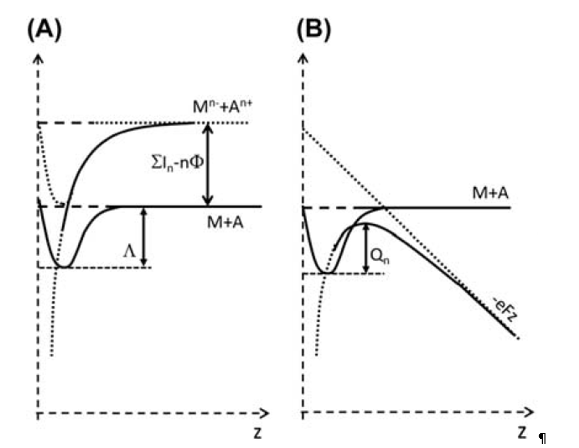
\includegraphics[width=\textwidth]{mullerenergy} \\ а)
	\end{minipage}
	%\hfill
	\begin{minipage}[b][][b]{0.49\textwidth}\centering
		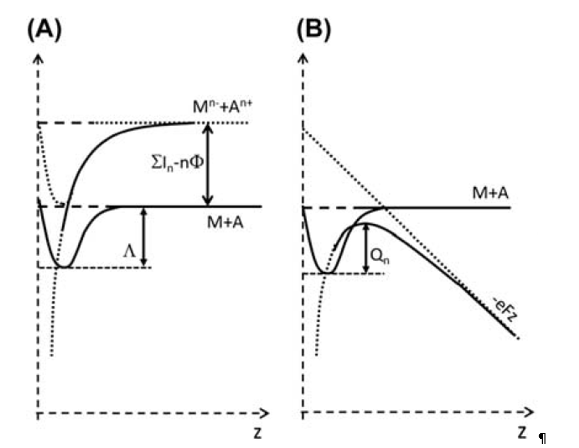
\includegraphics[width=\textwidth]{mullerenergy} \\ б)
	\end{minipage}
	\caption{Диаграмма потенциальной энергии атома без приложенного электрического поля (а), с приложенным электрическим полем (б)}
	\label{fig:mulener}
\end{figure}

Приложив внешнее электрическое поле к образцу, можно снизить потенциальный барьер, необходимый для испарения атома. Высота барьера Q(F) может быть описана следующей формулой \cite{Muller56}:

\begin{equation}
	\label{eq:equation2}
	Q(F) = Q_0 - \sqrt{\frac{n^3 e^3}{4\pi\epsilon_0}F}
\end{equation}

где $\epsilon_0$ - диэлектрическая проницаемость ьв вакууме, F - напряженность поля. Слагаемыми второго порядка, отвечающими поляризации атомов поверхности, как правило, пренебрегают. Поскольку основной задачей АЗТ является контролируемое по-атомное испарение, то необходимо контролировать скорость испарения атомов. Вероятность испарения может считаться термически активированным процессом, соответственно она может быть описана законом Аррениуса:

\begin{equation}
	\label{eq:equation3}
	P_{evap} \propto \exp(-\frac{Q(F)}{k_B T})
\end{equation}

где Q(F) - высота энергетического барьера \cref{eq:equation2}, $k_B$ - постоянная Больцмана, T - температура образца в Кельвинах. Скорость испарения определяется как:

\begin{equation}
	\label{eq:equation4}
	\Phi_{evap} = \nu_0\exp(-\frac{Q(F)}{k_B T})
\end{equation}

где $\nu_0$ - характерная частота колебаний атомов в направлении по нормали к поверхности образца. Данная зависимость подтверждена экспериментально \cite{Kellogg81,Kellogg84}, на Рисунке \cref{fig:evapspeed} представлены экспериментальные зависимости скорости испарения от приложенного электрического поля (в относительных величинах). Также наблюдались отклонения от данной зависимости \cite{Gomer84,Wada84}, которые характерны для температур менее 40 К и для ионов малой массы.

\begin{figure}[ht]
	\centerfloat{
		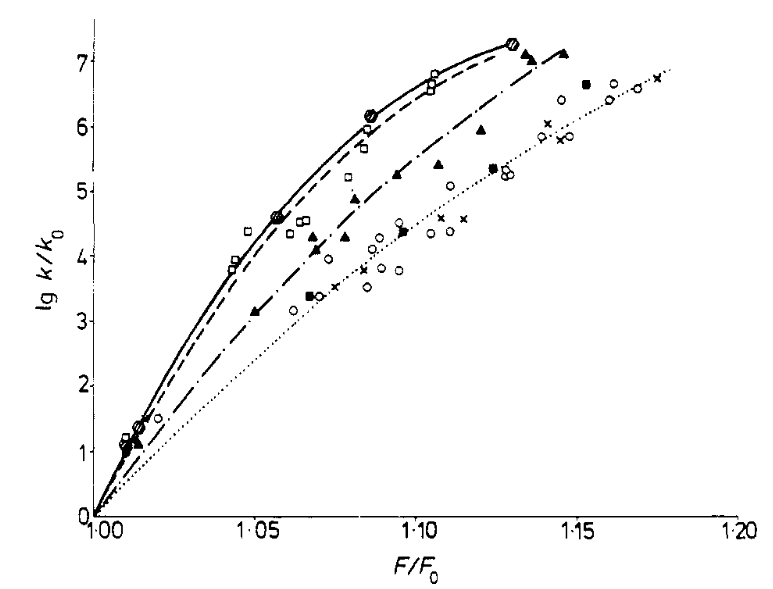
\includegraphics[scale=0.8]{evapspeed}
	}
	\caption{Зависимость скорости испарения от приложенного электрического поля для различных металлов в относительных единицах\cite{Tsong78}}
	\label{fig:evapspeed}
\end{figure} 

Значение поля, при котором величина энергетического барьера снижается до нуля, как правило, называется полем испарения $F_{evap}$. Учитывая \cref{eq:equation1} и \cref{eq:equation2}, это поле может быть вычислено для различных зарядовых состояний с помощью следующей формулы: 

\begin{equation}
	\label{eq:equation5}
	\Phi_{evap} = \frac{4\pi\epsilon_0}{n^3 e^3}(\Lambda + \sum_{1}^{n} I_n - n\phi_e)^2
\end{equation}

Результаты расчетов поля испарения для различных зарядностей ионов, на основе этого выражения, могут значительно различаться. Например, поле испарения для вольфрама принимает значения 102, 57, 52 и 62 В/нм для зарядностей +1, +2, +3 и +4, соответственно. Значения поля испарения для большинства элементов для наиболее распространенных зарядностей можно найти в справочной литературе. В работе Брандона \cite{Brandon65} было сделано предположение о том, что поле испарения определяется наименьшим из значений полей испарения для разных зарядностей иона. Данное предположение нашло хорошее подтверждение в проведенных экспериментах \cite{Tsong782}. Для большинства металлов поле испарения лежит в диапазон от 10 до 60 В/нм.
Поскольку на полевое испарение оказывает влияние температура и приложенное поле, то существует теоретически бесконечное число сочетаний значений поля и температуры, отвечающие одной и той же скорости испарения. В первом приближении высоту энергетического барьера рассматривают как величину, линейно меняющуюся весте с линейным изменением поля:
 
\begin{equation}
	\label{eq:equation6}
	Q(F) = Q_0(1 - \sqrt{1 - \sqrt{\frac{F}{F_{evap}}}}) \approx Q_0 (1 - \frac{F}{F_{evap}})
\end{equation}

Используя данное упрощенное выражение вместе с формулой \cref{eq:equation4} можно получить зависимость электрического поля необходимого для поддержания определенной скорости испарения в зависимости от температуры:

\begin{equation}
	\label{eq:equation7}
	\frac{F}{F_{evap}} \approx 1 + \ln{\frac{\Phi_{evap}}{\nu_0}\frac{k_B T}{Q_0}}
\end{equation}

Это простое выражение хорошо согласуется с экспериментальными наблюдениями различных авторов \cite{Kellogg84,Kellogg81,Wada84,Kellogg80,Vurpillot06}. Оно проиллюстрировано на Рисунке  \cref{fig:field_temp}, где поле, необходимое для испарения образца из чистого вольфрама регистрировалось как функция температуры. Соответствующее фактическое значение поля для заданной температуры обычно называют эффективным полем испарения.

\begin{figure}[tb]
	\centerfloat{
		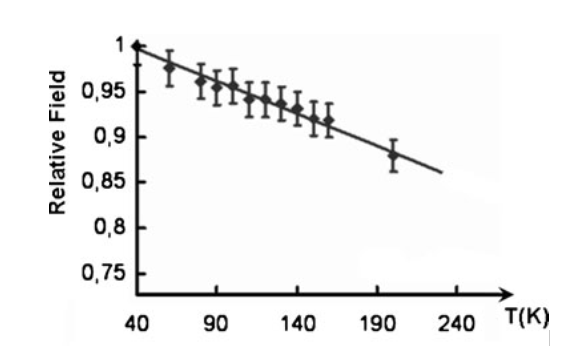
\includegraphics[scale=0.8]{field_temp}
	}
	\caption{Зависимость поля от температуры при постоянной скорости детектирования \cite{Vurpillot06}}
	\label{fig:field_temp}
\end{figure} 

\FloatBarrier


Как правило, такие кривые (как на Рисунке \cref{fig:field_temp}) используются для калибровки параметров сбора данных, то есть определения оптимальной температуры, скорости испарения и т.д. Вада, измеряя такие калибровочные кривые для чистых металлов, подчеркнул, что разные элементы будут иметь разные кривые \cite{Wada84}. При этом в сплавах будет иметь место сложная комбинация полей испарения каждого элемента в зависимости от химического состава и типов связей между элементами.

\FloatBarrier

\section{Времяпролетная масс-спектрометрия в атомно-зондовой томографии}\label{sec:ch1/sec2}

Начиная с  1967 года, когда был собран первый атомно-зондовый томограф Мюллером, Паницем и МакЛайном в Государственном университете Пенсильвании \cite{Muller68} времяпролетная масс-спектрометрия была неотъемлемой частью атомно-зондовых томографов. Простые предположения и уравнения, предложенные в то время, до сих пор регулярно используются в современных установках АЗТ для определения химической природы испаряемых ионов. Конечные результаты, такие как состав и трехмерные координаты атомов, зависят от качества обработки масс-спектра.
Качество масс-спектра зависит не только от физики полевого испарения, но и от конструкции АЗТ, условий сбора данных, характера обработки данных. В АЗТ атомы испаряются с помощью электрического поля, они ионизируются и ускоряются в электрическом поле, окружающем поверхность образца (см. общие принципы работы в разделе \cref{sec:ch1/sec4}). Некоторые из этих ионов собираются детектором, используемым для определения времени и места удара. Время полета иона – это время, необходимое для полета от поверхности образца до детектора, которое называется длиной полета L (см. Рисунок \cref{fig:time_flight}). 

\begin{figure}[htb]
	\centerfloat{
		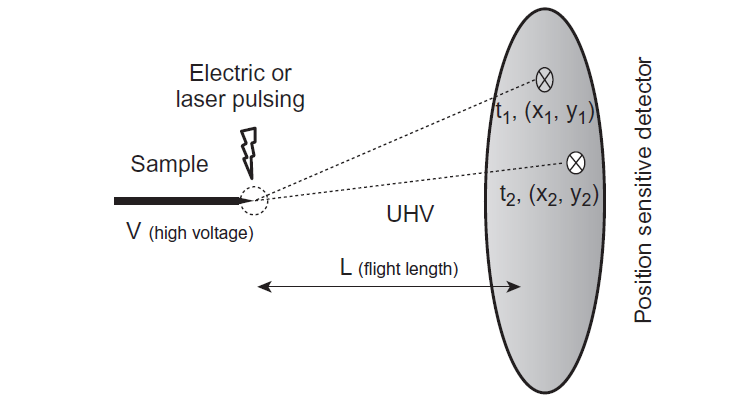
\includegraphics[scale=0.8]{time_flight}
	}
	\caption{Схема измерения времени пролета иона в АЗТ}
	\label{fig:time_flight}
\end{figure} 

Время пролета можно измерить только в том случае, если испарение инициируется напряжением или лазерным импульсом. Тогда, если предположить, что ионы не имеют начальной скорости и имеют постоянную скорость во время полета и что вся их энергия превращается в кинетическую энергию, то отношение массы к заряду M ионов записывается как:

\begin{equation}
	\label{eq:equation8}
	M = \frac{m}{n} = 2eV(\frac{t_f}{L})^2 = kV(\frac{t_f}{L})^2
\end{equation}

где m — масса иона, n — заряд, V — полное напряжение, приложенное к образцу, e — элементарный заряд электрона, L — длина полета и $t_f$ — время полета. Масса иона выражается в относительных единицах массы (а.е.м.). В современных установках АЗТ типичная длина полета составляет от 10 до 50 см, что дает характерное время полета в диапазоне около 1–5 мкс при напряжении в диапазоне 1–10 кВ.
Масс-спектр представляет собой гистограмму, высота каждого столбца гистограммы равна числу ионов задтектированных в соответствующем диапазоне масс. Как показано на Рисунке \cref{fig:mass_spectr}, на масс-спектре возможно присутствие пики, соответствующие ионам разной зарядности.

\begin{figure}[ht]
	\centerfloat{
		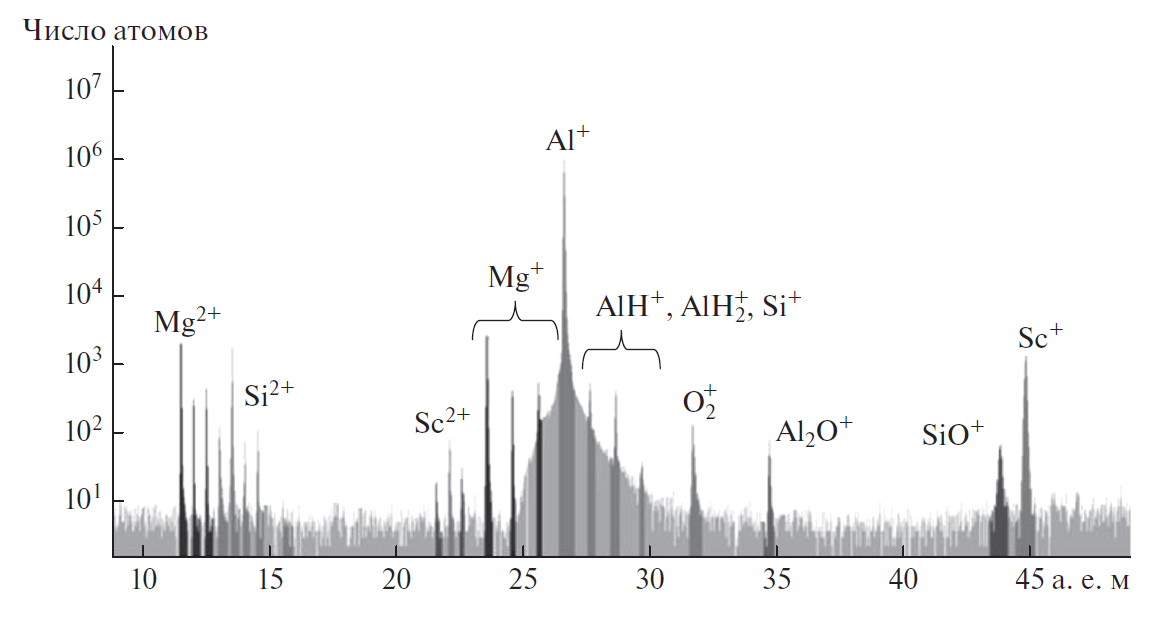
\includegraphics[width=\textwidth]{mass_spectr}
	}
	\caption{Пример масс-спектра атомно-зондовых данных, полученный в работе \cite{scbibAlumYAFI}}
	\label{fig:mass_spectr}
\end{figure} 

Идентификация пиков в масс-спектрах зависит как от предварительного знания химии анализируемого материала, так и от естественного содержания изотопов. Например, на Рисунке \cref{fig:mass_spectr} идентифицированы различные изотопы Mg$^{2+}$ (выделены в левой части спектра черным цветом). Стоит отметить, что одной из особенностей метода АЗТ является необходимость уточнения параметров восстановления масс-спектра для каждого эксперимента. Качество масс-спектра оценивают по разрешению по массе $\frac{M}{\Delta M_x}$, где $\Delta M_x$ — ширина пика масс-спектра на определенной высоте от максимальной высоты пика. Разрешение по массе обычно измеряется на уровне 50 $\%$ (полная ширина на половине высоты, FWHM), также возможны оценки на 10 $\%$ и 1 $\%$ от максимума пика. Разрешение по массе зависит от геометрических факторов (длина и траектория полета) и точности измерений (времени пролета и напряжения). Оптимизация разрешения по массе может осуществляться с помощью аппаратного обеспечения (например, рефлектронов) или применения специальных алгоритмов оптимизации при обработке данных \cite{Shutov19}.

\FloatBarrier

\section{Проекционный принцип восстановления координат атомов}\label{sec:ch1/sec3}

Как уже отмечалось, атомно-зондовая томография заимствовала принцип проекционного увеличения у автоионной микроскопии. Испаренные атомы «проецируются» на экран детектора используя расходящиеся линии электрического поля от кончика образца-иглы, что обеспечивает впечатляющее увеличение на детекторе, расположенном от образца на некотором расстоянии. Область на образце порядка 100 нм легко проецируется на детектор с радиусом в 80-120 мм, что гарантирует разрешение, близкое к атомарному \cite{Cadel09}. Используемый принцип вносит требования к условиям испарения. Для того, чтобы «зафиксировать» атомы около их равновесных положений необходимо охлаждать изучаемый образец до криогенных температур. На практике используется диапазон от 15 до 80 К. Также желание детектировать, по возможности, каждый атом требует поддержания сверхвысокого вакуума не менее $10^{-9}$ Торр.

Для того чтобы иметь возможность восстанавливать положение атома в образце необходимо измерять его координаты прилета на детектор. На сегодняшний момент наиболее подходящими являются детекторы на основе линий задержки, также использующие микроканальные пластины для увеличения сигнала от прилетевшего иона \cite{DaCosta05,Jagutzki05}. Одним из важнейших параметров МКП является коэффициент открытой поверхности, который характеризует процент площади отверстий каналов к общей площади пластины. В настоящий момент у японского производителя МКП «Hamamatsu Photonics» \cite{Hamamatsu} наилучшим коэффициентом является 90 $\%$. Этот параметр напрямую влияет на полноту и качество получаемой информации об образце.

Базовый метод заключается в восстановлении X, Y и Z координат атомов в образце по получаемым значениям $X_d$ и $Y_d$ – координатам атомов зарегистрированных на детекторе и N – номеру события детектирования атома. Первым этапом рассматриваемого алгоритма является восстановление латеральных координат атомов в образце, то есть в плоскости детектора (X, Y). Этого можно достичь путем проецирования координат, полученных с детектора на область внутри иглы по формуле \cref{eq:equation9}:

\begin{equation}
	\label{eq:equation9}
	X = \frac{X_d}{\eta}; Y = \frac{Y_d}{\eta}
\end{equation} 

где $X_d$ и $Y_d$ - координаты события на детекторе, а $\eta$ рассчитывается по формуле:

\begin{equation}
	\label{eq:equation10}
	\eta = \frac{L}{\xi r_i}
\end{equation}

\begin{equation}
	\label{eq:equation11}
	r_i = \frac{U}{k_f E}
\end{equation}

где $\xi$ - изображающий параметр, $r_i$ - радиус поверхности, с которой был испарен атом. После проведения этих вычислений необходимо получить координату Z. Изначально предполагается, что процесс испарения происходит плавно, атом за атомом, слой за слоем. Таким образом, зная о приблизительном числе атомов, находящихся в одном слое, можно восстановить глубину, с которой испарился атом. Наиболее простой и широко распространенный метод расчета был предложен Басом \cite{Bas95}. Он предлагает это делать в несколько этапов следующим образом. Сначала рассчитать элементарный сдвиг по $z_i$ по формуле \cref{eq:equation12}, а затем провести суммирование по i, для получения полного смещения i-ого атома по Z координате.

\begin{equation}
	\label{eq:equation12}
	z_i = \frac{\Omega_i}{(V_i)^2} \left(\frac{(\delta k F)^2}{\zeta d_x d_y \xi^2}\right)
\end{equation}

где  $\Omega_i$ – объем приходящийся на i-й ион, F – напряженность поля необходимая для испарения, $V_i$  - потенциал в момент испарения, $\zeta$ – эффективность детектора, $\xi$ – изображающий параметр, $d_x d_y$ – координаты частицы на детекторе.

\FloatBarrier

\section{Общие принципы работы атомно-зондового томографа. Современные установки АЗТ}\label{sec:ch1/sec4}

Исходя из широкого спектра задач по исследованию материалов существует несколько различных подходов к реализации атомно-зондовых томографов. Далее будут рассмотрены некоторые установки атомно-зондовой томографии в хронологическом порядке, отражающие передовые разработки того времени. Этот анализ позволит составить общую картину развития подобных приборов для определения наиболее оптимального вектора развития. В 1993 году во Франции был разработан один из первых приборов атомно-зондовой томографии (POSAP), который позволял получать действительно большой объем атомно-зондовых данных – информации о химической природе каждого элемента исследуемого материала в совокупности с данными о их распределении  \cite{Deconihout93}. Общая схема установки представлена на Рисунке \cref{fig:POSAP}. В данной установке использовался единственный на тот момент реально применяемый способ испарения – испарение с помощью высоковольтных импульсов. Была реализована прямо-пролетная геометрия – образец находился прямо напротив детектора.

\begin{figure}[htb]
	\centerfloat{
		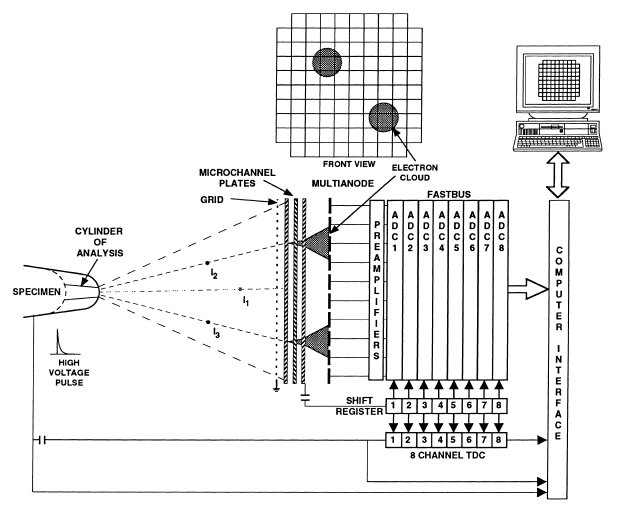
\includegraphics[width=\textwidth]{POSAP}
	}
	\caption{Схема установки POSAP \cite{Deconihout93} Specimen – образец, Microchannel plates – микроканальные пластины, Grid - сетка, Multianode - мультианод, ADC – АЦП(аналого-цифровой преобразователь), High Voltage pulse – импульс высокого напряжения, Channel TDC - канал счета времени, Computer interface – интерфейс подключения к компьютеру}
	\label{fig:POSAP}
\end{figure}

Позиционно-чувствительная детектирующая система состояла из следующих элементов: сетка нулевого потенциала, сборка из МКП, система из 10 анодов и CCD камеры. По сравнению с современными детектирующими системами, данная система отличалась низким быстродействием из-за использования CCD камеры, а также низкой способностью разделять мультисобытия, из-за малого быстродействия. Импульсное напряжение  подавалось напрямую на образец вместе с постоянной его составляющей. На данной установке было получено разрешение по массе на полувысоте ~ 300. Скорость сбора данных составляла примерно 2 иона/секунду. Площадь поперечного сечения исследуемого объема данных составляла примерно 5 × 5  нм.

Одной из первых широко распространенных и успешно используемых установок был так называемый ECOTAP – томографический атомный зонд с компенсацией энергий и оптической системой детектирования (Energy compensated optical tomographic atom probe). Его представила научному сообществу в 1998 году группа под руководством Cerezo в Оксфорде \cite{Cerezo98}. В данной установке используется импульсный высоковольтный способ испарения. Основным преимуществом этого прибора являлась реализация системы компенсации разбросов энергий ионов (рефлектрона). Как было сказано ранее, одним из основных факторов, влияющих на разрешение по массе при импульсном полевом испарении, является разброс энергий ионов, возникающий из-за статистического разброса момента испарения ионов. Соответственно, для решения этой проблемы группа Cerezo установила систему компенсации энергий типа «рефлектрон» , известную в методе времяпролетной масс-спектрометрии. Импульсная добавка напряжения для осуществления контролируемого испарения подавалась на образец с помощью контр-электрода. Контр-электрод – кольцо, расположенное напротив образца на расстоянии примерно 4 мм.

\begin{figure}[htb]
	\centerfloat{
		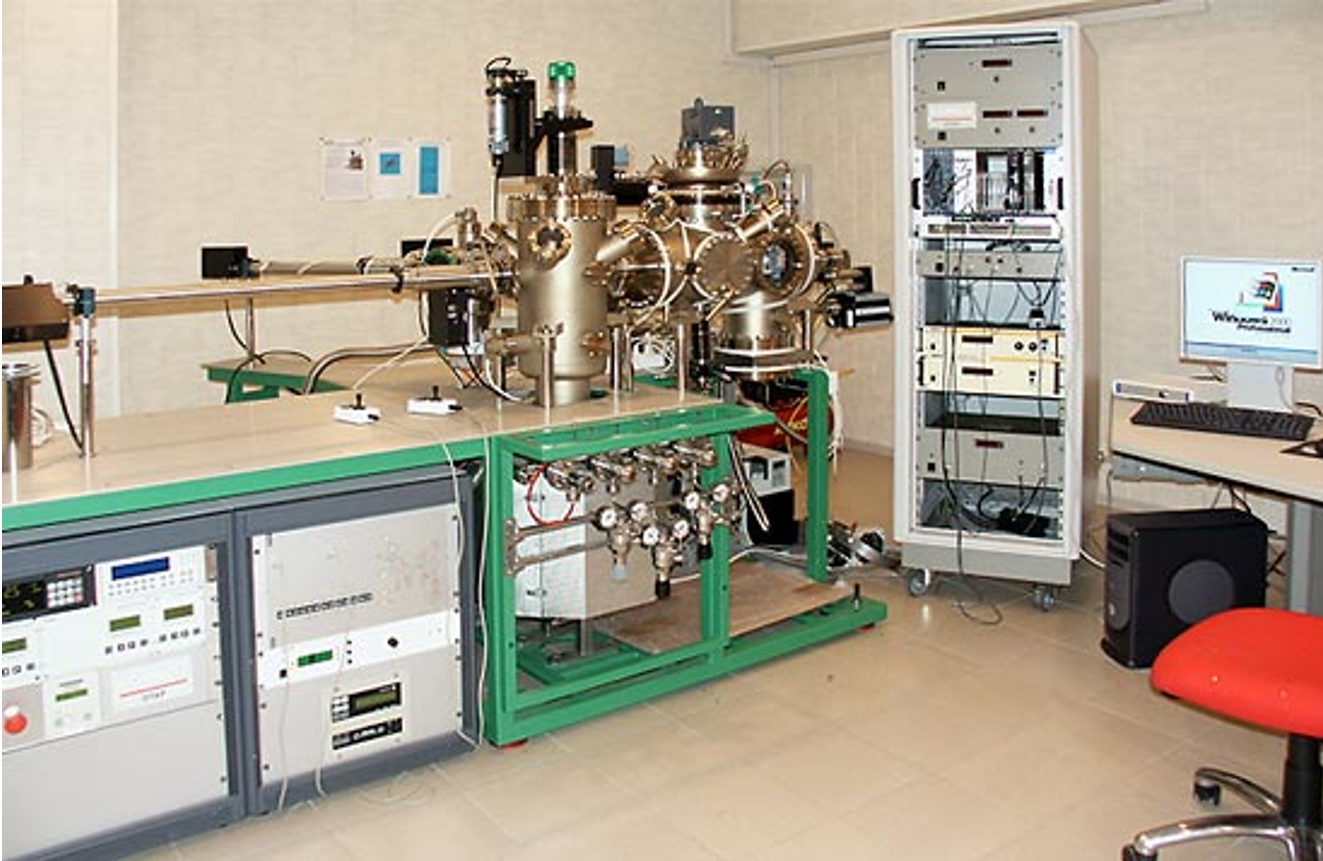
\includegraphics[width=\textwidth]{ECOTAP}
	}
	\caption{Внешний вид установки атомно-зондовой томографии CAMECA ECOTAP}
	\label{fig:ECOTAP}
\end{figure}
Данная установка позволяла получать данные следующего качества:
\begin{itemize}[beginpenalty=10000] % https://tex.stackexchange.com/a/476052/104425
	\item разрешение по массе на 50 \% высоты  $\sim$ 500;
	\item разрешение по массе на 10 \% высоты $\sim$ 250;
	\item угол сбора данных 4-12 град;
	\item сечение объема данных 20 × 20 нм.  
\end{itemize}

	
Помимо реализации рефлектрона, данная установка имела стандартные для того времени технические характеристики:
\begin{itemize}[beginpenalty=10000] % https://tex.stackexchange.com/a/476052/104425
	\item температура образцов 40-80 К;
	\item вакуум < 1 × 10$^{-9}$ Торр; 
	\item частота испаряющих импульсов 2 кГц;
	\item позиционно-чувствительный детектор c ССD камерой;
	\item напряжение на образце 20 кВ; 
	\item газо-инжекционная система;
	\item камеры хранения и загрузки образцов.
\end{itemize}


Установка типа ECOTAP производилась промышленно компанией CAMECA. Один из таких приборов был поставлен в ИТЭФ (Россия) в 2002 г. (Рисунок \cref{fig:ECOTAP}), где эксплуатируется по настоящее время \cite{Suvorov06}.

В 2000-2010 годах появилась возможность использовать компактные лазерные системы испарения, обладающие необходимой стабильностью характеристик в течении длительного времени работы. С этого момента стало возможным развивать метод лазерного  испарения в атомно-зондовых томографах. Например, в 2007 году группа под руководством Шмитца в Германии \cite{Stender07} представила установку атомно-зондовой томографии с 2-мя типами испарения (лазерное и высоковольтное импульсное) и с 3-мя различными относительными расположениями образца и детектора (для варьирования длины пролета, угла сбора данных, возможности использовать рефлектрон). На Рисунке \cref{fig:Schmitz} представлена схема расположения детекторов и вакуумных объемов данной установки. 

\begin{figure}[htb]
	\centerfloat{
		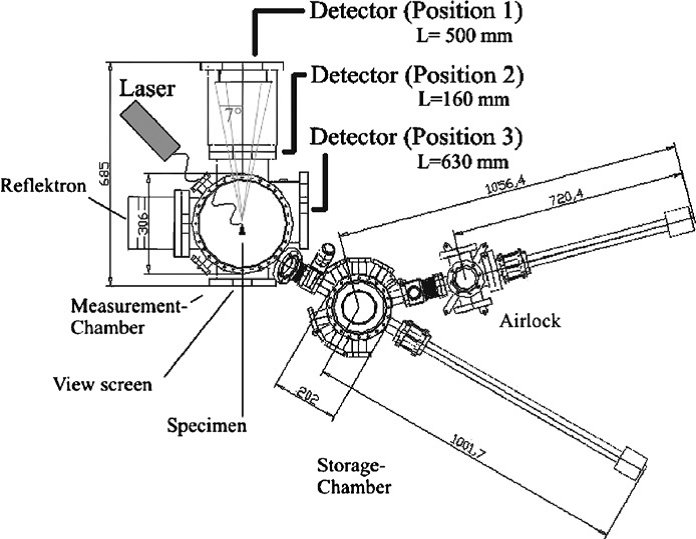
\includegraphics[width=\textwidth]{Schmitz}
	}
	\caption{Схема вакуумных объемов и положения детектирующих систем, вид сверху установки \cite{Stender07}.  Laser - лазер, Specimen - образец, Storage chamber – камера хранения образцов, View screen – смотровое окно, Airlock – камера загрузки, Measurement chamber – анализационный объем,Reflektron - рефлектрон, Detector – детектор. Все размеры на схеме указаны в мм}
	\label{fig:Schmitz}
\end{figure}

Установка, собранная научной группой Шмитца, позволяет использовать как лазерное, так и импульсно-полевое испарение. Лазерный луч находится под острым углом к оси образца. При этом в случае лазерного испарения используется прямопролетная геометрия (положение детектора №1 и №2 на Рисунке \cref{fig:Schmitz}), два различных расстояния от детектора до образца позволяют менять угол сбора данных и длину пролета, что определяет объем собираемых данных и величину разрешения по массе. В случае полевого испарения образец вместе с криосистемой поворачивается в строну рефлектрона, который используется для компенсации энергий ионов при импульсно-полевом испарении. Также, помимо основного вакуумного объема с образцом и детекторами, в состав установки входят загрузочная камера и камера хранения образцов с соответствующими штоками для перемещения образцов. Для поддержания вакуума 1-2 × 10$^{-10}$ мбар используются турбомолекулярные насосы со скоростями откачки 500/250/70 л/сек. Как уже выше было указанно, в данной установке имеется возможность поворачивать образец на 360 град вокруг вертикальной оси и ± 45 град относительно горизонтальной оси. Охлаждение образца обеспечивается с помощью двух ступенчатой криосистемы Rigon с минимальной температурой 25 К. В ходе проведения исследований различных образцов на данной установке было показано, что она имеет следующие характеристики:
\begin{itemize}[beginpenalty=10000] % https://tex.stackexchange.com/a/476052/104425
	\item угол сбора данных до 39 град;
	\item разрешение по массе 50 \% высоты $\sim$ 300;
	\item сечение объема данных 50 × 50 нм$^{2}$;
	\item среднее количество собранных данных $\sim$ 5млн.
\end{itemize}	

В 2002-2003 годах в Америке была представлена первая установка с так называемым локальным электродом LEAP\cref{fig:leap3000}.  Соответственно, наличие локального электрода обуславливало преимущество по качеству данных над большинством остальных установок и определяло дальнейшее интенсивное развитие именно данного семейства установок \cite{Kelly00}. Позднее, в 2006 г. в LEAP появилась возможность устанавливать и лазерную испаряющую систему. В таком случае постоянное напряжение по-прежнему подавалось на локальный электрод, что обеспечивало высокое разрешение по массе и более «мягкие» условия испарения.

Помимо системы испарения, данные установки отличаются наличием улучшенной версией позиционно-чувствительного детектора на основе линий задержки. Вопрос детектирования как можно большего процента испарённых ионов, а также мультисобытий, является одним из ключевых, так как он влияет на чувствительность прибора и на точность определения концентраций. С целью улучшения точности детектирования в установках LEAP используется дополнительный анод уже к двум имеющимся на детекторе. Таким образом, данная детектирующая система позволяет различать наибольшее число мультисобытий из всех существующих ныне позиционно-чувствительных детекторов, применяющихся в АЗТ.
Вакуумная система на LEAP построена по наиболее распространенной схеме. Но если камера проведения анализа или камера хранения по функционалу практически не отличаются от аналогичных установок, то камера загрузки может быть оборудована специальной системой плазменной очистки локальных электродов для продления срока их службы. Вакуум 2 × 10$^{-10}$ мбар в анализационном объеме обеспечивают как турбомолекулярные насосы, так и ионный насос с титановой присадкой. Все вакуумные объемы приспособлены для отжига до температуры ~ 150 °С.
Как уже упоминалось, на LEAP может быть установлены как импульсно-полевая, так и лазерная системы испарения. Также существует возможность заказать установку с 2 типами системы испарения. Соответственно, во всех случаях, когда присутствует полевая система испарения, установка дополняется системой компенсации энергий ионов.

Процент детектируемых ионов имеет значение 50 \% для варианта установки с энергокомпенсирующей системой и 80 \% для системы с прямопролетной геометрией. Порог чувствительности к детектированию элементов малых концентраций в анализируемом образце находится на уровне 3-7 ppm (частиц на миллион).
Импульсный источник напряжения может генерировать импульсы с амплитудой до 1400 В. Частота следования импульсов может составлять до 500 кГц. Постоянное напряжение на образце может варьироваться до 15 кВ. Лазерная испаряющая система может работать на частотах вплоть до 2 МГц.
Длительность лазерного импульса - менее 1 пс. Диаметр пучка лазера на образце принимает значения от 3 до 10 мкм, в зависимости от настройки фокусировки. В силу малости диаметра пучка, а также для повышения стабильности условий испарения в процессе эксперимента, программа управления установкой в ходе сбора данных периодически проводит автоматическую проверку наведения пучка.

\begin{figure}[htb]
	\centerfloat{
		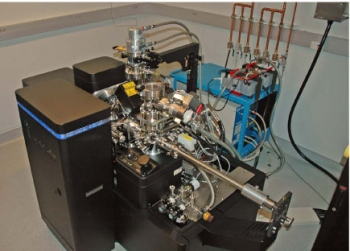
\includegraphics[scale=1]{leap3000}
	}
	\caption{Внешний вид установки атомно-зондовой томографии LEAP 3000X}
	\label{fig:leap3000}
\end{figure}

Получаемое разрешение по массе на установках сильно зависит от исследуемого материала и типа испарения. Как правило, разрешение по массе на полувысоте для лазерного испарения не опускается ниже 1000, но может достигать и значений в 1500. Для вариантов с импульсным высоковольтным  испарением разрешение по массе на полувысоте составляет примерно 400 -1000. Угол сбора данных также сильно зависит от материала и условий исследования, но максимальное заявленное сечение получаемого объема составляет 250 × 250 нм.

В настоящий момент CAMECA предлагает две ключевых конфигурации установки атомно-зондовой томографии LEAP 6000(Invisio 6000) и EIKOS. LEAP позиционируется как наиболее полный и многофункциональный инструмента для широкого круга самых передовых научных задач. Он может быть оснащен лазерным, полевым испарением, а также одновременным испарением с помощью и лазера и импульсного напряжения. Данная установка может быть дополнены криогенной съемной загрузочной камерой (ссылка на криотрансфер), которая позволяет исследовать жидкие объекты в замороженном состоянии (ссылка). Длина волны лазерной системы составляет 257,5 нм. EIKOS  позиционируется как простая и менее требовательная к квалификации персонала и к пробоподготовке установка. Одним из основных её применений производитель видит - промышленность. Ниже на Рисунках \cref{fig:EIKOS,fig:LEAP6000} представлен внешний вид EIKOS и LEAP 6000 соответственно.

\begin{figure}[htb]
	\centerfloat{
		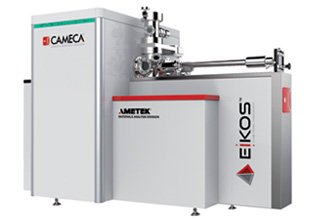
\includegraphics[scale=0.8]{EIKOS}
	}
	\caption{Внешний вид установки атомно-зондовой томографии EIKOS}
	\label{fig:EIKOS}
\end{figure}

\begin{figure}[htb]
	\centerfloat{
		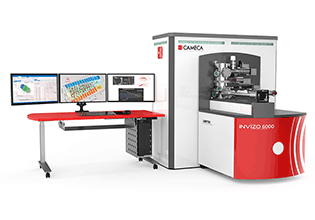
\includegraphics[scale=0.8]{LEAP6000}
	}
	\caption{Внешний вид установки атомно-зондовой томографии LEAP 6000}
	\label{fig:LEAP6000}
\end{figure}

\FloatBarrier

Среди современных установок также стоит отметить попытки создания комплексных устройств, включающих в себя комбинацию атомно-зондового томографа и другой аналитической установки или методики. В качестве второй установки может выступать СЭМ с ФИП, как в концепции группы Stender \cite{Stender22} или сканирующий туннельный микроскоп, как в концепции группы Umemura \cite{Umemura19}. Также для ряда задач, например для изучения динамики каталитических процессов, атомно-зондовые томографы могут оснащаться дополнительным оборудованием, например газовыми реакторами \cite{Lambeets20}.

\section{Влияние параметров исследования на качество данных. Калибровка атомно-зондового томографа}\label{sec:ch1/sec5}

Здесь что-то о влиянии параметров.
Сначала нужно что-то рассказать для введения в тему.
Перечень параметров, влияющих на данные.
Почему для разных установок (и для разных материалов)- разные параметры

Одним из самых важных параметров лазерной системы для применения в атомно-зондовой томографии является используемая длина волны, оказывающая значительное влияние на разрешение по массе. На Рисунке \cref{fig:Wavelength} приведены результаты модельных экспериментов - карты поглощения излучения для алюминиевого образца при различных длинах волн \cite{Houard10}.

\begin{figure}[htb]
	\centerfloat{
		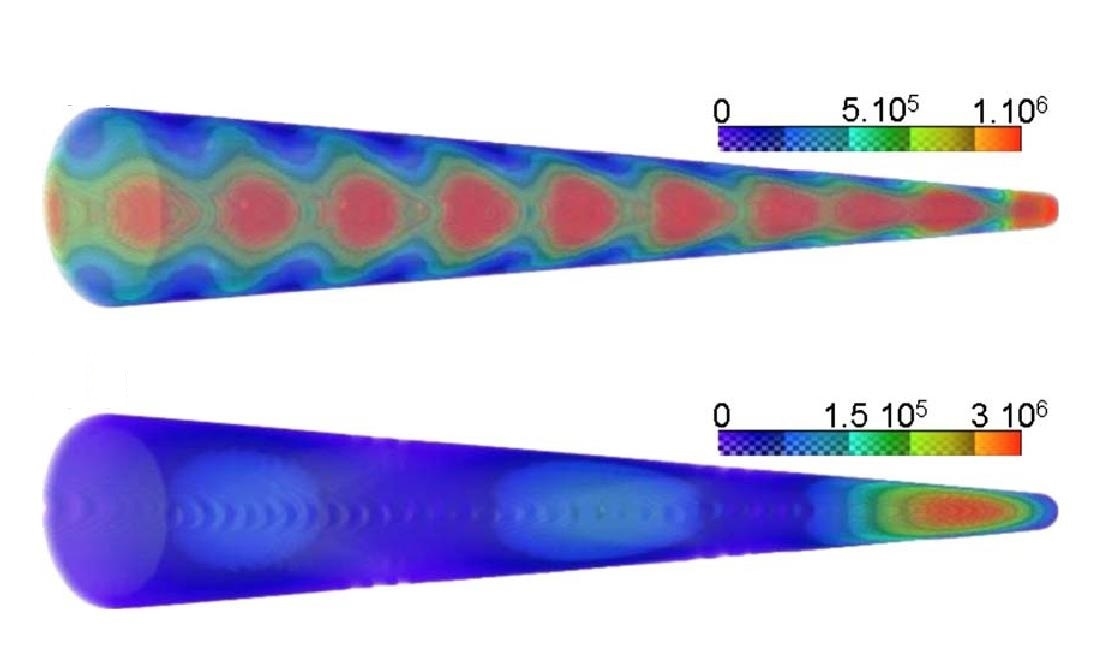
\includegraphics[width=.8\textwidth]{Wavelength}
	}
	\caption{Карты поглощения лазерного излучения образцом из Al для разных длин волн: a – распределение интенсивности излучения (Вт/см$^{2}$) при $\lambda = $ 360 нм,    б – $\lambda = $ 1200 нм \cite{Houard10}}
	\label{fig:Wavelength}
\end{figure}
Как видно, максимально нагретая область при уменьшении длины волны оказывается ближе к вершине образца, а также уменьшается ее размер, что должно положительно сказываться на разрешении по массе за счет большей скорости остывания вершины из-за возрастающего градиента температур. Этот факт подтверждается экспериментально при варьировании длины волны в эксперименте \cite{Houard10} с алюминиевым и стальным образцами (Рисунок \cref{fig:WavelengthSteelAlum})

\begin{figure}[htb]
	\centerfloat{
		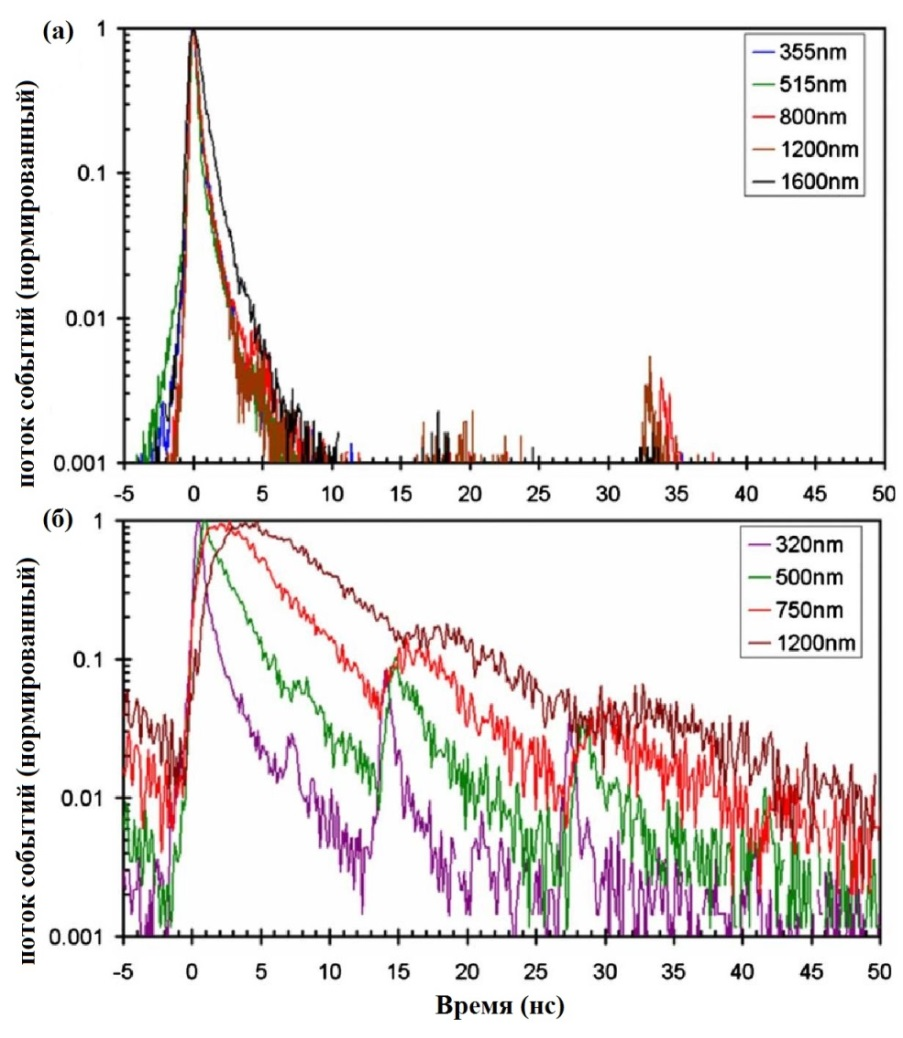
\includegraphics[width=.8\textwidth]{WavelengthSteelAlum}
	}
	\caption{Зависимость потока событий от времени после воздействия лазером для образца из алюминия (а) и стали (б) для разных длин волн \cite{Houard10}}
	\label{fig:WavelengthSteelAlum}
\end{figure}

Энергией импульса регулируется величина передаваемой энергии образцу за импульс (энергия образца определяет пиковую температуру приповерхностного слоя образца). От этого параметра зависит вероятность испарения атома (поток событий), точность определения химического состава, пространственное разрешение. Известная из основ полевого испарения \cite{GaultBOOK} зависимость напряжения на образце, при котором происходит испарение, от температуры образца (в частности приповерхностного слоя), представлена на Рисунке \cref{fig:field_temp}.

Следовательно, чем выше нагрев приповерхностного слоя образца, тем меньшее напряжение на образце необходимо для достижения заданной скорости испарения, и наоборот. Регулируя мощность лазерного импульса, можно проводить контролируемое испарение вещества при напряжениях на образце менее порогового, кратковременно нагревая приповерхностный слой до той температуры, при которой испарение осуществляется с некоторой выбранной вероятностью. Сверху мощность лазера ограничена рядом эффектов, среди которых важными являются: поверхностная миграция, абляция, а также отклонение детектируемой концентрации элементов от реального значения. В работе \cite{Cerezo07} показано, что при избыточной мощности лазера происходит падение пространственного разрешения вследствие перегрева образца (см. Рисунок \cref{fig:ParamsEnergy}).

\begin{figure}[htb]
	\centerfloat{
		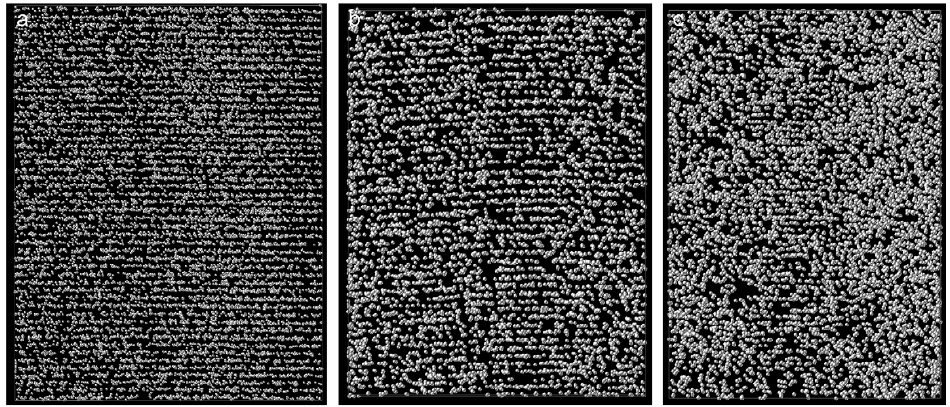
\includegraphics[width=\textwidth]{ParamsEnergy}
	}
	\caption{Срез 3D изображений образца из W, полученных при трех энергиях импульса лазера – 0.4, 1.6 и 2.0 нДж, соответственно \cite{Cerezo07}}
	\label{fig:ParamsEnergy}
\end{figure}

Исследования зависимости разрешения по массе от энергии импульса показывают, что с ростом последней, разрешение по массе увеличивается \cite{Tu15}. Это связывается с тем, что при увеличении нагрева вершины образца, градиент температуры вдоль его оси увеличивается, ускоряя процесс охлаждения, что приводит к минимизации теплового «хвоста» (Рисунок \cref{fig:ParamsPower}).

\begin{figure}[htb]
	\centerfloat{
		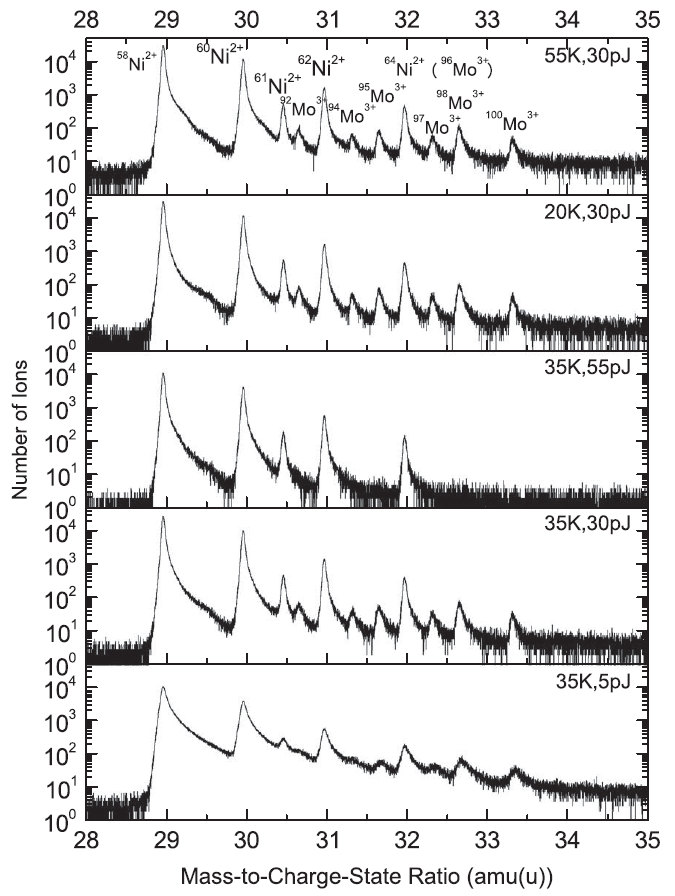
\includegraphics[width=.8\textwidth]{ParamsPower}
	}
	\caption{Сравнение масс-спектров при различной мощности лазера. Разрешение по массе возрастает с 400 до 750 на полувысоте основного пика с увеличением мощности от 5 пДж до 55пДж \cite{Tu15}}
	\label{fig:ParamsPower}
\end{figure}

Той же научной группой исследованы зависимости концентраций элементов, полученные при исследовании модельного сплава Ni-Al-Mo (Рисунок \cref{fig:ParamsComposition}) при различной энергии импульса.

\begin{figure}[htb]
	\centerfloat{
		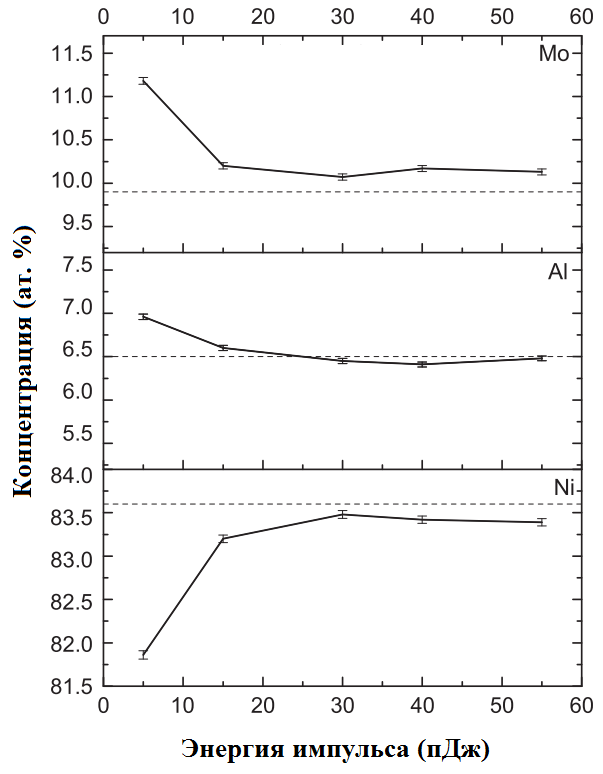
\includegraphics[width=.8\textwidth]{ParamsComposition}
	}
	\caption{Зависимость детектируемых концентраций элементов сплава Ni-Al-Mo от энергии импульса лазера при температуре образца 35 К \cite{Tu15}. Пунктирными линиями обозначены истинные концентрации элементов}
	\label{fig:ParamsComposition}
\end{figure}


Как видно, отклонение детектируемых концентраций элементов от истинных значений велико при малой энергии импульса, и уменьшается при ее возрастании. Для приведенных данных оптимальная мощность для оценки концентраций выбрана примерно в середине диапазона мощности лазерной системы, где ошибка одновременно по трем элементам сплава наименьшая. Однако утверждается, что с возрастанием мощности лазера разница в полях испарения элементов, составляющих материал, уменьшается, что благоприятно сказывается на точности определения концентрации. Но, как уже было отмечено, мощность ограничена сверху эффектами поверхностной миграции, а также нарушениями в составе испаряемых элементов (например, за счет испарения молекулярных ионов, таких как ионы $Mo^{+2}$) \cite{Tu15}. Поэтому энергия импульса, с целью улучшения разрешения по массе и точности определения концентраций, должна выбираться максимально возможной в пределах, ограниченных эффектами перегрева образца \cite{Tu15}. Также следует отметить, что, в случае исследования диэлектрических включений в металлах, для достижения точного стехиометрического состава, необходимо несколько снижать энергию импульса, по сравнению со случаем исследования металла без таких включений \cite{LarsonBOOK}.
\FloatBarrier
Еще одним важным параметром пучка для АЗТ с лазерным испарением является его поляризация. Хорошо известен эффект анизотропии поглощения, когда энергия лазера при разной поляризации по-разному поглощается образцом \cite{Houard10,GaultBOOK}. Наиболее выгодной для методики АЗТ является поляризация вдоль оси образца. В этом случае поглощенная энергия локализуется преимущественно на вершине образца, и в меньшей степени на остальной освещаемой лазерным лучом области \cite{Houard10}.

Скорость сбора данных, прежде всего, зависит от частоты импульсных воздействий на образец, активирующих процесс испарения. С одной стороны, эти импульсы должны быть максимально частыми, чтобы увеличить скорость сбора данных. Однако существует два ограничения. Первое присуще методике в целом – коридор между импульсами должен быть достаточен, чтобы измерить время пролета всех ионов. Второе ограничение, присущее АЗТ с лазерным испарением, состоит в том, что образец должен успевать охлаждаться в перерывах между импульсами. Оба этих фактора накладывают ограничение по частоте примерно до 100 кГц \cite{Cerezo07}.

Поскольку разброс ионов по времени вылета, главным образом, сопряжен со скоростью остывания вершины образца, важно рассмотреть процесс отвода тепла, обусловленный теплопроводностью. Очевидно, что отвод тепла будет расти с увеличением угла и радиуса при вершине образца. Этот эффект подтверждается экспериментально \cite{Arnoldi12}. Зависимость разрешения по массе от угла при вершине приведена на Рисунке \cref{fig:ParamsGeometry}. Зависимость разрешения по массе от радиуса при вершине приведена на Рисунке \cref{fig:ParamsGeometry}.

\begin{figure}[htb]
	\centerfloat{
		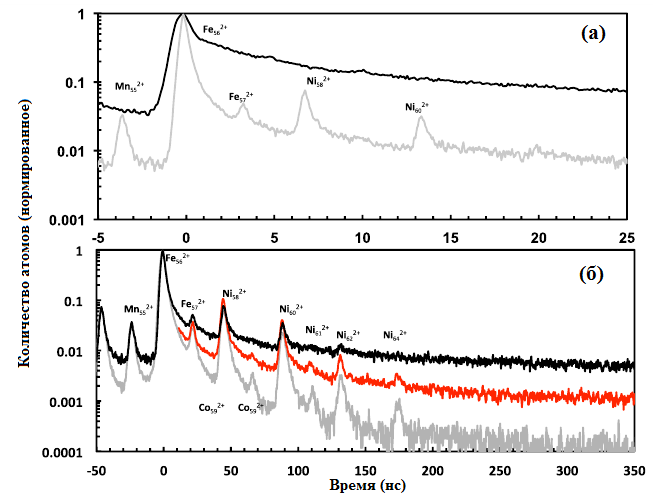
\includegraphics[width=.8\textwidth]{ParamsGeometry}
	}
	\caption{Масс спектры, полученные для стали Fe-19Cr-7Ni-3Si при разной геометрии образцов: a – при фиксированной конусности образца (5$\pm$1)\textdegree и разном радиусе при вершине (черная линия - 30$\pm$5нм, серая - 60$\pm$5нм); б – при фиксированном радиусе при вершине, но различной конусности (черная линия – (5$\pm$1)\textdegree, красная - (15$\pm$1)\textdegree, серая - (28$\pm$1)\textdegree) \cite{Arnoldi12}}
	\label{fig:ParamsGeometry}
\end{figure}

\FloatBarrier

Исследования группы \cite{Arnoldi12} также показывают, что форма образца вносит существенный вклад в качество данных. Наиболее качественные данные (речь идет об определении хим. состава) получаются при исследовании образцов с наибольшей конусностью ($\sim$28\textdegree для стали) и наибольшим начальным радиусом при вершине ($\sim$60 нм).

Базовая температура образца в атомно-зондовой томографии влияет в основном на пространственное разрешение \cite{GaultBOOK}  и точность определения концентраций. Сложность точного определения соотношений элементов исследуемого материала в данной методике обусловлена различием в полях испарения для каждого элемента. В случае высоковольтного импульсного испарения образец все время находится при определенной низкой температуре и разница в полях испарения элементов постоянна. Регулируя температуру образца, можно менять поля испарения, и, соответственно, разницу между полями испарения \cite{Wada84}.
В случае лазерного испарения базовая температура также влияет на детектируемое значение концентрации элементов. Пример зависимости измеренной концентрации модельного сплава Ni-Al-Mo приведен на Рисунке \cref{fig:ParamsTemperatureComposition}.

\begin{figure}[htb]
	\centerfloat{
		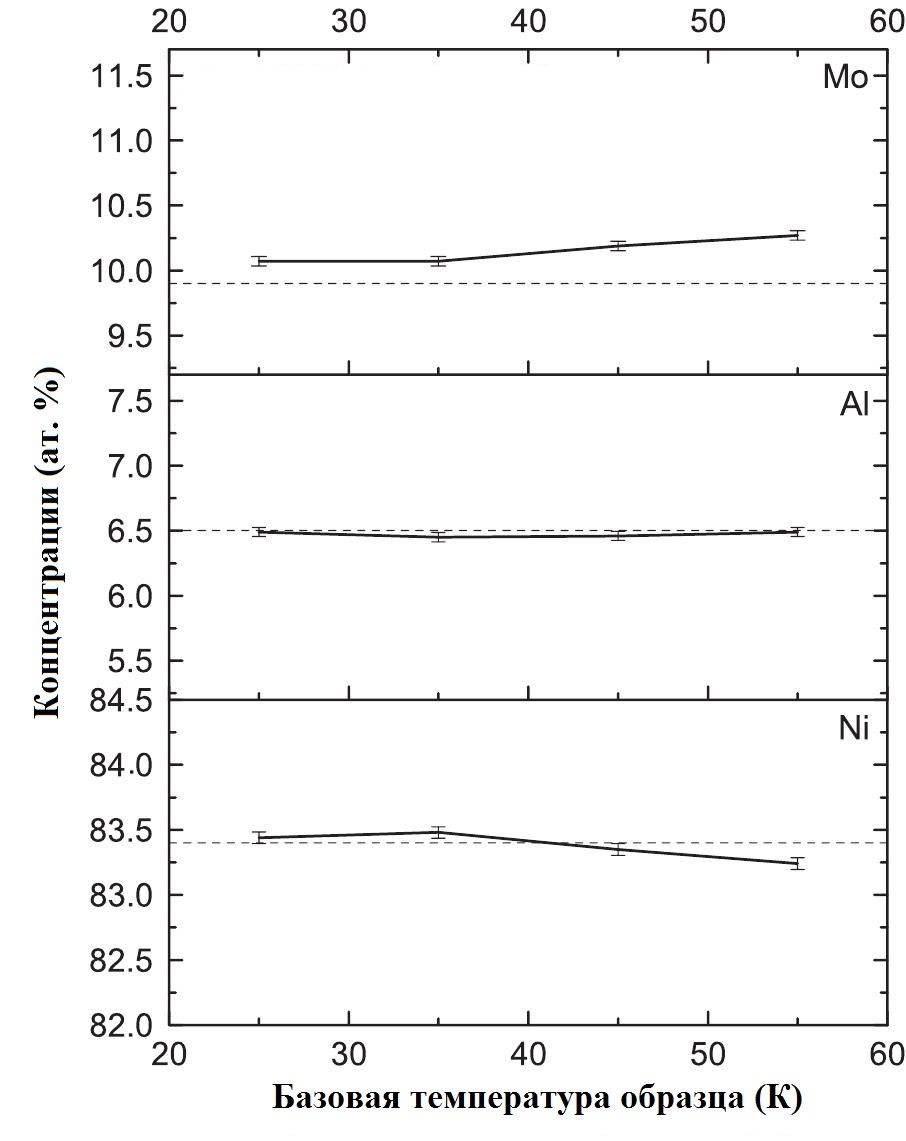
\includegraphics[width=.7\textwidth]{ParamsTemperatureComposition}
	}
	\caption{Зависимость измеренной концентраций элементов от температуры образца для модельного сплава Ni-6.5Al-9.9Mo при энергии в импульсе 30 пДж \cite{Tu15}}
	\label{fig:ParamsTemperatureComposition}
\end{figure}

\FloatBarrier

Какое-то заключение о том:

- нужно разработать АЗТ
- выбрать геометрию, узлы и т.д.
- калибровать по простому материалу
- разработать методики калибровки восстановения данных
- что параметры надо подбирать, но делать это с умом (то есть не все и не сразу)
- провести демонстрационные исследования


























           % Глава 1
\chapter{Разработка  Прототипа атомно-зондового томографа с лазерным испарением}\label{ch:ch2}

Разработки атомно-зондовой томографии в ИТЭФ (Россия) получили развитие в связи с модернизацией Центра атомно-масштабных и ядерно-физических микроскопических исследований конденсированных сред для получения разносторонней информации о наномасштабном состоянии различных материалов КАМИКС, включенного в перечень уникальных установок уникальных ядерно-физических установок, необходимых для осуществления национальным исследовательским центром «Курчатовский институт» своей деятельности (Распоряжение от 30 декабря 2009 г. №2125-р). Для расширения спектра исследований, проводящихся в ИТЭФ, в 2011 г. было принято решение о начале разработки стенда атомно-зондовой томографии нового поколения. В 2015 г. в ИТЭФ был запущен томографический атомный зонд с лазерным испарением и прямопролетной схемой конфигурации образца и детектора (см., Рис. 7, 8) \cite{scbibAPPLE}. Установка получила сокращенное название ПАЗЛ-3D – Прототип Атомного Зонда с Лазерным испарением. 

\section{Общая схема ПАЗЛ-3D}\label{sec:ch2/sec1}

Выбор общей схемы

Преимущества

Недостатки

Общая концепция

В качестве детектирующей системы выбран позиционно чувствительный DLD детектор, позволяющий существенно повысить скорость сбора данных более чем на порядок по сравнению с имеющейся в лаборатории установкой ECOTAP. Он также позволяет с высокой точностью детектировать мультисобытия (одновременное попадание нескольких частиц на детектор).

картинка схема

картинка фото


Прямопролетная геометрия позволяет избежать сложностей с настройкой дополнительных отклоняющих ионы систем (ссылка), а также позволяет применять стандартные алгоритмы восстановления данных [ссылка].  При проведении атомно-зондового исследования необходимо обеспечивать сверхвысокий вакуум в анализационном объеме. Схема расположения вакуумных объемов представлена на Рис. 9.

картинка схема





\FloatBarrier

\section{Вакуумная и криогенная системы}\label{sec:ch2/sec2}

Откачка вакуумных объемов производится с помощью двух и трех ступенчатых систем насосов фирмы Pfeiffer Vacuum для загрузочного и анализационного объемов. Первой ступенью для обоих объемов выступает сухой спиральный форвакуумный насос. Он обеспечивает разряжение порядка 10-3 Торр. Далее установлены турбомолекулярные насосы, один на загрузочной камере и два на анализационном объеме. Давление в камерах измеряется с помощью ионизационных вакуумметров с горячим катодом. В анализационном объеме давление составляет 5.0 × 10-10 Торр, в загрузочном объеме – 4.0 × 10-9 Торр.

Криогенная система, тип, причины выбора, особенности, возможности

\FloatBarrier

\section{Система испарения}\label{sec:ch2/sec3}

Для испарения атомов (ионов) на образец подается постоянное напряжение с помощью источника высоковольтного напряжения марки FuG Electronik GmbH (до 13 кВ). В качестве импульсного источника испарения используется лазерная система TEAT-25ST производства Авеста-Проект г. Москва. Данная система позволяет генерировать импульсы длительностью 60 или 300 фемтосекунд (в зависимости от настройки). Энергия импульса лежит в диапазоне от 0.1 до 250 мкДж. Основная длина волны составляет 1030 нанометров, из которой генерируются три гармоники для испарения образца: 515, 343 и 257 нанометров. Данные длины волн позволяют исследовать как металлы и полупроводники [Inoue K., Yano F., Nishida A., Takamizawa H., Tsunomura T., Nagai Y., Hasegawa M. // Ultramicroscopy. 2009. V. 109. P. 1479. DOI: 10.1016/j.ultramic.2009.08.002], так и некоторые диэлектрики [Gault B., Menand A., de Geuser F., Deconihout B., Danoix R. // Appl. Phys. Lett. 2006. V. 88. P. 14101. DOI: 10.1063/1.2186394]. Частота работы лазера составляет 50 кГц. Лазерное излучение фокусируется с помощью системы линз на кончик образца-иглы. Луч лазера заводится в камеру исследования с помощью системы зеркал и шаговых двигателей, обеспечивающей точность позиционирования менее 2 мкм. Введение лазерного луча в вакуумный объем проводится через специальное кварцевое окно с коэффициентом пропускания более 99\% для любой из 3-х гармоник. Также лазерная система генерирует синхроимпульс для измерения времени пролета частиц, который далее подается на вход модуля АЦП в детектирующей системе.
 Картинка
 
 Описание картинки

\FloatBarrier

\section{Детектирующая система}\label{sec:ch2/sec4}

В качестве базового варианта был выбран детектор производства RoentDek GmbH DLD120 с эффективным диаметром 120 мм, так как данная немецкая фирма производит наиболее современные позиционно-чувствительные детекторы на основе линий задержки для детектирования ионов. Детектирующая система состоит из сборки микроканальных пластин (МКП) и системы анодов, усилителя сигнала с детектора и аналого-цифрового преобразователя (АЦП) для оцифровки и передачи данных на компьютер. Оцифровка проводится с частотой дискретизации 5 ГГц для сигнала с МКП и с частотой 1 ГГц для сигналов с анодов. 

Принцип детектирования основан на линиях задержки и состоит в следующем. [ссылка??]. Ускоренный в поле вблизи образца ион попадает в канал МКП, порождает облако электронов, далее электроны попадают на систему анодов, наводя в проволоке анодов ЭДС. 

Картинка работы детектора

Затем сигнал усиливается в модуле усиления и передается на АЦП. 

Картинка АЦП и усилителя

Координаты прилета частиц на детекторе определяются с точностью менее 100 мкм, что позволяет обеспечить пространственное разрешение прототипа, близкое к атомарному (области образца с радиусом 50 нм ставится в соответствие область детектора с радиусом 60 мм). Эффективная площадь детектора вместе с длиной пролета ионов 183 мм позволяют достичь угла сбора данных 32, что сопоставимо с аналогичными установками [ссылка].

\FloatBarrier

\section{Программное обеспечение для управления сбором атомно-зондовых данных}\label{sec:ch2/sec5}

Основное требование к данному программному комплексу 
В рамках разрабатываемого лабораторного образца комплекса атомно-зондовой томографии необходим комплекс программ ЭВМ для управления, сбора.
Основные задачи данного ПО:
Сбор данных с АЦП подключенного к детектирующей системе
Управления напряжением, задаваемым высоковольтной системой на образце
Мониторинг показателей вакуума в различных узлах установки
Управление узлами установки при помощи интерактивной схемы
Мониторинг потока событий с возможностью коррекции текущего напряжения в зависимости от его величины
Мониторинг распределения событий на позиционно чувствительном детекторе
Мониторинг событий на масс-спектре для предварительного анализа химического состава исследуемого образца

Программа сбора данных и управления лабораторным образцом атомно-зондовой томографии ЛабОбр-сбор (далее ПО) является настольным приложением для персонального компьютера. Работа с приложением производится в операционной системе Windows. Управление ПО производится посредством взаимодействия с графическим пользовательским интерфейсом (GUI) после запуска приложения путем запуска файла с расширением .exe. Данная программа разработана в среде разработки Visual studio при помощи компилятора mvsc x64 2015, с использованием библиотек Qt 5.15.2, qwt, и других свободно распространяемых библиотек или библиотек, шедших в комплекте с поставляемым оборудованием. Начальное окно интерфейса ПО представлено на рисунке 4.13.

рисунок ПО

описание картинки 3д, слежение за напряжением, слежение за потоком


Задачи обработки данных:
1) загрузка
2) 3Д восстановление
3) масс-спектр
4) поиск кластеров
5) проксиграммы
6) частотные анализы
7) взаимодействие с БД

Картинки примера обработки


\FloatBarrier

Заключение к главе - собран атомно-зондовый томограф, уникальный для России, преимущества:
- концепт, схема, ПО, логика работы - всё сделано своими силами
- лазерное испарение
- собственное ПО сбора и обработки данных










           % Глава 2
\chapter{Калибровка атомно-зондового томографа ПАЗЛ-3D}\label{ch:ch3}

\section{Верификация точности восстановления координат}\label{sec:ch3/sect1}

Оценка пространственного разрешения атомно-зондового томографа обычно заключается в исследовании чистого металла с последующим определением наличия/отсутствия атомных плоскостей. В случае, если пространственное разрешение установки равно или меньше чем расстояние между атомными плоскостями, разрешение установки считается равным или меньше чем расстояние атомными плоскостями, отвечающими тому или иному кристаллографическому направлению. Для верификации точности восстановления 3D координат был выбран поликристаллический вольфрам \cite{scbibAPPLE}. Данный материал имеет ряд преимуществ для калибровочных процедур, таких как: отсутствие оксидного слоя, высокую температуру плавления, простоту изготовления образцов и кубическую объемно-центрированную решетку с параметром решетки 0.316 нм. Для подтверждения характеристик использовалось не менее 3 успешных исследований материала. Условия проведения исследования: температура образцов не более 22 К, частота работы лазера 25 кГц, мощность лазерного излучения не более 20 мВт, длина волны лазерного излучения 515 нм, скорость сбора данных от 60 до 250 событий/секунду. Пример полученного масс-спектра показан на рисунке \cref{fig:W_massspectr}. На масс-спектре отчетливо различимы пики всех стабильных изотопов вольфрама. Наблюдаемая зарядность ионов составила 3+. 

\begin{figure}[htb]
	\centerfloat{
		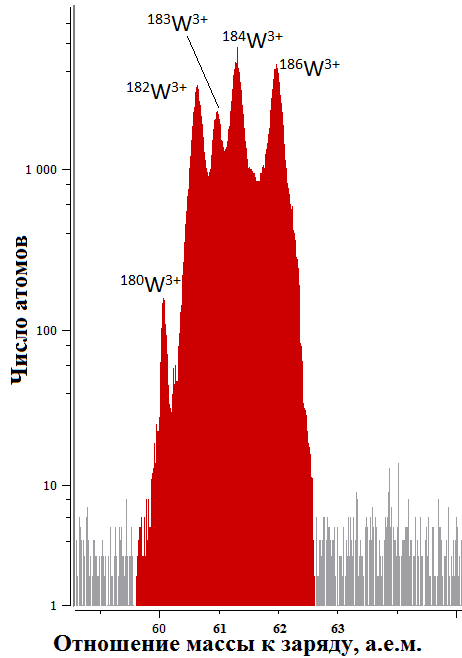
\includegraphics[width=.5\textwidth]{W_massspectr}
	}
	\caption{Масс-спектр образца из вольфрама}
	\label{fig:W_massspectr}
\end{figure}

Для оценки расстояния между атомными плоскостями были взяты отдельный части 3D объема в местах выхода кристаллографических направлений. Области выхода кристаллографических направлений определялись по двумерной гистограмме распределения событий на детектирующей системе, собранных за некоторый промежуток времени (Рисунок \cref{fig:W_3D}).

\begin{figure}[htb]
	\centerfloat{
		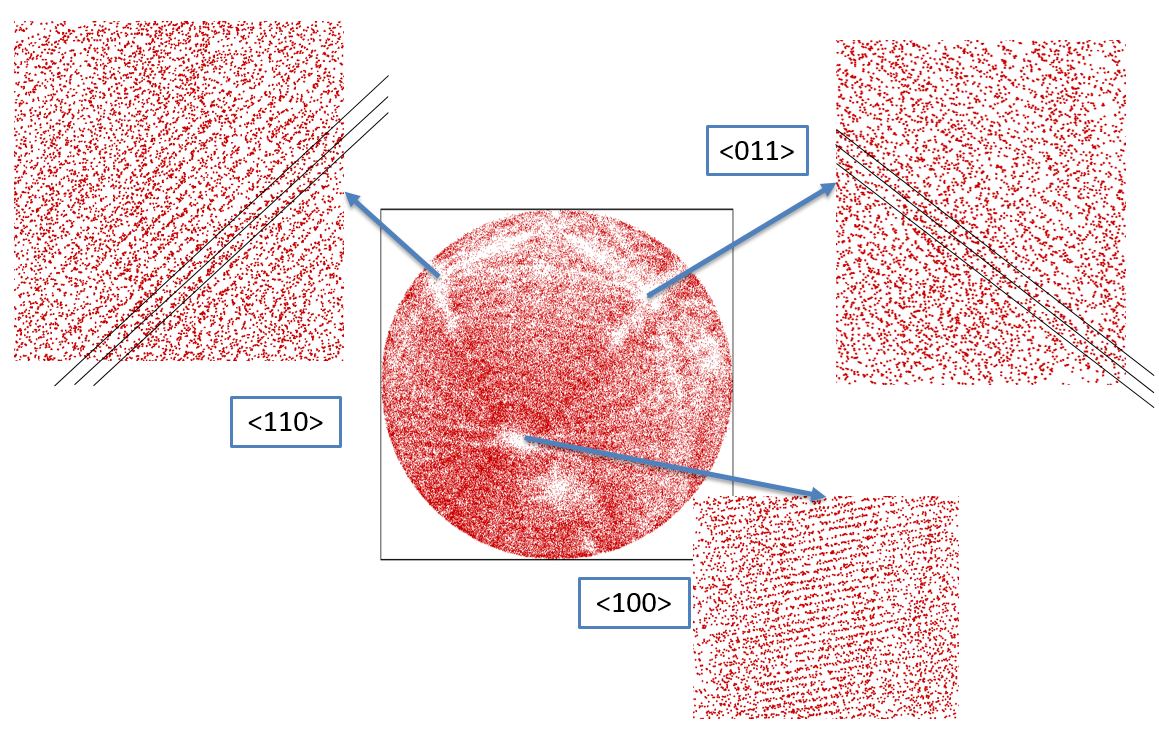
\includegraphics[width=\textwidth]{W_3D}
	}
	\caption{2D гистограмма распределения задетектированных событий}
	\label{fig:W_3D}
\end{figure}

Для каждого набора атомных плоскостей было определено среднее межплоскостное расстояние. Для выхода (100) измеренное расстояние составило 1.58 $\pm$ 0.03 \r{А}, что совпадает с табличным значение для вольфрама 1.58 \r{A} в переделах погрешности. Поскольку выход (100) ориентирован вдоль оси образца, то способность установки наблюдать атомные плоскости позволяет оценить разрешающую способность прибора вдоль оси образца (Z) в не более чем 1-2 \r{A}. Для выходов (011) также измерено межплоскостное расстояние: 1.9 $\pm$ 0.3 \r{A}, что также согласуется с табличным значением в 2.23 \r{A}. Наборы плоскостей (011) и (110) расположены под углом к оси образца, это позволяет оценить латеральное разрешение установки: 2-4 \r{A}. Полученные оценки разрешающей способности ПАЗЛ-3D не хуже аналогов и характерны для большинства атомно-зондовых томографов. 

\FloatBarrier

\section{Определение оптимальной метрики качества испарения}\label{sec:ch3/sect3}

В ходе сбора данных с одного образца ряд факторов могут приводить к изменению условий испарения материала. Например, меняется форма кончика образца(так как он постепенно испаряется), может происходить медленный "дрейф" мощности лазера или фокусировка лазерного излучения выходит из оптимального положения. Данные изменения приводят к различным артефактам испарения, которые будут влиять на результат анализа данных. Следовательно, для проведения качественных исследований необходимо разработать методику поддержания постоянных и воспроизводимых условий испарения в рамках исследования одного образца. В разделе \cref{sec:ch1/sec5} описаны основные используемые метрики для сравнения АЗТ данных. Поскольку ПАЗЛ-3D это новая разработанная установка, то для рядя исследований необходимо разработать методик сравнения результатов исследований с точки зрения возможности сравнения и воспроизводимости.

Для данной работы выбран материал Al-3.5Cu-0.2Mn-0.1S~wt\%. Это однородный материал на масштабах нескольких сотен нанометров. Также стоит отметить, что это 4-компонентный сплав, что дает возможность проследить динамику изменения концентраций нескольких элементов друг относительно друга при различных условиях испарения. Исследования проводились при постоянной температура образца 50 К. Остальные параметры менялись в ходе сбора данных. В начале работы были выбраны несколько различных метрик-кандидатов для оценки пригодности контролю условий испарения. Ниже приведен список возможных метрик:

\begin{itemize}
	\item Концентрации элементов
	\item Мощность лазерного излучения	
	\item Доля однократных событий (или общая доля мультисобытий)
	\item Доля мультисобытий одного из элементов
	\item Соотношение зарядностей основного элемента
	\item Доля шум до пика основного элемента (10-11 а.е.м.)
	\item Доля шум после пика основного элемента (40-41 а.е.м.)			
\end{itemize}

К метрикам предъявлялось несколько требований. Первое и основное - корректность получаемых концентраций элементов. Второе, не менее важное требование, это возможность вычислять значение выбранной метрики "налету" в процессе сбора данных. Также требовалась минимальная повторяемость результатов, хотя бы в рамках одного исследования. Для оценки повторяемости значений метрик данные собирались в определенном порядке. основным варьируемым параметром являлась мощность лазерного излучения. Соответственно, в ходе исследований мощность сначала поэтапно уменьшали, потом увеличивали, затем опять уменьшали. Это позволило оценить возможность воспроизводит условия испарения на протяжении всего сбора данных.  В приложении \cref{app:B} в таблицах приведены все параметры проведения исследовании и результаты расчета значений выбранных метрик. В процессе сбора данных стало понятно, что измерять напрямую концентрации элементов в процессе сбора данных не представляется возможным ввиду ресурсо-затратности методов восстановления и оптимизации масс-спектра.
Далее в работе показаны основные зависимости, которые были обнаружены или наличие которых было подтверждено(ранее они описывались для других атомно-зондовых томографов).

Наиболее очевидно и ожидаемой являлась зависимость концентрации от мощности лазерного излучения. График зависимости приведен на рисунке \cref{fig:params_Conc_Power} а). На графике точки соединены в порядке сбора данных, то есть показан наглядно, что концентрация элемента практически прямо пропорциональна мощности лазерного излучения(возможно наличие небольшого гистерезиса). Но в случае другого образца и другой фокусировки лазера (рисунок \cref{fig:params_Conc_Power} б)) уже наблюдается нелинейная зависимость. Скорее всего есть область оптимума точности сбора данных между слишком малой и слишком большой мощностями лазерного излучения. Данное предположение коррелирует с наблюдаемыми зависимостями качества данных в работе \cite{scbibOptParamsYAFI} (подробно описывалось в разделе \cref{sec:ch1/sec5}).

\begin{figure}[htb]
	\begin{minipage}[b]{0.49\textwidth}\centering
		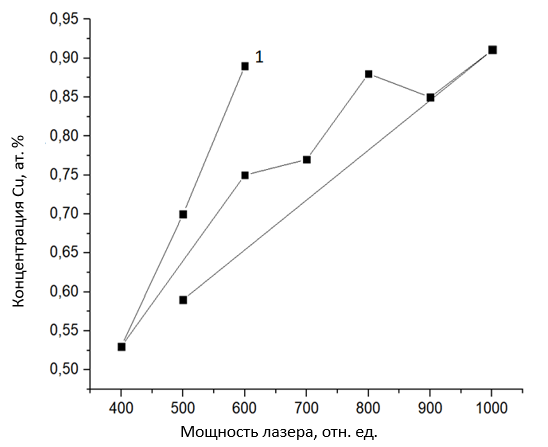
\includegraphics[width=\textwidth]{params_Conc_Power} \\ а)
	\end{minipage}
	\begin{minipage}[b]{0.49\textwidth}\centering
		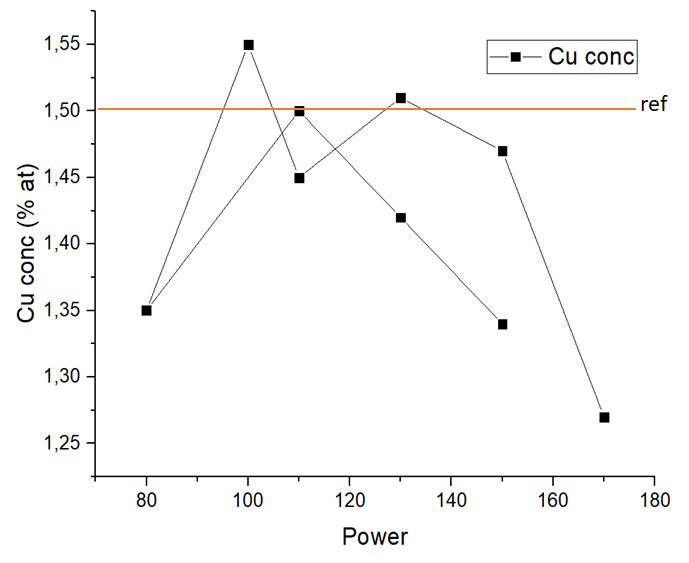
\includegraphics[width=\textwidth]{params_Conc_Power_2} \\ б)
	\end{minipage}
	\caption{Значения концентрации Cu при различной мощности лазерного излучения для двух наборов исследований. Точки соединены в порядке сбора данных. Оранжевой горизонтальной линией на отмечено табличное значение концентрации меди для исследуемого материала}
	\label{fig:params_Conc_Power}
\end{figure}

\FloatBarrier

Важно отметить, что данные для Рисунка \cref{fig:params_Conc_Power} были обработаны уже после проведения исследований. Как выше было неоднократно отмечено, что напрямую концентрации в процессе сбора данных затруднительно вычислять точно и с учетом шума/коррекций/оптимизаций.

Далее изучим другую, более перспективную метрику - соотношение зарядностей. Поскольку основным элементом в данном материале является алюминий, то была оценена зависимость концентрации меди от отношения $Al^{+}/Al^{++}$ (Рисунок \cref{fig:params_Conc_CSR}).

\begin{figure}[htb]
	\begin{minipage}[b]{0.49\textwidth}\centering
		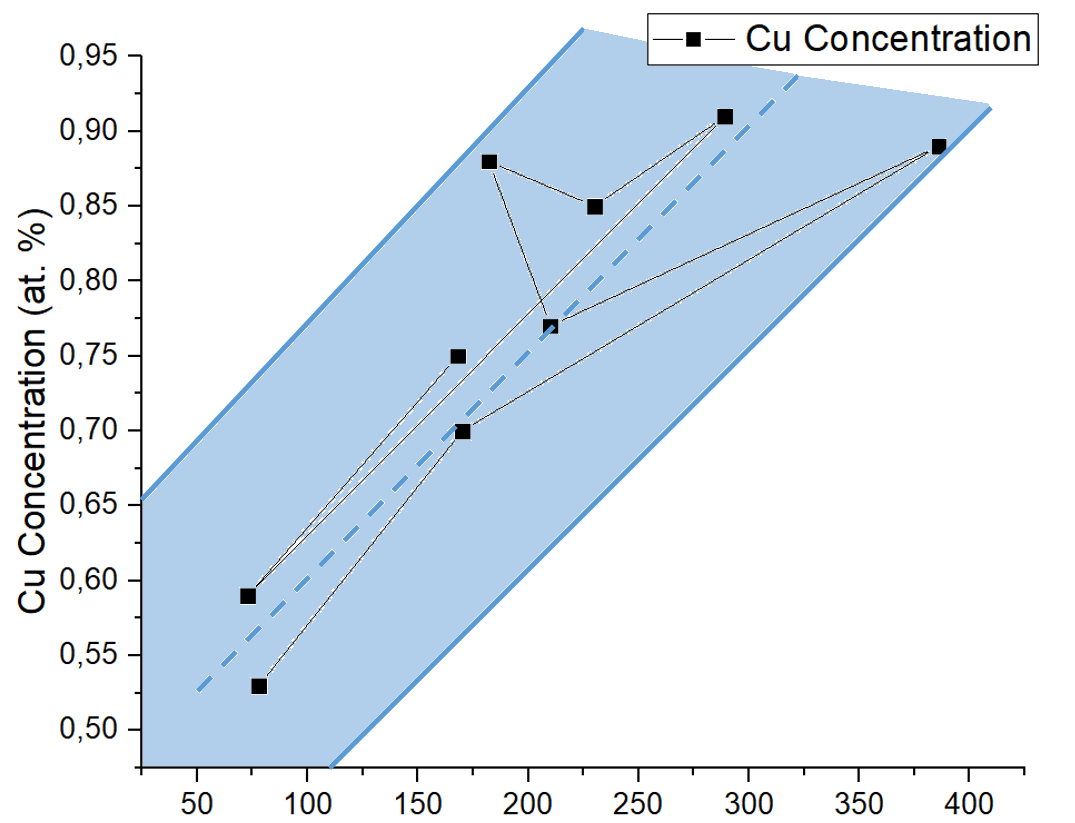
\includegraphics[width=\textwidth]{CSR_1} \\ а)
	\end{minipage}
	\begin{minipage}[b]{0.49\textwidth}\centering
		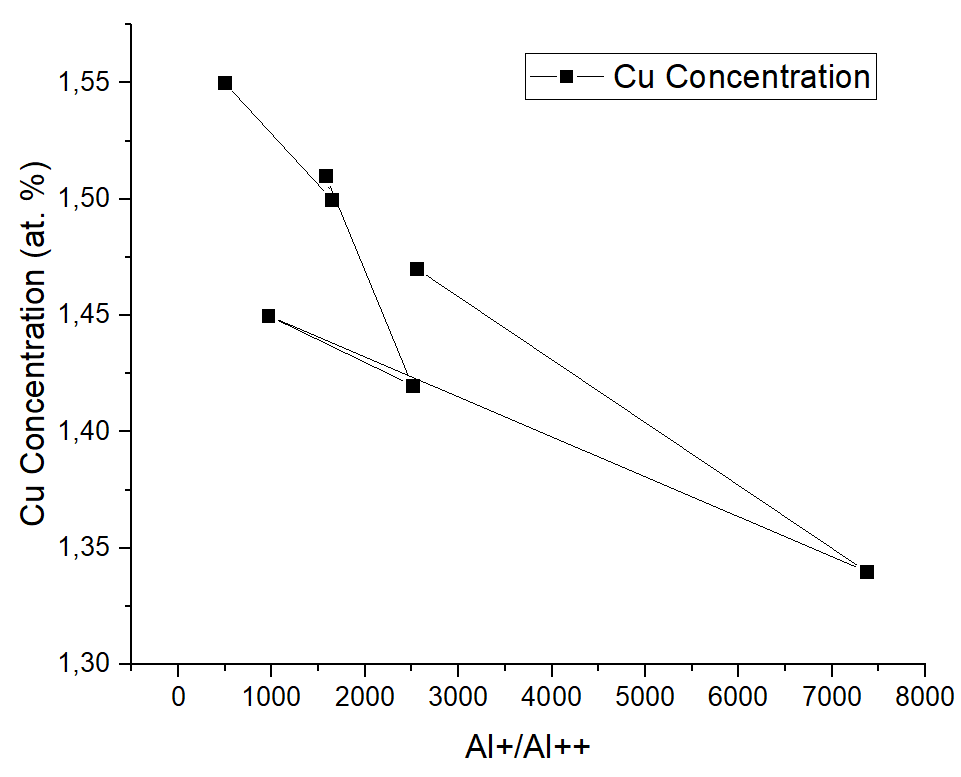
\includegraphics[width=\textwidth]{CSR_2} \\ б)
	\end{minipage}
	\caption{Значения концентрации Cu при различном соотношении зарядностей алюминия для двух наборов исследований. Точки соединены в порядке сбора данных.}
	\label{fig:params_Conc_CSR}
\end{figure}

На Рисунке \cref{fig:params_Conc_CSR} наглядно видно, что для первого набора данных концентрация меди не достигает требуемого значения в 1.52 ат. \%, но при этом явно наблюдается воспроизводимость значения концентрации при похожих значениях соотношения зарядностей. Можно аппроксимировать линейной зависимостью($y = ax + b$) с параметрами a = XXX, b = YYYYY. При этом для второго набора данных наблюдается противоположный характер зависимости. Для второго набора данных можно также провести аппроксимацию линейной зависимостью с параметрами a = XXX, b = YYYYY. Стоит отметить, что во втором наборе данных 2 промежуточные точки практически с идеальной точностью соответствуют табличному значению концентрации меди в данном материале. Аналогичный характер зависимостей наблюдался в работе \cite{Mancini14}, что подтверждает корректность предложенной методики. Для второго набора данных также построены значения концентраций других элементов  в зависимости от соотношения зарядностей алюминия. На Рисунке \cref{fig:params_Sn_Mn_O}

\begin{figure*}
	\centering
	\begin{subfigure}[b]{0.475\textwidth}
		\centering
		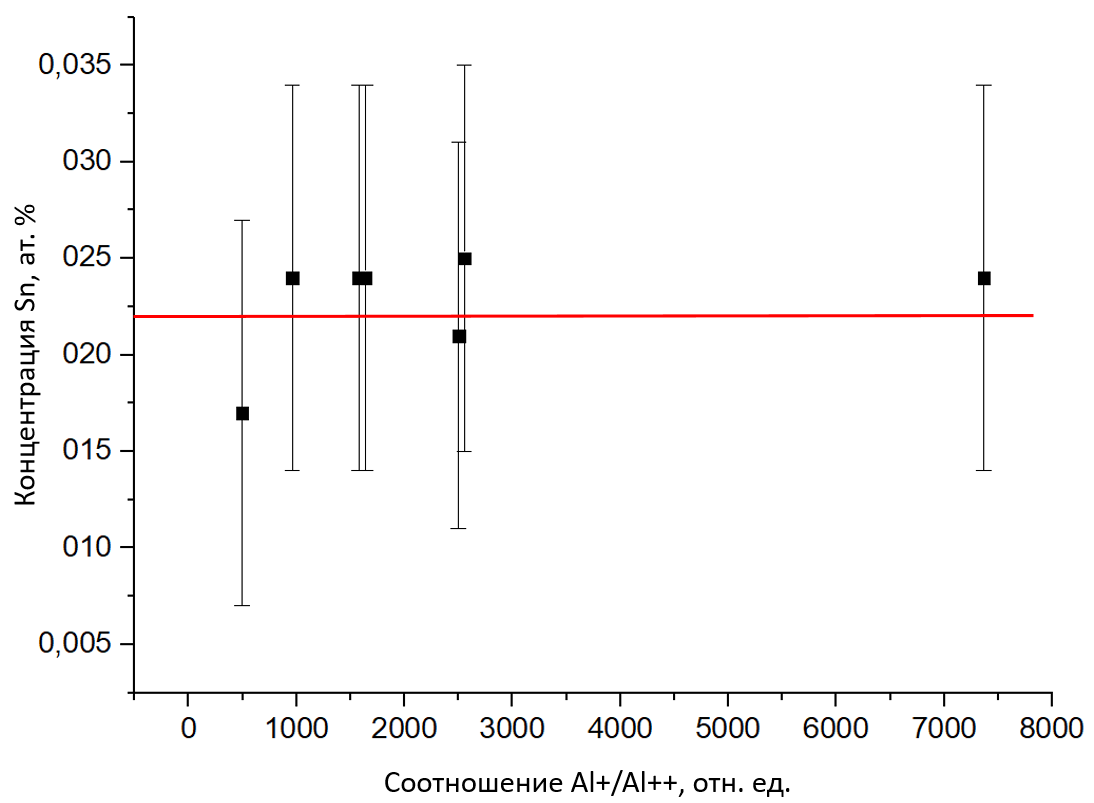
\includegraphics[width=\textwidth]{params_sn_conc}
		\caption{}    
	\end{subfigure}
	\hfill
	\begin{subfigure}[b]{0.475\textwidth}  
		\centering 
		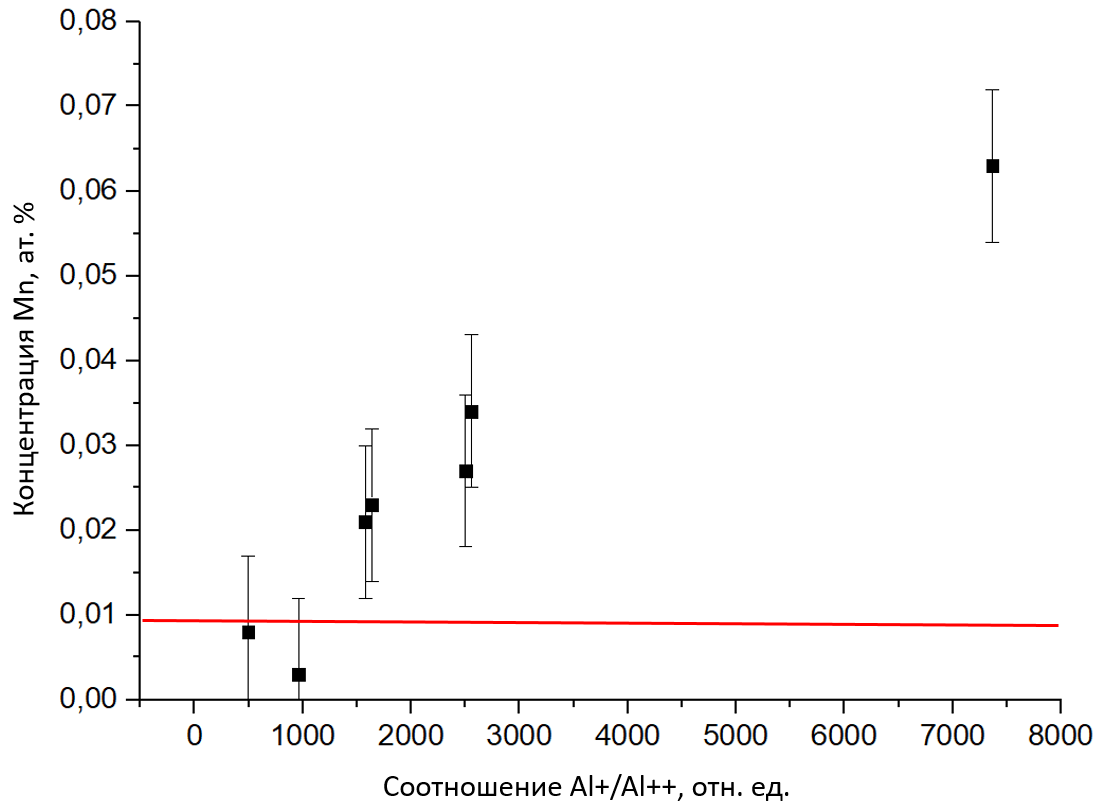
\includegraphics[width=\textwidth]{params_mn_conc}
		\caption{}    
	\end{subfigure}
	\vskip\baselineskip
	\begin{subfigure}[b]{0.475\textwidth}   
		\centering 
		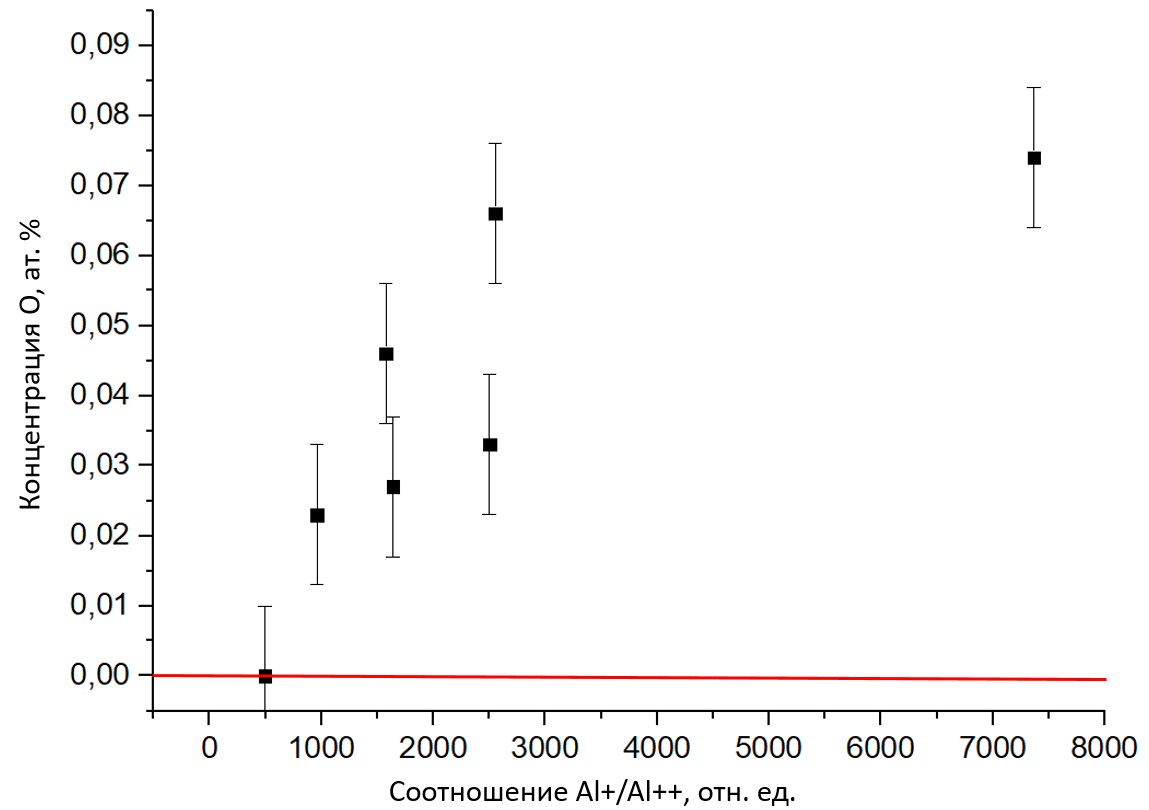
\includegraphics[width=\textwidth]{params_o_conc}
		\caption{}    
	\end{subfigure}
	\hfill
	\caption
	{Значения концентраций Sn(а), Mn(б), O(в) в зависимости от соотношения зарядностей алюминия. Красной линией указаны табличные значения концентрации для исследуемого материала   } 
	\label{fig:params_Sn_Mn_O}
\end{figure*}

Анализируя результаты, показанные на Рисунках \cref{fig:params_Conc_CSR,fig:params_Sn_Mn_O} можно заключить, что для установки ПАЗЛ-3D для алюминиевого сплава Al-3.5Cu-0.2Mn-0.1S~wt\% оптимальным диапазоном значений соотношения зарядностей является промежуток от 500 до 2000 отн. еди. В данном промежутке концентрация меди и олова наиболее близка к табличным значениям. При этом наблюдается малое количество кислорода, наличие которого является артефактом лазерного испарения. Таким образом показано, что соотношение зарядностей основного элемента может служить метрикой качества данных для алюминиевых сплавов данного типа. Показана воспроизводимость результатов исследований с использованием контроля условий испарения по соотношению зарядностей основного элемента.

При оценке зависимости качества АЗТ данных от других метрик было показано несколько второстепенных зависимостей (или показано их отсутствие):

\begin{itemize}
	\item Доля мультисобытий не является воспроизводимой метрикой для АЗТ данных.
	\item Мощность лазерного излучения пропорциональная соотношению зарядностей, но имеет плохую воспроизводимость на разных наборах данных, а следовательно точно не подходит для разных установок (Рисунок \cref{fig:params_Noise_Multi} в)).	
	\item Доля мультисобытий меди имеет понижательную тенденцию с ростом напряжения на образце
	\item Доля шум до пика основного элемента (10-11 а.е.м.) и доля шум после пика основного элемента (40-41 а.е.м.)	падают с увеличением мощности лазерного излучения и увеличиваются с ростом напряжения на образце (Рисунок \cref{fig:params_Noise_Multi} а) и б)).
	\item Доля мультисобытий меди не является воспроизводимой метрикой для АЗТ данных.	
\end{itemize}

Полученные второстепенные зависимости могут быть важны для более оптимального выбора условий испарения в дальнейших работах по развитию методик исследования алюминиевых сплавов. Также полученные корреляции могут использоваться для лучшей интерпретации данных. Все указанные метрики собраны в Таблице \cref{tab:params_expl}, в которой также приведены основные особенности и минусы их как кандидатов для основной метрики качества и воспроизводимости данных.

\begin{figure*}
	\centering
	\begin{subfigure}[b]{0.475\textwidth}
		\centering
		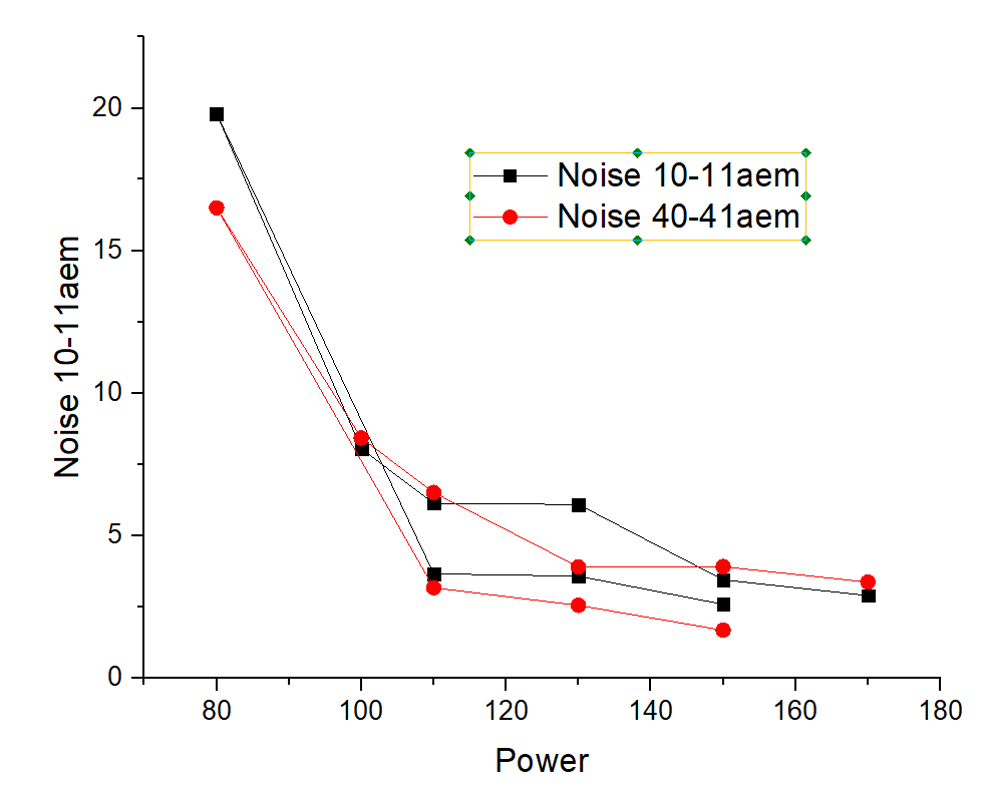
\includegraphics[width=\textwidth]{params_Noise_Power}
		\caption{}    
	\end{subfigure}
	\hfill
	\begin{subfigure}[b]{0.475\textwidth}  
		\centering 
		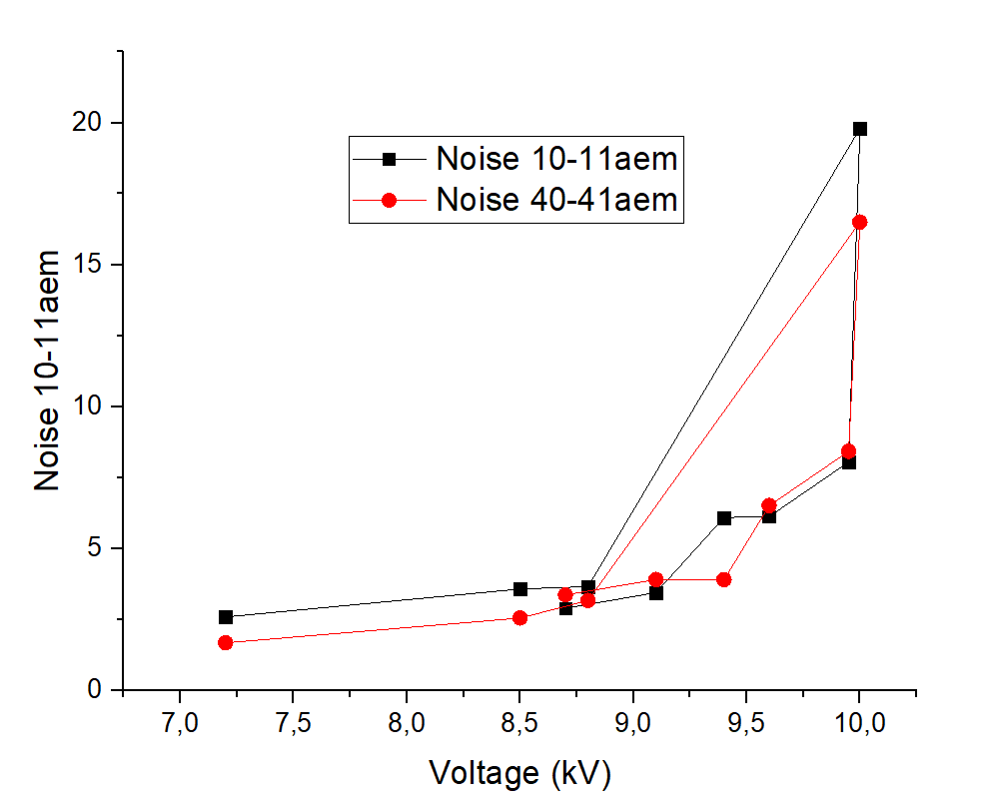
\includegraphics[width=\textwidth]{params_Noise_Voltage}
		\caption{}    
	\end{subfigure}
	\vskip\baselineskip
	\begin{subfigure}[b]{0.475\textwidth}   
		\centering 
		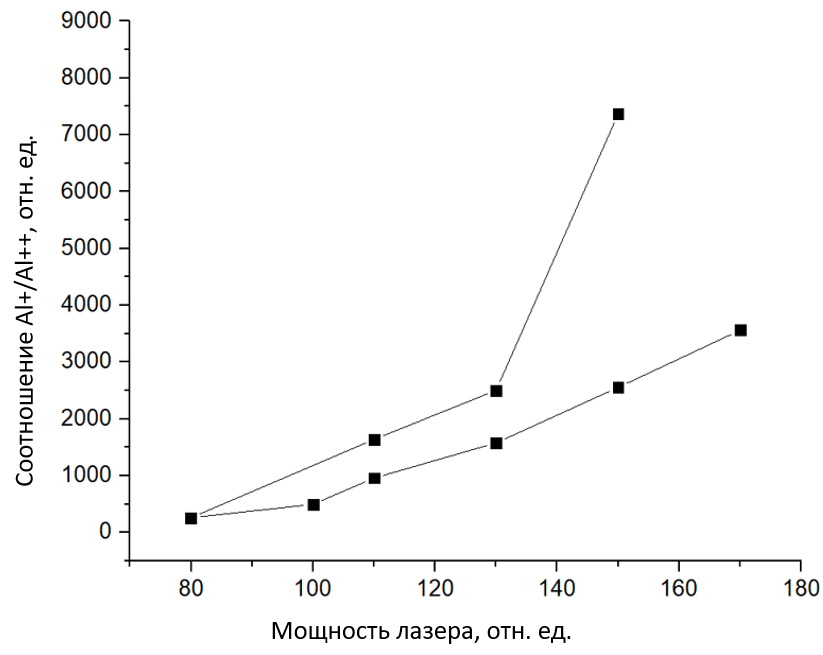
\includegraphics[width=\textwidth]{params_CSR_Power}
		\caption{}    
	\end{subfigure}
	\hfill
	\caption
	{а) - Значения шума до и после пика основного элемента от мощности лазерного излучения. б) - - Значения шума до и после пика основного элемента от напряжения на образце. в) Значения соотношения зарядностей в зависимости от мощности лазерного излучения. На всех рисунках точки соединены в порядке сбора данных} 
	\label{fig:params_Noise_Multi}
\end{figure*}

\begin{table} [htb]
	\centering
	\caption{Метрики качества атомно-зондовых данных}
	\label{tab:params_expl}
	\begin{SingleSpace}
		\begin{tabularx}{\textwidth} {| X | X | X | X |}
			\hline
			Наименование & Описание/ комментарии & Возможная интерпретация & Минусы  \\ \hline
			Однократные события & {Доля однократных событий ко всем событиям}  & {Чем больше - тем проще расшифровывать данные}  & {Нет прямой корреляции с концентрациями}              \\ \hline
			Мощность лазера & {Легко измеряется/ меняется в процессе исследования}  & {-}  & {нет повторяемости от образца к образцу}              \\ \hline
			Доля мультисобытий Cu & Возможная метрика сложности точности определения концентрации & Чем меньше - тем лучше & Нет прямой корреляции с концентрациями          \\ \hline		
			Шум на промежутке 10-11 а.е.м.      & Доля атомов с массами от 10 до 11 а.е.м. & Чем больше мощность лазера, тем меньше шума, чем выше напряжение, тем больше шума  & Нет прямой корреляции с концентрациями               \\ \hline
			Шум на промежутке 40-41 а.е.м.      & Доля атомов с массами от 40 до 41 а.е.м. & Чем больше мощность лазера, тем меньше шума, чем выше напряжение, тем больше шума  & Нет прямой корреляции с концентрациями             \\ \hline
			Концентрации  & -   &  -   & Расчет невозможен в реальном времени  \\ \hline			
			Соотношение Al$^+$/Al$^{++}$, отн. ед.    & Возможна оценка по предварительному масс-спектру, без оптимизации   & Есть значимая зависимость и повторяемость концентраций от соотношения зарядностей  & Может отличаться для разных материалов   \\ \hline
		\end{tabularx}
	\end{SingleSpace}
\end{table}

\FloatBarrier
Таким образом в результате в данном разделе показана методика выбора метрики качества и воспроизводимости АЗТ данных для алюминиевых сплавов. Выбранная метрика - соотношение зарядностей для основного химического элемента материала. Основываясь на том, что сохранение соотношения зарядностей основного химического элемента обеспечивают воспроизводимость результатов АЗТ исследований (концентрации близки к ожидаемым), можно заключить, что методика поиска оптимальных параметров испарения заключается в следующем:

\begin{itemize}
	\item собрать набор АЗТ данных при различных соотношения зарядностей основного химического элемента 
	\item рассчитать концентрации всех элементов	
	\item (дополнительно) проверить данные на отсутствие артефактов испарения (например, наличия кислорода, не входящего в состав материала)
	\item в случае неполучения целевых значений концентраций или наличия большого числа артефактов провести более широкий перебор значений соотношений зарядностей
	\item выбрать тот диапазон значений соотношений зарадностей, при котором концентрации наиболее близки к целевым значениям и при это наблюдается минимальное количество артефактов испарения
	\item в дальнейших исследованиях придерживаться выбранного диапазона
\end{itemize}

\FloatBarrier

\section{Сравнение атомно-зондовых данных для установок ПАЗЛ-3D и ECOTAP на примере сплава Al-Cu-Zr}\label{sec:ch3/sect4}

Для демонстрации методики сравнения АЗТ данных, описанной в предыдущем разделе \cref{sec:ch3/sect3} было проведены исследования на двух АЗТ установках с лазерным испарением ПАЗЛ-3D и АТЛАЗ (Модернизированная АЗТ установка АТЛАЗ была собрана на базе прибора CAMECA ECOTAP). Для исследования выбирались материалы содержащие наноразмерные кластеры. Была выбрана сталь 16Х12МВСФБР ЭП-823 \cite{Porollo04} после облучения ионами (далее ЭП-823). Данная сталь отличается высокой плотность кластеров. Вторым материалом для сравнения выбран алюминиевый сплав Al-3.3Cu-2.5Mn-0.5Zr (мас. \%) после отжига при температурах 350 \textdegree С и 450 \textdegree С \cite{Belov22,Belov21} (далее сокращенно называются как Al-Cu-Mn-Zr 350 \textdegree С и Al-Cu-Mn-Zr 450 \textdegree С соответственно). Концентрации и их погрешности был для всех исследований были рассчитаны по формулам, предложенным в работах Danoix \cite{Danoix071,Danoix072}. В качестве погрешности указано среднее отклонение от среднего значения, когда на одно обработанное состояние приходилось более одного исследования.

Критериями сравнения точности восстановления данных были выбраны следующие характеристики: разрешение по массе на полувысоте пика, разрешение по массе на 10~\% высоты пика точность определения концентраций матрицы и частиц, точность определения размеров частиц. Также использовались технические параметры для сравнения данных. Как показано в работах \cite{Tang10,Geuser07} одним из важнейших таких параметров можно считать количество и распределение мульти-событий. Для исследуемых объемов рассчитаны как общий процент мульти-событий, так и доля мульти-событий, приходящаяся на элементы, которые является кластеро-/фазо-образующими. Помимо мульти-событий, учитывались величины скорости детектирования и уровень шума.

Образцы приготовлены с помощью электрохимического утонения. Все данные на ПАЗЛ-3D и АТЛАЗ собраны при температуре образца 50~К. Мощность лазера составляла на ПАЗЛ-3D 85 $\pm$ 1 мВт и на АТЛАЗ 3 $\pm$ 0.5 мВт. Скорость сбора данных представлена ниже в таблице. Восстановление и обработка данных проводилась в ПО КВАНТМ-3D. Параметры восстановления для ПАЗЛ-3D были выбраны следующие: полевой множитель kf от 4 до 6, множитель сжатия изображения ICF от 1.2 до 1.6. Атомные карты представлены на Рисунке.  \cref{fig:APPLEvsATLAS}. Алгоритмы восстановления масс-спектра и 3D данных использовались те же, что и для вольфрама. Для определения состава включений Zr для сплава Al-Cu-Mn-Zr 350 °C, ввиду их не сферичной формы, использовались изоконцентрационные поверхности. Ниже, в Таблицах \cref{tab:paramsAPPLEvsATLAS,tab:matrixAPPLEvsATLAS,tab:clustersAPPLEvsATLAS}, представлено сравнение данных для разных установок для алюминиевого сплава.

\begin{table} [htbp]
	\centering
	\caption{Сравнение характеристик точности восстановления данных для алюминиевых сплавов Al-Cu-Mn-Zr}
	\label{tab:paramsAPPLEvsATLAS}
	\begin{SingleSpace}
		\begin{tabular} {| c | c | c | c | c |}
			\hline
			    {} & \thead{ПАЗЛ-3D, \\350 \textdegree C} & \thead{АТЛАЗ, \\350 \textdegree C} & \thead{ПАЗЛ-3D, \\450 \textdegree C} & \thead{АТЛАЗ, \\450 \textdegree C} \\ \hline
			$M/\Delta M_{50\%}$ Al$^+$ & 670  & 260  & 421  & 430               \\ \hline
			$M/\Delta M_{10\%}$ Al$^+$ & 206  & 120  & 146  & 190               \\ \hline
			Мульти-события, \%         & 0.7  & 2.9  & 0.9  & 2.9               \\ \hline
			Мульти-события Cu, \%      & 4.23 & 0.54 & 7.11 & 3.17              \\ \hline
			Мульти-события Zr, \%      & 7.31 & 0.85 & 0.18 & 0.6               \\ \hline
			Шум, 10$^{-5}$ отн. ед. & 5.4   & 1.9   & 10.7  & 1.67  \\ \hline
			Скорость сбора данных, атомов/возд.        & 0.005 & 0.006 & 0.007 & 0.007 \\ \hline
			Соотношение Al$^+$/Al$^{++}$, отн. ед.    & 640   & 310   & 630   & 450   \\ \hline
		\end{tabular}
	\end{SingleSpace}
\end{table}

Для Al-Cu-Mn-Zr 450 °С на ПАЗЛ-3D представлены средние значения характеристик данных по трем исследованным образцам. Проведено сравнение химического состава материалов как в кластерах для Al-Cu-Mn-Zr 350 °С, так и в матрице для Al-Cu-Mn-Zr 350 °С и 450 °С. Ввиду не сферичной формы включений Zr была использована методика изо-концентрационных поверхностей (поверхностей одинаковой концентрации). Для определений границ включений были построены поверхности так, чтобы перегиб профиля концентраций, построенный нормально к поверхности (проксиграмма) проходил точно на полувысоте по концентрациям \cite{Hellman07}. Параметры, используемые для построения и расчетов, были выбраны следующие: размер сетки 1-1.5 нм, делокализация 2 нм, изо-концентрация поверхности по 1.5 \% Zr. 

\begin{table} [htbp]
	\centering
	\caption{Состав кластеров [ат. \%] в алюминиевом сплаве Al-Cu-Mn-Zr после отжига при 350~°С, полученный
		на установках ПАЗЛ-3D и АТЛАЗ}
	\label{tab:matrixAPPLEvsATLAS}
	\begin{SingleSpace}
		\begin{tabular} {| c | c | c |}
			\hline
			{} & ПАЗЛ-3D & АТЛАЗ \\ \hline
			Al       & 96.9 $\pm$ 0.3  & 99.7 $\pm$ 0.4   \\ \hline
			Cu       & 0.3 $\pm$ 0.1   & 0.3 $\pm$ 0.1    \\ \hline
			Mn       & 0.04 $\pm$ 0.02 & 0.003 $\pm$ 0.002  \\ \hline
			Zr       & 2.4 $\pm$ 0.3   & 2.8 $\pm$ 0.2    \\ \hline
			Ni, C, O & Баланс & Баланс   \\ \hline			
		\end{tabular}
	\end{SingleSpace}
\end{table}

\begin{figure}[h!tb]
	\begin{minipage}[b][][b]{0.49\textwidth}\centering
		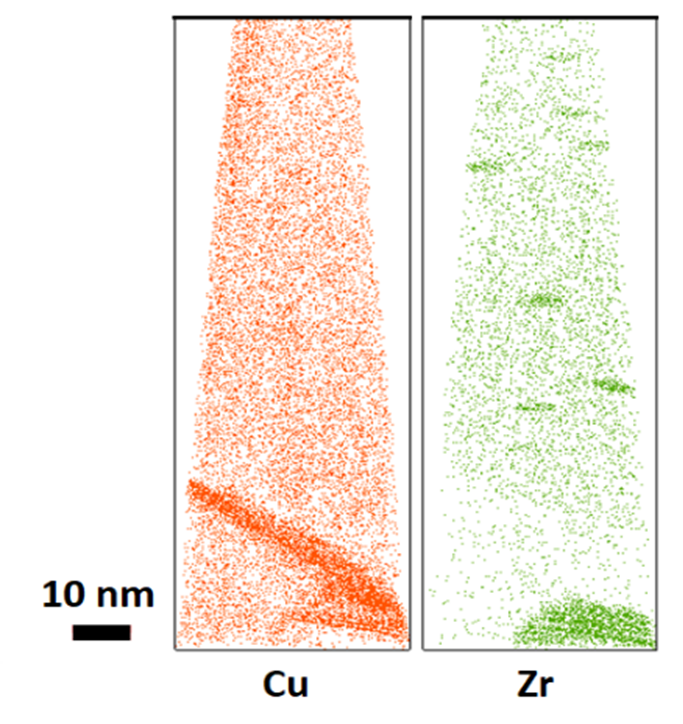
\includegraphics[scale=0.5]{APPLEvsATLAS_apple} \\ а)
	\end{minipage}
	%\hfill
	\begin{minipage}[b][][b]{0.49\textwidth}\centering
		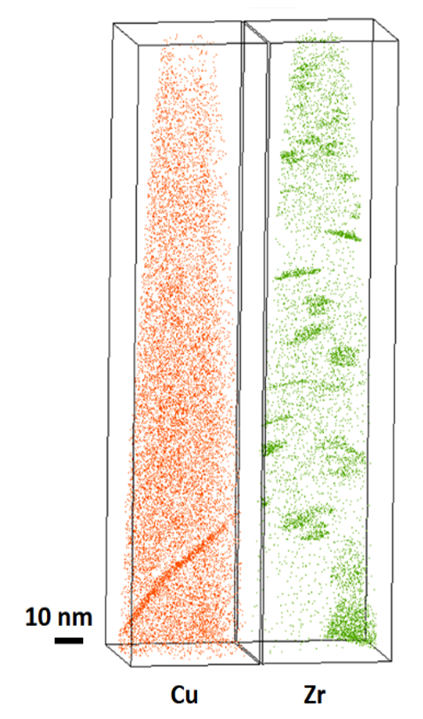
\includegraphics[scale=0.8]{APPLEvsATLAS_atlas} \\ б)
	\end{minipage}
	\caption{а) Атомные карты сплава Al-Cu-Mn-Zr 350°С ПАЗЛ-3D. б) Атомные карты сплава Al-Cu-Mn-Zr 350°С АТЛАЗ.}
	\label{fig:APPLEvsATLAS}
\end{figure} 

Данные для Al-Cu-Mn-Zr 450°С на ПАЗЛ-3D рассчитаны как среднее по трем исследованным образцам, погрешности также для данного материла рассчитаны как среднее отклонение от среднего значения. Плотность включений для данных с ПАЗЛ-3D составила (0.9 $\pm$ 0.1) x 10$^{23}$ и (1.40 $\pm$ 0.05) x 10$^{23}$ штук в м$^3$ для АТЛАЗ.

Исследование ЭП-823
Условия сбора данных были во много идентичны тем, что использовались при исследовании алюминиевых сплавов. Температура образцов составляла 50~К, мощность лазера на ПАЗЛ-3D 40 $\pm$ 1 мВт, на АТЛАЗ 2 $\pm$ 0.5 мВт. Для восстановления атомно-зондовых данных и их обработки также использовалось ПО КВАНТМ~3D и те же алгоритмы 3D восстановления. Множитель поля $k_f$ составлял 4.5, коэффициент сжатия изображения ICF от 1.2 до 1.35. Процесс обработки масс-спектра включал в себя первоначальную разметку с помощью автоматизированного инструмента разметки модуля “environment editor”, после была проведена ручная коррекция размеченных пиков. Далее был проведен пересчет пресекающихся пиков, в частности для Cr и Fe, ориентируясь на соседние пики этих элементов. Был проведен пересчет коэффициента Ni++ с целью минимизировать влияние термического хвоста Fe. Пики меди были разделены и рассмотрены на 3D модели, с целью убедиться, что оба пика соответствуют Cu. Также были проверены пики Mo на возможное пересечение с Cr+. В образце на ПАЗЛ-3D, был обнаружен пик Nb между пиками Mo, на АТЛАЗ из-за повышенного шума этот пик не виден на масс-спектре. На Рисунке \cref{fig:APPLEvsATLAS_EP} показаны атомные карты объемов.

\begin{figure}[h!tb]
	\begin{minipage}[b][][b]{0.49\textwidth}\centering
		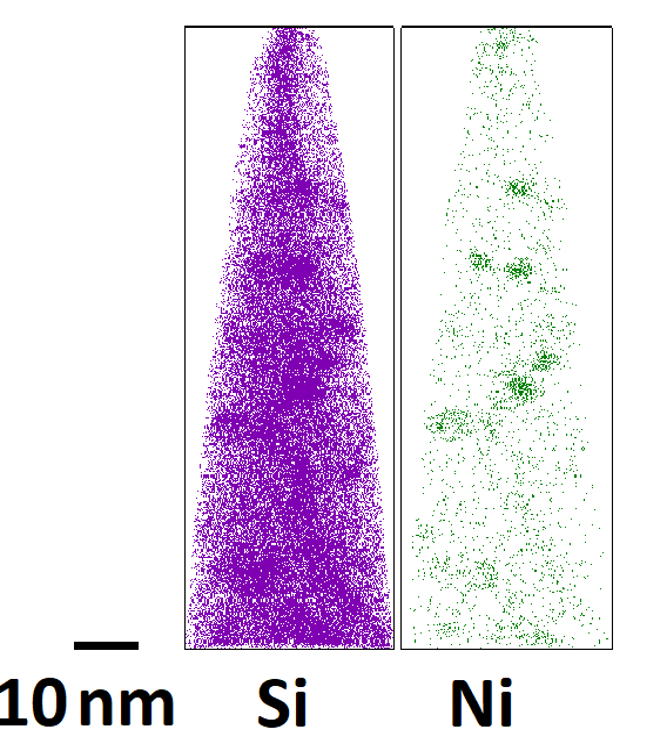
\includegraphics[scale=0.5]{APPLEvsATLAS_apple_EP} \\ а)
	\end{minipage}
	%\hfill
	\begin{minipage}[b][][b]{0.49\textwidth}\centering
		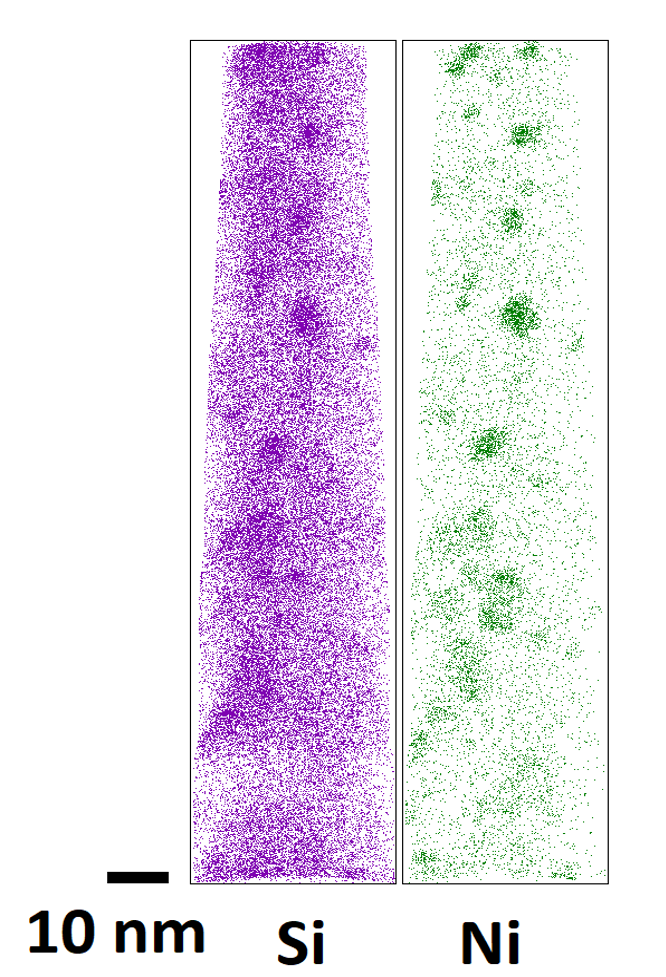
\includegraphics[scale=0.8]{APPLEvsATLAS_atlas_EP} \\ б)
	\end{minipage}
	\caption{Атомные карты облученной стали ЭП-823 на ПАЗЛ-3D (а) и АТЛАЗ (б).}
	\label{fig:APPLEvsATLAS_EP}
\end{figure} 

Поиск кластеров был проведен по Ni+ согласно алгоритму максимального разделения [ссылка на максимальное разделение]. Из пересечения соответствующих графиков, получены параметры идентификации кластеров по методу максимальной сепарации ($N_min$ = 7 и R = 8 для ПАЗЛ-3D и $N_min$ = 7 и R = 7.5 для АТЛАЗ). По найденным параметрам были выделены кластеры, после их отделения от матрицы. Были просмотрены кластеры на 3D изображении для выявления случайного объединения или выделения несоответствующий области в качестве кластера. Был создан отдельный масс-спектр для кластеров. В этом масс-спектре учитывались в приоритете элементы обогащения, в частности Ni++. Также внутри кластеров для обеих установок был обнаружен Nb и, соответственно, размечен. Данные масс-спектра отдельно матрицы и кластеров были экспортированы и объединены в общей таблице. В Таблицах \cref{tab:paramsAPPLEvsATLAS_EP3,tab:matrix_clustersAPPLEvsATLAS}, представлено сравнение данных для разных установок отдельно для стали ЭП-823.

\begin{table} [htbp]
	\centering
	\caption{Сравнения характеристик точности восстановления данных для ЭП-823 на установках ПАЗЛ-3D и АТЛАЗ}
	\label{tab:paramsAPPLEvsATLAS_EP3}
	\begin{SingleSpace}
		\begin{tabular} {| c | c | c |}
			\hline
			{}                                     & ПАЗЛ-3D & АТЛАЗ   \\ \hline
			$M/\Delta M_{50\%}$ Al$^+$             & 938     & 726     \\ \hline
			$M/\Delta M_{10\%}$ Al$^+$             & 245     & 329     \\ \hline
			Мульти-события, \%                     & 1.4     & 17.7                 \\ \hline
			Мульти-события Ni, \%                  & 1.7     & 28.6             \\ \hline
			Мульти-события Si, \%                  & 0.4     & 26.1             \\ \hline
			Мульти-события Cu, \%                  & 3.9     & 6.7             \\ \hline
			Шум, 10$^{-5}$ отн. ед.                & 10.05   & 30.1     \\ \hline
			Скорость сбора данных, атомов/возд.    & 0.008   & 0.01  \\ \hline
			Соотношение Al$^+$/Al$^{++}$, отн. ед. & 307     & 368     \\ \hline
		\end{tabular}
	\end{SingleSpace}
\end{table}

\begin{table} [htbp]
	\centering
	\caption{Сравнение состава матрицы [ат. \%] для алюминиевых сплавов Al-Cu-Mn-Zr после отжига при температурах 350 °С и 450 °С, полученных на установках ПАЗЛ-3D и АТЛАЗ}
	\label{tab:matrix_clustersAPPLEvsATLAS}
	\begin{SingleSpace}
		\begin{tabular} {| c | c | c | c | c |}
			\hline
			{} & \thead{ПАЗЛ-3D матрица} & \thead{АТЛАЗ матрица} & \thead{ПАЗЛ-3D кластеры} & \thead{АТЛАЗ кластеры} \\ \hline
			Fe       & 83.43 $\pm$ 0.02 & 83.98 $\pm$ 0.02  & 48 $\pm$ 1      & 53 $\pm$ 1  \\ \hline
			Cr       & 11.11 $\pm$ 0.06 & 10.51 $\pm$ 0.05  & 6.9 $\pm$ 0.8   & 7.3 $\pm$ 0.7   \\ \hline
			Si       & 2.59 $\pm$ 0.06  & 1.88 $\pm$ 0.05   & 15 $\pm$ 1      & 10.0 $\pm$ 0.8 \\ \hline
			Mn       & 0.94 $\pm$ 0.06  & 1.98 $\pm$ 0.05   & 4.5 $\pm$ 0,6   & 4.7 $\pm$ 0.5   \\ \hline
			Ni       & 0.59 $\pm$ 0.06  & 0.78 $\pm$ 0.05   & 23 $\pm$ 1      & 21 $\pm$ 1   \\ \hline
			Cu       & 0.05 $\pm$ 0.04  & 0.08 $\pm$ 0.05   & 0.2 $\pm$ 0,1   & 0.5 $\pm$ 0.2   \\ \hline
			W        & 0.16 $\pm$ 0.06  & 0.28 $\pm$ 0.05   & 0.03 $\pm$ 0,03 & 0.2 $\pm$ 0.1   \\ \hline
			C        & 0.08 $\pm$ 0.06  & 0.09 $\pm$ 0.05   & 0.11 $\pm$ 0,06 & 0.08 $\pm$ 0.06   \\ \hline
			Nb       & 0.07 $\pm$ 0.06  & -                 & 0.3 $\pm$ 0.1   & 0.5 $\pm$ 0.1   \\ \hline
			Остальные & Баланс & Баланс & Баланс & Баланс               \\ \hline			
		\end{tabular}
	\end{SingleSpace}
\end{table}


В Таблице \cref{tab:matrix_clustersAPPLEvsATLAS} представлено сравнение химического состава материалов как в кластерах, так и в матрице для стали ЭП-823. Средний размер кластеров на ПАЗЛ-3D составил (2.8 $\pm$ 0.2) нм, на АТЛАЗ средний размер равен (3.2 $\pm$ 0.4) нм. Рассчитана средняя плотность кластеров в объеме, которая составила (1.2 $\pm$ 0.4) x 10$^{23}$ и (1.1 $\pm$ 0.2) x 10$^{23}$ м$^3$ для ПАЗЛ-3D и АТЛАЗ соответственно.

Как видно из полученных выше характеристик точности восстановления данных установки ПАЗЛ-3D и АТЛАЗ сравнимы по разрешению по массе и для алюминиевых сплавов, и для сталей. Сравнение количества шума проводилось на участках масс-спектра после пиков основных элементов и сопоставлялось с учетом нормирования на общее число собранных атомов. Количество шума при исследовании алюминиевого сплава отличается в 3-6 раз в пользу АТЛАЗ, но в случае со сталью ситуация противоположная (на АТЛАЗ шума больше в три раза). Данный факт вызван скорее разными условиями испарения образцов – разная скорость сбора данных и неодинаковая форма образцов. Наблюдаются общие закономерности при сравнении доли мульти-событий. На АТЛАЗ детектируется существенно больше мульти-событий, чем на ПАЗЛ-3D. В случае исследования чистых материалов или алюминиевых сплавов это практически не играет роли. При исследовании стали получены данные с 17.7 \% мульти-событий. Предположительно, это может быть вызвано использованием криогенной системы без устройств гашения вибраций на АТЛАЗ (вибрации могут составлять более 20 мкм), на которую непосредственно закреплен держатель образца. Это может приводить к частому выходу образца из области освещения лучом лазера, что влечет за собой необходимость поддерживать более высокую интенсивность испарения в моменты корректного освещения вершины образца. Известно, что в этом случае количество мульти-событий возрастает, и снижается точность химической идентификации \cite{scbibOptParamsYAFI}. Различия в пропорции между элементами в мульти-событиях для алюминиевых сплавов, как видно из результатов, не вносит существенного различия в определяемый химический состав матрицы и кластеров. Скорее всего, отсутствие разницы обусловлено малым значением общего числа мульти-событий. Для ЭП-823, при исследовании на АТЛАЗ, получены существенно большие значения мульти-событий как для общее числа, так в пропорциях по элементам. Как следствие, наблюдаются отличия по концентрациям для Si, Mn, W и Cr, что, скорее всего, может быть нивелировано более точным подбором условий испарения или модернизацией прибора за счет уменьшения вибраций держателя образца.

Сравнение результатов исследования вольфрама позволяет заключить, что установки имеют практически идентичное пространственное разрешение 1-4 \r{A}. Это позволяет предположить, что все пространственные характеристики при сравнении данных должны быть иметь мало различий между установками. Данный тезис подтверждается при сравнении среднего размера кластеров в стали ЭП-823 и преципитатов Zr в алюминиевом сплаве. В обоих случаях средний размер нано-размерных объектов совпадает в пределах статистической погрешности. С другой стороны, в сплаве Al-Cu-Mn-Zr 350°С на разных установках наблюдается некоторое отличие рассчитанной плотности кластеров. Ввиду небольшой разницы результатов (всего в 1.5 раза) можно предположить, что причина отклонения в плотности частиц связана с реальными различиями плотности в разных зернах материала. При этом химический состав как матрицы, так и частиц для алюминиевых сплавов совпадает в пределах погрешности.

\FloatBarrier

\section{Методика коррекции восстановления атомно-зондовых данных с учетом атомной плотности}\label{sec:ch3/sect5}

Точность восстановления данных существенно зависит от параметров калибровки АЗТ и типа алгоритма восстановления. Трехмерные координаты вычисляются по известному принципу проекции. Можно использовать несколько алгоритмов восстановления координат. Основное различие между ними заключается в том, как они учитывают детали эволюции радиуса наконечника образца или координаты Z во время исследования APT \cite{Vurpillot16}. В наиболее распространенном алгоритме, предложенном Басом и др. \cite{Bas95}, предполагается, что радиус острия образца пропорционален напряжению. Этот алгоритм удобен для учета изменения формы образца и его радиуса. Однако это может быть неточно при анализе многофазного материала. Другой алгоритм, предложенный группами Blavette и Virpillot \cite{Vurpillot11,Gault11}, подходит для постоянного изменения угла зрения во время исследования АЗТ. Этот алгоритм хорошо подходит для восстановления распределения атомов в материалах с разными фазами. Однако он не работает, когда атомы фаз имеют значительно разные скорости испарения, и поэтому скорости изменения радиуса сильно различаются в разных фазах. Другой вариант состоит в том, что изменение радиуса может быть учтено с помощью его прямых измерений на изображении образца с помощью просвечивающей электронной микроскопии и электронного микроскопа \cite{Larson11}. Основными параметрами восстановления являются коэффициент сжатия изображения (ICF или $\xi$), длина полета иона, поле испарения для конкретного материала, коэффициент поля ($k_f$), атомный объем ($\Omega$), эффективность обнаружения и анализируемая область. Некоторые параметры, такие как эффективность обнаружения или анализируемая область, являются характеристиками АЗТ-устройства и не изменяются во время АЗТ-исследования. Однако другие параметры не постоянны. Например, ICF зависит от формы образца или электростатической системы \cite{Geiser09,Gipson08}. Для определения характера изменения этих параметров были проведены калибровочные исследования для различных типов АЗТ: ECOTAP \cite{Geiser09}, LAWATAP \cite{Renaud03}, LEAP 3000 \cite{Renaud06}. Также было проведено моделирование полевого испарения для определения зависимости параметров реконструкции от различных условий испарения \cite{Vurpillot11,Miller14,Hatzoglou19}. Следовательно, алгоритм трехмерной реконструкции, предложенный Басом и др., необходимо модифицировать. В методике восстановления АЗТ, основанной на алгоритме, предложенном Басом и др. \cite{Bas95}, радиус кривизны острия образца R определяется напряжением U, приложенным к образцу. Для восстановления поперечных координат (X, Y) атомов используется стереографическая проекция:

\begin{equation}
	\label{eq:equation3_1}
	X = R \sin{\phi}\sin{\theta}	
\end{equation}
\begin{equation}
	\label{eq:equation3_2}
	Y = R \cos{\phi}\sin{\theta}	
\end{equation}

где $\theta$ - полярный угол, $\phi$ - азимутальный угол. Согласно алгоритму Баса радиус R пропорционален напряжению U: 

\begin{equation}
	\label{eq:equation3_3}
	R = \frac{U}{E k_f}
\end{equation}

Следует отметить, что в алгоритме реконструкции Bas (стандартный протокол реконструкции) $k_f$ и поле испарения E остаются постоянными на протяжении всего исследования APT. Группой GPM \cite{Gault11_Loi} было показано, что постоянство $k_f$ приводит к неточной реконструкции морфологии фазовых включений и размеров всего исследуемого объема. Для решения этой проблемы были приняты различные подходы.
Loi и другие \cite{Loi13} смоделировали влияние параметров реконструкции на данные зонда AP с помощью коммерческого программного обеспечения LORENTZ 2D v9.0 \cite{Asi02}. Для испаряющей системы с локальным электродом обнаружена прямая связь между параметрами реконструкции и геометрией образца вблизи вершины.
В работах Gault \cite{Gault11_Loi} и Hatzoglou \cite{Hatzoglou19} были предложены различные подходы для определения параметров реконструкции: эмпирические измерения и сравнение реконструкций с использованием смоделированных и реальных данных.
В работе группы GPM \cite{Hatzoglou19} моделирование полевого испарения в рамках модели, предложенной Вурпиллотом и др. \cite{Vurpillot13}, использовалось для получения таблицы зависимостей $k_f$ и ICF от напряжения U, приложенного к образцу APT для испарение атомов. Зависимость $k_f$ носит экспоненциальный характер $k_f \propto \exp(U)$, а ICF пропорциональна кубическому корню из $k_f$. Результаты моделирования показали хорошее согласие с экспериментальными данными. Исходными параметрами были начальный радиус кривизны и угол раствора образца. Эти результаты не были применимы к установкам APT, разработанным в ИТЭФ, из-за отсутствия локального электрода и другой электростатической системы.
В данной статье предлагается подход к трехмерной реконструкции координат атомов, основанный на алгоритме Bas и функциях напряжения $k_f$ и ICF, откалиброванных с учетом соответствия восстановленной и реальной плотностей материала образца.

\begin{figure}[htb]
	\centerfloat{
		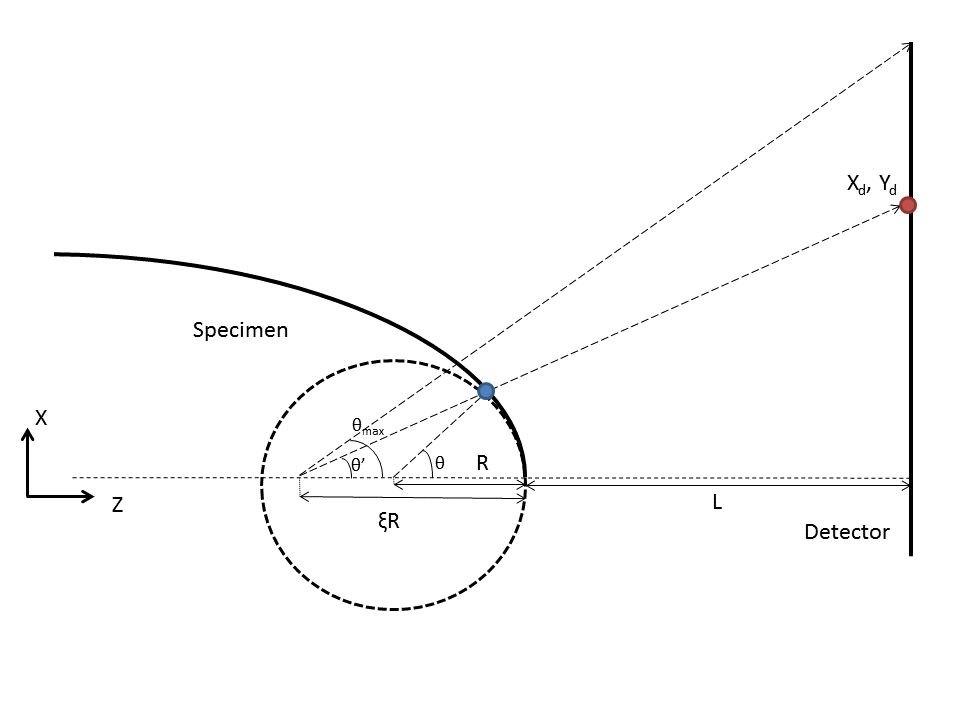
\includegraphics[width=\textwidth]{p3_projection}
	}
	\caption{Схематическое изображение точки-проекции: точка (X, Y) на наконечнике дает удар ($X_d$, $Y_d$). Определения углов в модели стереографической проекции.}
	\label{fig:p3_projection}
\end{figure} 
Координаты X и Y восстанавливаются с помощью стереографической проекции. Схема реконструкции представлена на Рисунке \cref{fig:p3_projection}. Прямая связь между двумя углами $\theta$ и $\theta$' и координатой Z может быть получена как:

\begin{equation}
	\label{eq:equation3_4}
	\theta = \theta' + \arcsin(\xi - 1)\sin{\theta'}
\end{equation}
\begin{equation}
	\label{eq:equation3_5}
	z_i = \frac{\Omega N_i}{Q R^2 \pi 2 {\sin^2(\theta_{max})}} + R (1- \cos{\theta})
\end{equation}

где $\theta$ - исходный угол запуска иона, который представляет собой реальный угол проекции, $\theta$' - угол, наблюдаемый после сжатия траекторий иона, Q - эффективность обнаружения, $N_i$ - номер обнаруженного атома. Угол $\theta_max$ - это максимальный угол обнаружения атомов. Уравнение \cref{eq:equation3_3} позволяет восстановить радиус в алгоритме Bas. Радиус впоследствии используется для восстановления координат. Важно отметить, что изменения kf играют важную роль в вычислении координаты Z, поскольку они влияют на значения обеих частей в сумме в \cref{eq:equation3_5}. Первая часть в \cref{eq:equation3_5} оказывает прямое влияние на координату Z. Второй (с ICF в $\theta$) - это поправка на кривизну поверхности. Следовательно, ICF влияет только на координаты X и Y. Чтобы продемонстрировать роль параметров реконструкции, одна и та же часть исследуемого образца была реконструирована с различными значениями $k_f$ и IFC (см. Рисунок \cref{fig:p3_3Dparts}). Как будет показано ниже, оптимальные значения $k_f$ и IFC могут быть выбраны, если реконструированная плотность материала образца приведена в соответствие с реальной.

\begin{figure}[htb]
	\centerfloat{
		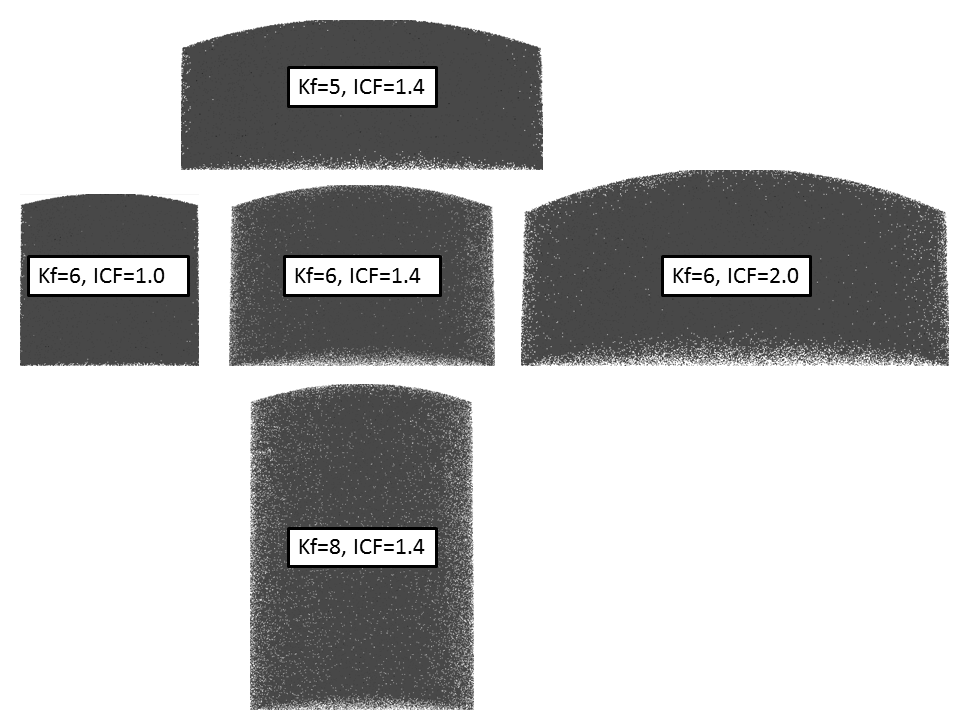
\includegraphics[width=\textwidth]{p3_3Dparts}
	}
	\caption{Карты атомов, построенные из одной и той же части исследуемого образца с различными параметрами $k_f$ и ICF}
	\label{fig:p3_3Dparts}
\end{figure}

\begin{figure}[htb]
	\begin{minipage}[b][][b]{0.49\textwidth}\centering
		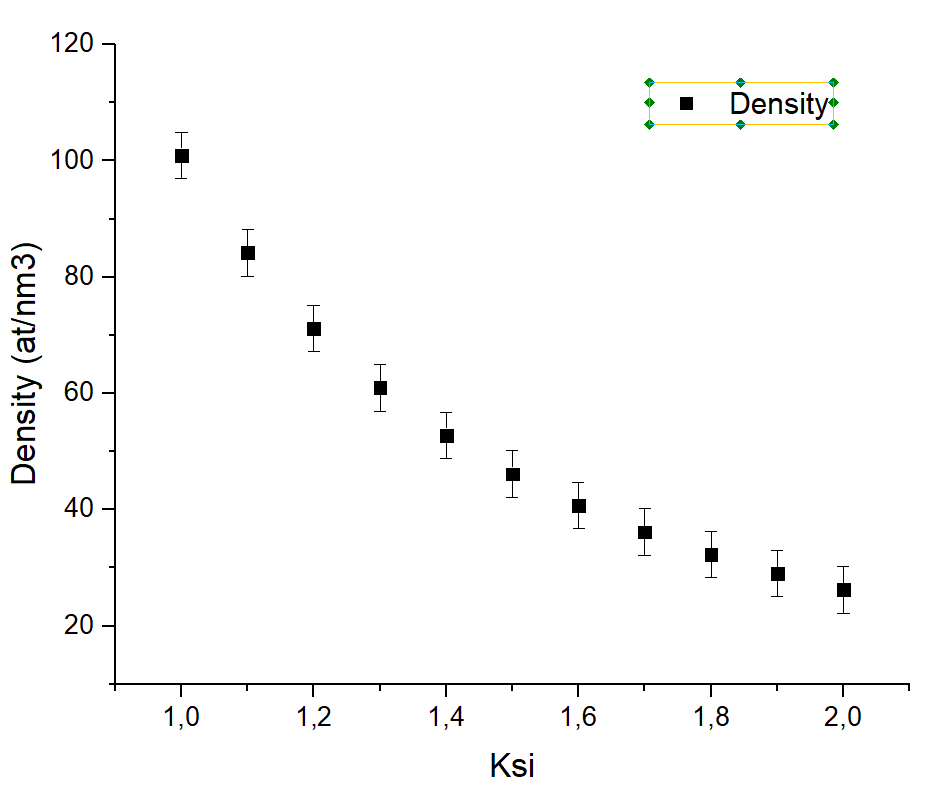
\includegraphics[width=\textwidth]{p3_ICFvsKsi} \\ а)
	\end{minipage}
	%\hfill
	\begin{minipage}[b][][b]{0.49\textwidth}\centering
		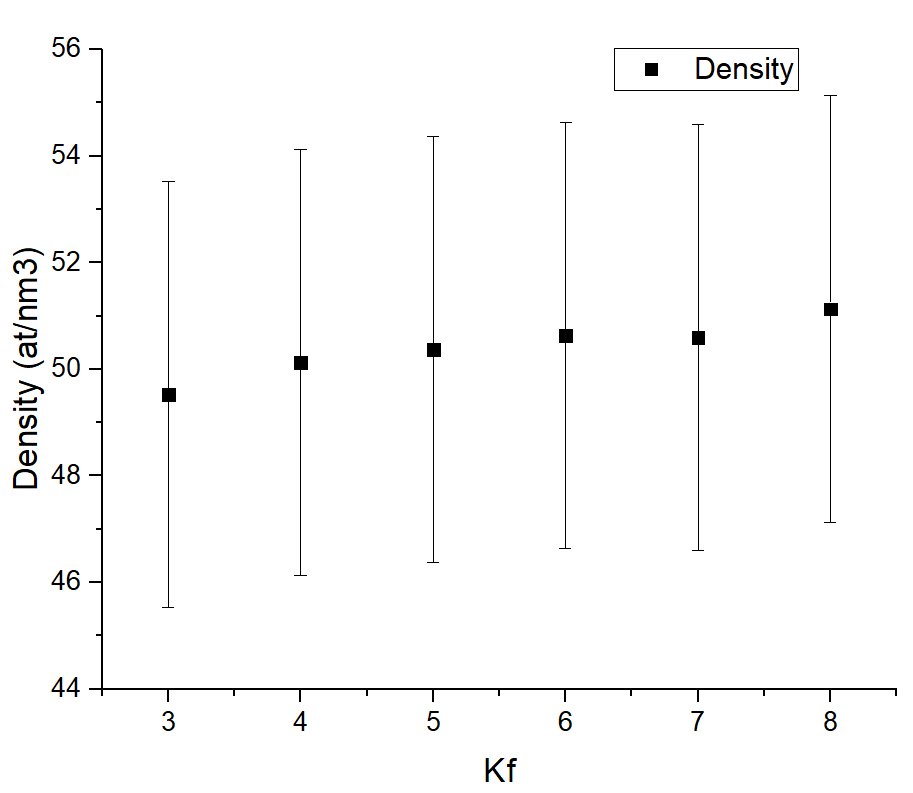
\includegraphics[width=\textwidth]{p3_ICFvskf} \\ б)
	\end{minipage}
	\caption{График атомной плотности как функции ICF (а). График атомной плотности как функции фактора поля $k_f$ (б)}
	\label{fig:p3_ICF}
\end{figure}

Следует отметить, что размер Z объема не изменяется при изменении ICF и фиксируется $k_f$, изменяются только радиус R и угол $\Theta$. Как объяснялось выше, это следствие выбранного алгоритма реконструкции. Как показано на Рисунке \cref{fig:p3_ICF} (б), атомная плотность не меняется с эволюцией $k_f$. Это связано с тем, что координаты X и Y пропорциональны радиусу, а Z обратно пропорциональна квадрату радиуса (см. Уравнения \cref{eq:equation3_1,eq:equation3_2,eq:equation3_5}). Таким образом, можно сделать вывод, что в алгоритме реконструкции $k_f$ и ICF можно откалибровать отдельно.
Принимая во внимание все перечисленные детали, предлагаем следующий алгоритм реконструкции. Первым шагом реконструкции является поиск динамического $k_f$. На значение $k_f$ напрямую влияет на все три координаты. Поэтому на данном этапе целесообразно использовать эмпирическую калибровку для восстановления кристаллических плоскостей. Второй шаг - это выбор динамического ICF, который практически не меняет расстояния в направлении Z. На этом этапе можно использовать плотность материала для определения правильной зависимости ICF. Мы предлагаем выбрать переменные параметры для согласования восстановленной плотности с реальной плотностью материала образца по всему объему.
Таким образом, при поиске ICF и $k_f$ используются известные значения, такие как межслоевые расстояния кристаллов и атомная плотность. Согласно работам групп Gault \cite{Gault11_Loi}, Loi \cite{Loi13} и Da Costa \cite{Hatzoglou19}, можно предположить, что зависимости ICF(U) и $k_f$(U), найденные для чистых материалов, будут одинаковыми по точности для сплавов.

Представленный АЗТ-анализ проводился на установке ПАЗЛ-3D в НИЦ Курчатовский институт - ИТЭФ \cite{scbibAPPLE}. В ПАЗЛ-3D используется лазерное полевое испарение, прямопролетная геометрия и программное обеспечение, разработанное в ИТЭФ. Образцы АЗТ получали электрохимическим методом с использованием стандартных электролитов. Форма кончика образцов контролировалась с помощью просвечивающего электронного микроскопа JEOL 1200 EX. В процессе сбора данных температура образца составляла 21 К, скорость сбора данных составляла от 2 до 6 атомов на 1000 лазерных импульсов, а энергия лазера составляла от 5 до 10 мВт с частотой 25 кГц. Для сплавов оптимальные условия испарения выбирались по методике, описанной в работе Разницына и др. \cite{scbibOptParamsYAFI}. Реконструкция данных проводилась с помощью программы КВАНТМ-3D \cite{KVANTM}. Для расчета масс-спектров с помощью этого программного обеспечения использовались процедуры автоматической калибровки и оптимизации \cite{Shutov19}.
Для восстановления массы и координат каждого атома использовалась программа КВАНТМ-3D. Для поиска зависимостей $k_f$(U) и ICF(U) были выбраны алюминий и вольфрам с гранецентрированной и объемноцентрированной кубической кристаллической структурой соответственно. Далее будут подробно описаны первый и второй этапы зависимостей поиска $k_f$(U) и ICF(U).

Как было написано выше, первым этапом алгоритма является поиск зависимости $k_f$ от напряжения на образце U. Объем образца разбивается на мелкие части по оси Z. Для каждой детали подбирается оптимальное расстояние между кристаллографическими плоскостями. Теоретические расстояния между атомными плоскостями соответствующих кристаллографических направлений взяты из приложения к книге Гаульта \cite{GaultBOOK}. Кристаллографические направления определялись по картам полевой десорбции. На Рисунке \cref{fig:p3_Alion} представлен пример карты полевой десорбции образца алюминия, полученной на АЗТ-детекторе.

\begin{figure}[htb]
	\centerfloat{
		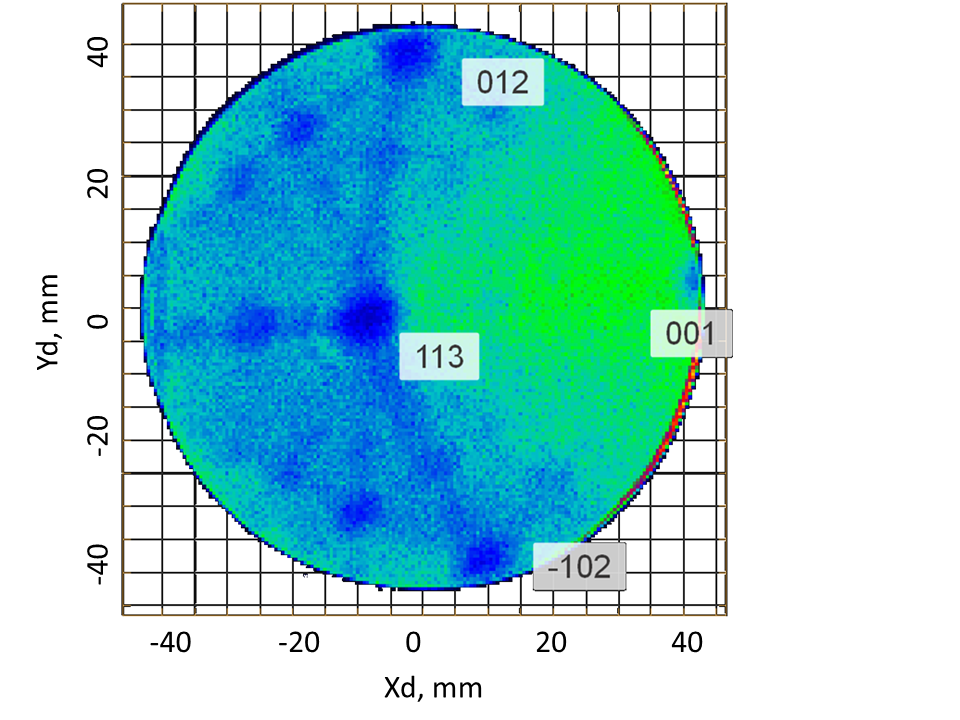
\includegraphics[width=\textwidth]{p3_Alion}
	}
	\caption{Карты полевой десорбции алюминиевого образца. Указаны кристаллографические направления}
	\label{fig:p3_Alion}
\end{figure} 

Для калибровки было выбрано ближайшее к центру детектора направление. Для большинства образцов этими направлениями были {111}, {001} и {113}. Информацию о межслоевых расстояниях, соответствующих выбранному направлению, можно взять из книги Гаульта \cite{GaultBOOK}. На Рисунке \cref{fig:p3_Alion} наиболее удобным направлением является {113} с расстоянием между атомными плоскостями около 1,2 \r{A}. Далее объем образца разбивался на мелкие части по оси Z. Каждая часть содержала 10-30 атомных плоскостей. Таким образом стало возможным найти значение $k_f$ для каждого небольшого кусочка образца. Напряжение на вершине в этих частях принималось постоянным для каждой из них. Полученные пары значений $k_f$ и напряжения U аппроксимировались функциональной зависимостью аналогичной в работе \cite{Hatzoglou19}. Пример аппроксимации данных выборки показан на Рисунке \cref{fig:p3_kf_vs_voltage}.

\begin{figure}[htb]
	\centerfloat{
		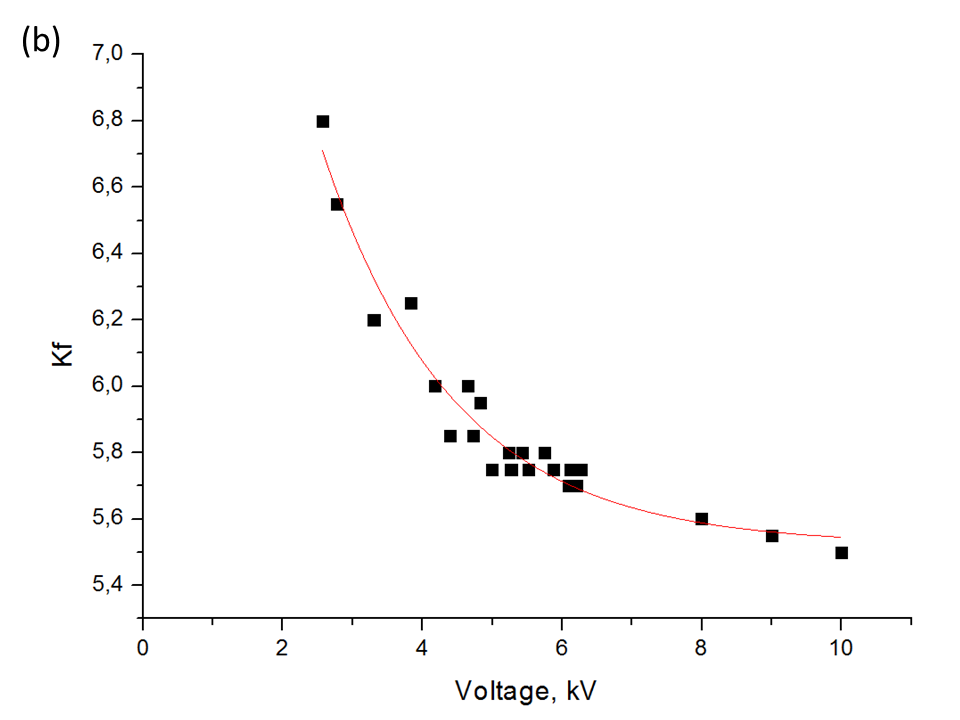
\includegraphics[width=\textwidth]{p3_kf_vs_voltage}
	}
	\caption{Экспериментальные данные $k_f$(черные точки) и наилучшая аппроксимирующая кривая (красная)}
	\label{fig:p3_kf_vs_voltage}
\end{figure} 

Описанная выше процедура была проведена для образцов из алюминия и вольфрама. $k_f$ как функция напряжения U была получена для каждой вершины. Из полученных данных была найдена общая зависимость $k_f$(U):

\begin{equation}
	\label{eq:equation3_6}
	k_f = (10 - C) + C\exp(- U * 5.3E-4)
\end{equation}

где C - константа подгонки. Значение постоянной зависит от состава материала. Например, для алюминия он равен 5,5, а для вольфрама - 4,5. Возможно, значение постоянной зависит от поля испарения материала. Явной разницы между коэффициентами в выражении \cref{eq:equation3_6} и углом стержня или начальным радиусом вершины не обнаружено. Полученная зависимость $k_f$(U) является экспоненциальной. Подобный характер зависимости был получен в работах Да Коста \cite{Hatzoglou19} и Лои \cite{Loi13}.
Следующим шагом после восстановления значения kf является корректировка значений ICF. Точность трехмерной реконструкции положения атомов в латеральном направлении недостаточна для идентификации кристаллической решетки. Согласно результатам, представленным на рис. 2, плотность может использоваться как критерий для получения значений ICF, обеспечивающих точность координат «сжатия» в плоскости XY. Тот же подход с разделением большого объема на мелкие части был использован для определения калибровочной кривой. Для каждой детали были найдены значение kf с использованием кристаллографических плоскостей и значение ICF с использованием плотности материала. Получена линейная зависимость ICF от напряжения на образце U. Зависимость ICF отличалась от полученных в аналогичных исследованиях \cite{Hatzoglou19, Gault11_Loi}. Это различие могло быть связано с режимом лазерного испарения в случае APPLE-3D в отличие от режима испарения с использованием локального электрода.
В программе анализа данных «КВАНТМ-3D» реализован инструмент «Линейная плотность» для построения графика атомной плотности вдоль выбранного направления. Атомная плотность рассчитывается вдоль выбранного направления. Для наглядности рисуется график с выбранным шагом. Примеры рассчитанных графиков плотности вдоль оси образца показаны на Рисунке \cref{fig:p3_Density_vs_depth} для алюминиевого образца с оптимизацией или без нее.

\begin{figure}[htb]
	\centerfloat{
		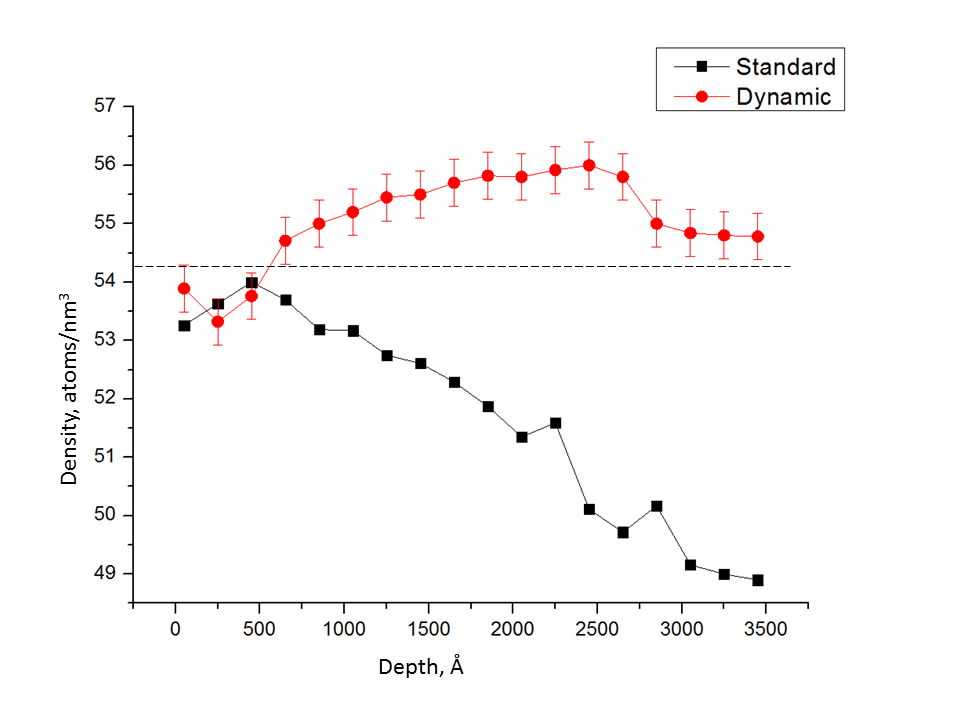
\includegraphics[width=\textwidth]{p3_Density_vs_depth}
	}
	\caption{Линейная атомная плотность вместе с образцом алюминия, полученная по стандартным протоколам и протоколам динамической реконструкции. Пунктирная линия показывает реальную плотность алюминия.}
	\label{fig:p3_Density_vs_depth}
\end{figure}

Необходимо скорректировать ожидаемую плотность для эффективности системы обнаружения для каждого прибора АЗТ, чтобы сравнить полученные значения с теоретическими. На использованной установке APPLE-3D установлена система детектирования с микроканальными пластинами с эффективностью детектирования ~ 90\%. В результате двух этапов калибровки были найдены динамические $k_f$ и ICF. Далее необходимо проверить эти зависимости на чистых материалах.

Предлагаемый протокол был протестирован на чистых материалах Al и W. Вольфрам имеет объемно-центрированную кубическую кристаллическую структуру с постоянной решетки около 3,16 \r{A} и 60,2 атома на кубический нанометр. Алюминий имеет гранецентрированную кубическую кристаллическую структуру с постоянной решетки около 4,05 \r{A} и 63,6 атома на кубический нанометр. Всего было исследовано 12 образцов алюминия и вольфрама. Для проверки точности реконструкции использовался специальный прибор для оценки расстояний между атомными плоскостями. Принцип этого инструмента основан на алгоритме распределения ближайших соседей k-го порядка \cite{GaultBOOK}. В программе КВАНТМ-3D этот инструмент называется «KNN-krist». Поиск соседей проводился только для атомов в выбранном направлении. Вместо дальнейшего поиска кластеров на гистограмму было нанесено распределение расстояний между ближайшими соседними атомами (см. Рисунок \cref{fig:p3_atomiccount_distance}). Расстояния между атомными плоскостями на разной глубине по оси Z были рассчитаны для всех образцов для стандартного и нового алгоритмов калибровки. Разница между этими алгоритмами показана на Рисунках \cref{fig:p3_PlanesDistance_depth,fig:p3_atomiccount_distance}.

\begin{figure}[htb]
	\centerfloat{
		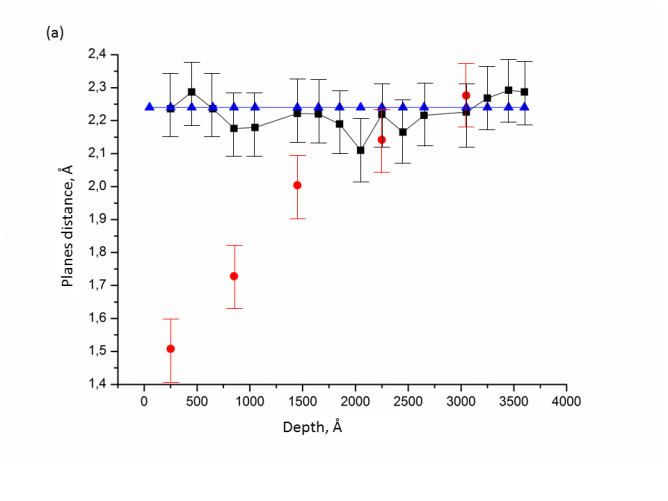
\includegraphics[width=\textwidth]{p3_PlanesDistance_depth}
	}
	\caption{Расстояние между атомными плоскостями как функция глубины по оси Z образца, полученное стандартным протоколом реконструкции (красный), динамическим протоколом $k_f$ и ICF (черный) и теоретическим значением (синий)}
	\label{fig:p3_PlanesDistance_depth}
\end{figure}
\begin{figure}[htb]
	\centerfloat{
		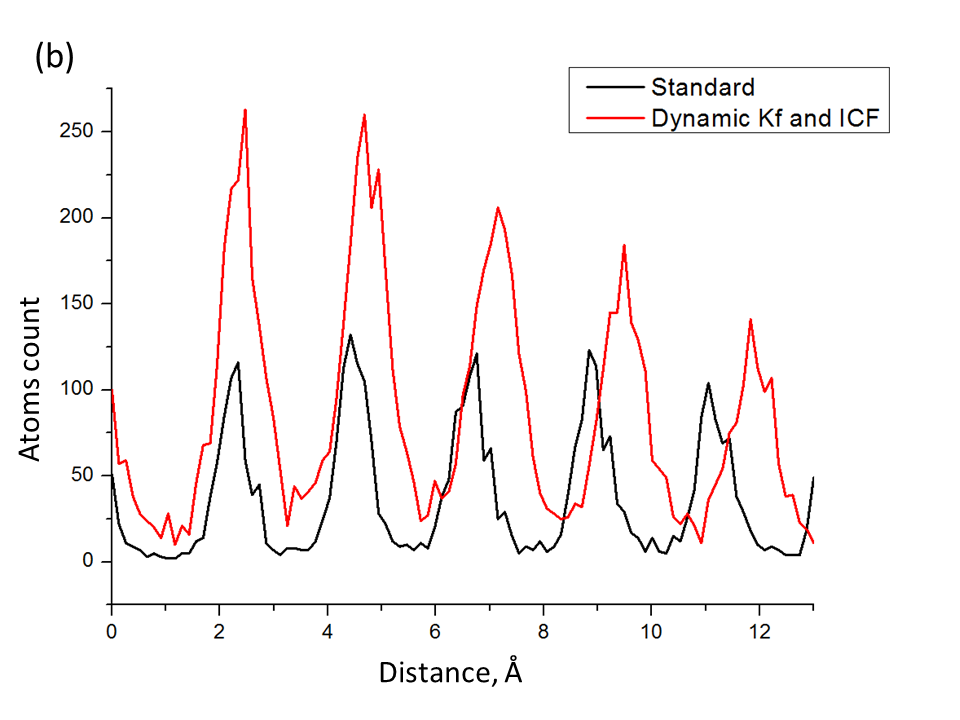
\includegraphics[width=\textwidth]{p3_atomiccount_distance}
	}
	\caption{Результат процедуры KNN-cryst для стандартных и динамических алгоритмов восстановления.}
	\label{fig:p3_atomiccount_distance}
\end{figure}

На Рисунке \cref{fig:p3_PlanesDistance_depth} видно, что ошибка в межплоскостных расстояниях, полученных в начале и в конце сбора данных АЗТ, может достигать 50\%. Важно отметить, что предлагаемые поправки могут значительно улучшить оценку размеров кластеров / фаз. Кроме того, учет этой поправки повлияет на точность расчета размеров переходных слоев, фаз и зерен. 
В этой статье был предложен алгоритм трехмерной реконструкции для данных АЗТ с использованием контроля плотности восстановленного материала. Этот протокол основан на алгоритме восстановления Баса. Отличительной особенностью этого протокола является проверка плотности материала вдоль выбранного направления для повышения точности восстановления данных. Динамические значения $k_f$ и ICF были измерены с использованием как кристаллографии, так и инструмента контроля плотности материала.

%\subsection{Подпараграф \cyrdash{} два}\label{subsec:ch3/sect33/sub2}

%Некоторый текст.














\clearpage
           % Глава 3
\chapter{Экспериментальные результаты}\label{ch:ch4}

\section{Апробация ПАЗЛ-3D для исследования алюминиевого сплава системы Al-Mg-Si}\label{sec:ch4/sect1}

В настоящее время установка ПАЗЛ-3D прошла широкую апробацию на различных материалах. Исследовались исходные состояния ферритно-мартенситных сталей ЭК-181, ЧС-139 [ref], дисперсно-упрочненных оксидами сталей ODS Eurofer, KP-(1-4), 10Cr ODS, 13.5Cr ODS, Austenitic ODS, ЭП-450 ДУО, ЭП-823 ДУО [ref], никелевые супер-сплавы [ref],  высокоэнтропийные сплавы [ref], и др. В настоящей главе представлены резульаты аппробации АЗТ установки ПАЗЛ-3D для сплавов алюминия, экономно-легированных сталей ЧТО-ТО ЕЩЁ.

Для тестирования установки были выбраны многокомпонентные сплавы с хорошей теплопроводностью, содержащие в своей структуре образования с характерным размером от единиц до сотен нанометров. Выбранный сплав Al-Mg-Si обладает повышенной прочностью, пластичностью, коррозийной стойкостью и жаростойкостью. Для выбранного сплава использовались следующие параметры исследования: температура образца 50~К, мощность лазерного излучения с гармоникой 515 нм составляла 10 мВт, скорость сбора данных в ходе эксперимента поддерживалась в пределах от 100 до 500 атомов/сек. Выбранные параметры являются наиболее часто используемыми для АЗТ исследований алюминиевых сплавов.

На Рисунке \cref{fig:AlMgSi_mass} представлена основная часть масс-спектра, полученного в результате проведения атомно-зондового исследования. Среднее разрешение по массе на полувысоте пиков составляет 500 отн. ед.

\begin{figure}[htb]
	\centerfloat{
		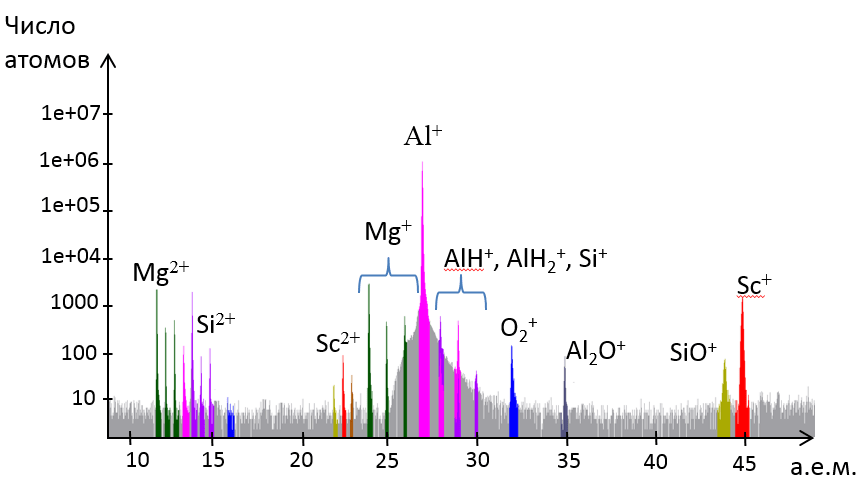
\includegraphics[width=.8\textwidth]{AlMgSi_mass}
	}
	\caption{Масс-спектр сплава Al-Mg-Sc (показана основная часть)\cite{scbibAlumYAFI}}
	\label{fig:AlMgSi_mass}
\end{figure} 
\FloatBarrier

На полученных атомных картах хорошо видны наноразмерные включения обогащенные Mg, Si, O и Cu. На Рисунке~\cref{fig:AlMgSi_3D}~(б) показаны атомные карты распределения Mg и Si. Включения Mg-Si имеют длину 50$\pm$10 нм и 10$\pm$2 диаметр. Поскольку включения имеют не сферическую форму, то для определения их концентраций использовались изо-концентрационные поверхности и проксиграммы. Химический состав матрицы и включений показан в Таблице \cref{tab:AlMgSi_table}. На Рисунке~\cref{fig:AlMgSi_3D}~(а) показаны изо-концентрационные поверхности Mg-Si 16~ат.~$\%$ (внутри таких поверхностей концентрация Mg-Si больше или равна 16~ат.~$\%$). Объемная плотность частиц составляет 2х$10^{22}$ см$^{-3}$.

\begin{figure}[htbp]
	\begin{minipage}[b][][b]{0.49\textwidth}\centering
		%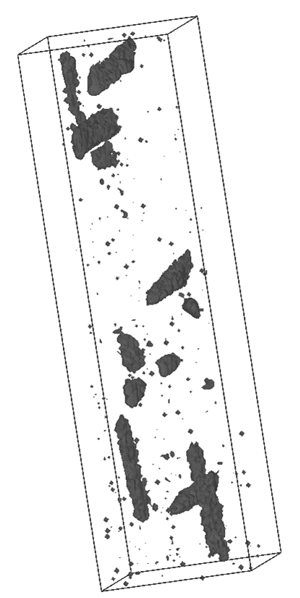
\includegraphics[width=\textwidth]{AlMgSi_3D_a} \\ а)
		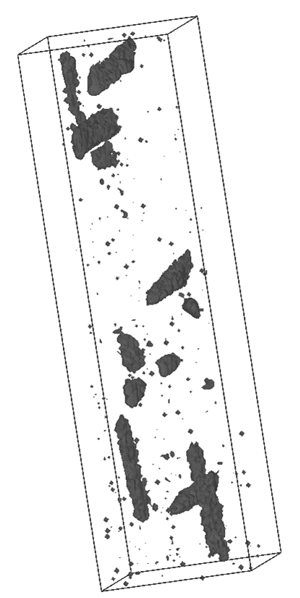
\includegraphics[scale=0.8]{AlMgSi_3D_a} \\ а)
	\end{minipage}
	%\hfill
	\begin{minipage}[b][][b]{0.49\textwidth}\centering
		%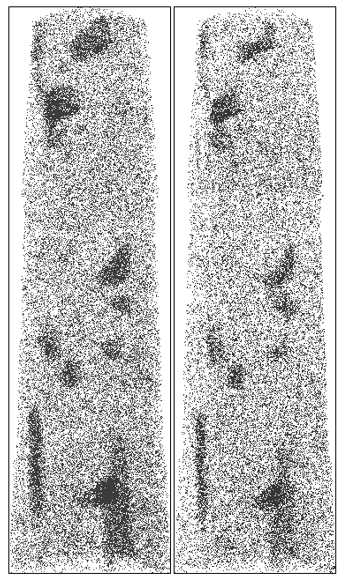
\includegraphics[width=\textwidth]{AlMgSi_3D_b} \\ б)
		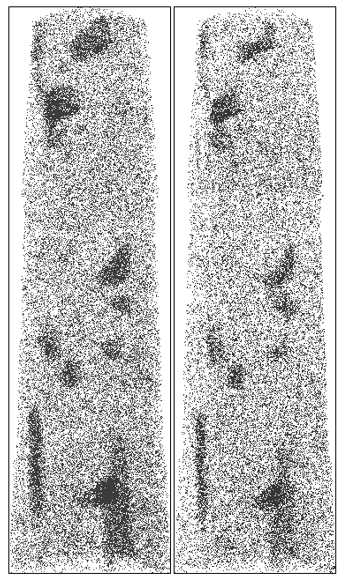
\includegraphics[scale=0.8]{AlMgSi_3D_b} \\ б)
	\end{minipage}
	\caption{а) Изоконцентрационные поверхности Mg и Si 16~ат.~$\%$, б) атомные карты распределения Mg (левый объем) и Si (правый объем). Размер исследованной области 47х47х167 нм$^3$}
	\label{fig:AlMgSi_3D}
\end{figure} 

\begin{table} [htbp]
	\centering
	%\begin{threeparttable}% выравнивание подписи по границам таблицы
	\caption{Состав матрицы и включений сплава Al-Mg-Si at. $\%$}%
	\label{tab:AlMgSi_table}%
	\begin{SingleSpace}
		\begin{tabular}{| c | c | c |}
			\hline
			Элемент & Матрица & Включения \\ \hline
			Al & 98.67 $\pm$ 0.01 & 67 $\pm$ 3 \\ \hline
			Mg & 0.56 $\pm$ 0.01 & 18 $\pm$ 3 \\ \hline
			Si & 0.35 $\pm$ 0.01 & 13 $\pm$ 2 \\ \hline						
			Cu & 0.03 $\pm$ 0.01 & 0.35 $\pm$ 0.03\\ \hline
			Остальные (O, S) & Баланс & Баланс \\ \hline			
		\end{tabular}%
	\end{SingleSpace}
	%\end{threeparttable}
\end{table}

Применение АЗТ для алюминиевого сплава типа Al-Mg-Si продемонстрирована возможность исследования с получение детальной информации о размерах и составе включений с характерным размером в десятки нанометров. Получены атомные карты распределений элементов в исследуемых объемах. Проведена оценка размеров и состава включений и матрицы материала.

\FloatBarrier

\section{Демонстрация возможности АЗТ по исследованию структуры среднеуглеродистой стали}\label{sec:ch4/sect2}

Для демонстрации возможностей АЗТ по исследованию промышленных высокопрочных износостойких сталей была выбрана среднеуглеррдистая сталь Б1700 (C 0.45, Si 0.36, Mn 1.13, Ni 0.67, Cu 0.63, Cr 1.26, Mo 0.40, Ti 0.03, V 0.06, Nb 0.02, Ca 0.03, B 0.003, S 0.008, P 0.005 масс.\%) в виде листового проката после отпуска при различных температурах. Основной целью было показать распределение углерода и легирующих элементов в объеме. В ходе исследований параметры работы установки поддерживались на следующих значениях: температура образца 40~К, мощность лазерного излучения гармоники 515~нм 1.5~мВт, скорость сбора данных от 60 до 500 атомов/сек.

Полученные атомные карты образца стали после отжига при 150 \textdegree С показаны на Рисунке \cref{fig:SteelAtomMaps1}, общий объем полученных данных составляет 23x23x200 нм$^{3}$. В Таблице \cref{tab:SteelComposition150} показан состав общий образца, состав матрицы и состав выделенных областей 1 и 2 на атомных картах.

\begin{figure}[ht]
	\centerfloat{
		\includegraphics[width=.7\textwidth]{SteelAtomMaps1}
	}
	\caption{Атомные карты образца среднеуглеродистой стали после отпуска при 150 \textdegree С \cite{scbibRyabov}. Состав областей 1 и 2 показан в Таблице \cref{tab:SteelComposition150} }
	\label{fig:SteelAtomMaps1}
\end{figure} 

\begin{table} [htbp]
	\centering
	\caption{Состав стали, исследованного образца, матрицы и областей 1 и 2 среднеуглеродистой стали после отпуска при температуре 150 \textdegree С (at.\%)}%
	\label{tab:SteelComposition150}%
	\begin{SingleSpace}
		\begin{tabular}{|p{3cm}| c | c | c | c | c | c | c | c | c | c | c |}
			\hline
			& C & Si & Mn & Ni & Cu & Cr & Mo & Ti & V & Nb & Al     \\ \hline
			Состав массивного образца     & 0.45 & 0.36 & 1.13 & 0.67 & 0.63 & 1.26 & 0.40 & 0.03 & 0.06 & 0.02 & 0.04   \\ \hline
			Среднее по объему   & 0.45 & 0.42 & 1.11 & 0.49 & 0.62 & 1.37 & 0.23 & - & 0.07 & 0.10 & 0.04   \\  \hline		
			Матрица   & 0.26 & 0.41 & 1.09 & 0.38 & 0.46 & 1.34 & 0.19 & - & 0.07 & 0.05 & 0.05   \\  \hline	
			Область 1   & 0.97 & 0.53 & 1.31 & 0.49 & 0.51 & 1.54 & 0.32 & - & 0.08 & 0.12 & 0.09   \\  \hline
			Область 2   & 0.71 & 0.28 & 1.12 & 0.94 & 1.05 & 1.34 & 0.38 & - & 0.07 & 0.32 & 0.04   \\  \hline	
		\end{tabular}%
	\end{SingleSpace}
\end{table}

Для анализа локального распределения элементов построен профиль линейных концентраций вдоль всего образца (Рисунок \cref{fig:SteelLinear1}). По линейным концентрациям и атомным картам можно явно определить наличие областей с повышенным содержанием углерода, оценить их морфологию и состав. Средняя концентрация углерода в углеродных включениях составляет 1.5~ат.\%. Присутствует также сегрегация углерода, дополнительно обогащенная также никелем, ниобием и молибденом.

\begin{figure}[ht]
	\centerfloat{
		\includegraphics[width=.8\textwidth]{SteelLinear1}
	}
	\caption{Линейные профили концентраций для образца среднеуглеродистой стали после отпуска при 150 \textdegree С \cite{scbibRyabov}}
	\label{fig:SteelLinear1}
\end{figure}

\begin{figure}[htb]
	\centerfloat{
		\includegraphics[width=.8\textwidth]{SteelAtomMaps2}
	}
	\caption{Атомные карты образца среднеуглеродистой стали после отпуска при 350 \textdegree С \cite{scbibRyabov}}
	\label{fig:SteelAtomMaps2}
\end{figure}

Для второго состояния материала (после отпуска при 350 \textdegree С) также получены атомные карты (Рисунок \cref{fig:SteelAtomMaps2}). Размер полученных данных составляет 25х25х100 нм$^{3}$. В Таблице \cref{tab:SteelComposition350} показан состав массивного образца и матрицы. Состав матрицы, без учета включений примерно соответствует составу массивного образца за исключением углерода, молибдена и ниобия. 

Для более детальной характериазции углеродного включения был построен отдельный линейный профиль концентрации для малого 3D объема (Рисунок \cref{fig:SteelLinear2}). На Рисунке \cref{fig:SteelAtomMapsLin} показана область, которая была выбрана для построения линейного профиля. Данный профиль наглядно демонстрирует обогащение углеродом границы зерна до 0.8~ат.\%, а также заметно обогащение по хрому и марганцу до 1.5~ат.\% каждый.

\begin{figure}[htb]
	\centerfloat{
		\includegraphics[width=.3\textwidth]{SteelAtomMapsLin}
	}
	\caption{Атомная карта распределения углерода образца среднеуглеродистой стали после отпуска при 350 \textdegree С \cite{scbibRyabov}. Показана область и направление построения линейной концентрации для границы зерна.}
	\label{fig:SteelAtomMapsLin}
\end{figure}

\begin{figure}[htb]
	\centerfloat{
		\includegraphics[width=.8\textwidth]{SteelLinear2}
	}
	\caption{Линейные профили концентраций для границы зерна образца среднеуглеродистой стали после отпуска при 350 \textdegree С \cite{scbibRyabov}}
	\label{fig:SteelLinear2}
\end{figure}

\begin{table} [htbp]
	\centering
	\caption{Состав стали, исследованного образца, матрицы и областей 1 и 2 среднеуглеродистой стали после отпуска при температуре 350 \textdegree С (at.\%)}%
	\label{tab:SteelComposition350}%
	\begin{SingleSpace}
		\begin{tabular}{|p{3cm}| c | c | c | c | c | c | c | c | c | c | c |}
			\hline
			& C & Si & Mn & Ni & Cu & Cr & Mo & Ti & V & Nb & Al     \\ \hline
			Состав массивного образца     & 0.45 & 0.36 & 1.13 & 0.67 & 0.63 & 1.26 & 0.40 & 0.03 & 0.06 & 0.02 & 0.04   \\ \hline
			Среднее по объему   & 0.37 & 0.41 & 1.16 & 0.61 & 0.57 & 1.37 & 0.23 & - & 0.07 & 0.10 & 0.05   \\  \hline		
			Матрица   & 0.37 & 0.40 & 1.14 & 0.60 & 0.55 & 1.35 & 0.22 & - & 0.07 & 0.10 & 0.05   \\  \hline		
		\end{tabular}%
	\end{SingleSpace}
\end{table}
\FloatBarrier
Исследования методом атомно-зондовой микроскопии позволили выявить многочисленные сегрегации атомов углерода в образце после отпуска при 150 \textdegree C. Полученные данные хорошо согласуются с данными просвечивающей электронной микроскопии: после отпуска при 150~\textdegree C наблюдались наиболее мелкие карбиды со средним размером 13~нм и объемной плотностью $2.2*10^{22} m^{-3}$ \cite{scbibRyabov}. Для состояния  с большей температурой отпуска 300 \textdegree C наблюдаются крупные частицы размером до 164–180~нм на границах реечного мартенсита и на границах исходных аустенитных зерен, где остаточный аустенит с объемной долей встречается и до 5\% \cite{scbibRyabov}.

\FloatBarrier

\section{Исследование изменения структуры высокопрочной экономнолегированной стали}\label{sec:ch4/sect3}

В качестве другого примера для апробации созданной установки ПАЗЛ-3D также были выбраны низкоуглеродистые стали. Одной из актуальных задач в разработке низкоугеродистых сталей является повышение уровня прочности и требуемой прокаливаемости при закалке \cite{scbibGlubev}. Данный класс материалов важен в разработке новых атомных ледоколов и морских технических средств добычи углеводородов. Для улучшения основных характеристик материала используются различные системы легирования. В процессе закалки или высокотемпературного отпуска может изменяться как микро, так и наноструктура материала. Соответственно, атомно-зондовая томография может предоставлять важную информацию о локальном распределении химических элементов в данных материала на различных этапах обработки.

Для демонстрации возможности АЗТ исследований использовалась сталь 09ХГН2МД. Состав стали мас. \%: 0.090 С; 0.30 Si; 0.70 Mn; 3.0 (Cr+Ni+Cu+Mo); 0.027 (V+Nb); 0.04 Al; 0.004 Ti; 0.002 Sn; 0.006 N; 0.003 S; 0.007 P. Были изучены три состояния,  состав образца и кластеров (при их наличии) показан в Таблице~\cref{tab:SteelComposition09X}. Исследование проводилось при следующих условиях: температура образца 40~К, мощность лазерного излучения при гармонике 515~нм 1.6~мВт, скорость сбора данных от 60 до 250 атомов/сек.

%\begin{itemize}
%	\item Закалка от 950 \textdegree C
%	\item Закалка от 950 \textdegree C + отпуск при 570 \textdegree С
%	\item Закалка от 950 \textdegree C + отпуск при 630 \textdegree С
%\end{itemize}

\begin{table} [htbp]
	\centering
	\caption{Состав образцов и кластеров для 09ХГН2МД (средние значения), ат.\%}
	\label{tab:SteelComposition09X}%
	\begin{SingleSpace}
		\begin{tabular}{| p{4.5cm} | c | c | c | c | c | c | c | c |}
			\hline
			 & & C & Si & Mn & Ni & Cr & Mo & Nb     \\ \hline
			\multirow{2}{*}{Закалка от 950 \textdegree C} & Образец & 0.19 & 0.53 & 0.71 & 0.85 & 0.59 & 0.13 & 0.01    \\ \cline{2-9}
			& Кластеры & 3.38 & 0.60 & 0.79 & 0.77 & 0.44 & 0.17 & 0.02    \\  \hline		
			Закалка от 950 \textdegree C + отпуск при 570 \textdegree С & Образец & 0.06 & 0.57 & 0.72 & 0.97 & 0.52 & 0.13 & 0.006    \\ \hline
			\multirow{2}{45mm}{Закалка от 950 \textdegree C + отпуск при 630 \textdegree С} & Образец & 0.09 & 0.54 & 0.70 & 1.08 & 0.50 & 0.18 & 0.007    \\ \cline{2-9}
			& Кластеры & 3.88 & 0.59 & 1.00 & 1.25 & 0.74 & 0.71 & -    \\  \hline	
		\end{tabular}%
	\end{SingleSpace}
\end{table}

\FloatBarrier
С помощью АЗТ показано, что в закаленном состоянии наблюдаются кластеры (наночастицы с повышенным содержание углерода), в которых содержание основных легирующих элементов практически не отличается от матрицы. Но после отпуска при температуре 570 \textdegree С в течении 3 часов происходит диссоциация кластеров. После отпуска при температуре 630 \textdegree С с помощью АЗТ были обнаружены кластеры с повышенным содержанием C, Mn, Cr и Mo (см. Таблицу \cref{tab:SteelComposition09X}). Наблюдаемые с помощью АЗТ эффекты подтверждены с помощью ПЭМ исследований \cite{scbibGlubev}.

В данном исследовании методика АЗТ помогла установить особенности изменения структуры стали 09ХГН2МД при высокотемпературном отпуске. Полученные данные могут быть применены в задаче оптимизации режимов термической обработки листового проката.

\FloatBarrier

\section{Исследование алюминия МИСиС Торгом}\label{sec:ch4/sect4}

Ожидает согласования с МИСиС Торгом

\FloatBarrier
\clearpage
\section{Основные результаты по главе 4}\label{sec:ch4/sect5}


В главе показаны возможности АЗТ установки ПАЗЛ-3D по исследованию материалов с нано-размерными особенностями. Продемонстрированы примеры визуализации АЗТ данных с помощью таких инструментов как: масс-спектры, атомные карты, линейные профили концентраций, изо-концентрационные поверхности и поиск кластеров. Продемонстрированный набор инструментов позволяет достаточно полно и подробно описывать кластеры/фазы в исследуемых материалах.

На примере исследования алюминиевого сплава типа Al-Mg-Si показана возможность изучения состава и структуры зон Гинье-Престона. Размер исследуемых зон может быть от нескольких нанометров до нескольких десятков нанометров. Также показана возможность программного обеспечения по визуализации нано-размерных объектов с помощью изо-концентрационных поверхностей.

Также в главе показаны исследования среднеуглеродистой стали Б1700. С помощью атомных карт показано распределение углерода в объеме образцов. Построены линейные профили концентраций химических элементов. Рассчитана объемная плотность карбидов в материале.


В рамках исследования высокопрочной экономнолегированной стали 09ХГН2МД показана возможность проводить поиск кластеров с определением их состава.




\FloatBarrier
\clearpage











%\nopagebreak - не разрывать страницами?







           % Глава 4
\chapter*{Заключение}                       % Заголовок
\addcontentsline{toc}{chapter}{Заключение}  % Добавляем его в оглавление

%% Согласно ГОСТ Р 7.0.11-2011:
%% 5.3.3 В заключении диссертации излагают итоги выполненного исследования, рекомендации, перспективы дальнейшей разработки темы.
%% 9.2.3 В заключении автореферата диссертации излагают итоги данного исследования, рекомендации и перспективы дальнейшей разработки темы.
%% Поэтому имеет смысл сделать эту часть общей и загрузить из одного файла в автореферат и в диссертацию:

Основные результаты работы заключаются в следующем:
%% Согласно ГОСТ Р 7.0.11-2011:
%% 5.3.3 В заключении диссертации излагают итоги выполненного исследования, рекомендации, перспективы дальнейшей разработки темы.
%% 9.2.3 В заключении автореферата диссертации излагают итоги данного исследования, рекомендации и перспективы дальнейшей разработки темы.
\begin{enumerate}[beginpenalty=10000]
	\item Впервые в России создана установка атомно-зондовой томографии с фемтосекундным лазерным испарением, позволяющая проводить атомно-зондовые исследования широкого спектра материалов  и получать информацию о трехмерном распределении элементов в объеме образца с разрешением, близким к атомному. Пространственное разрешение установки составляет не хуже 4 \r{A}. Разрешение по массе на полувысоте на ПАЗЛ-3D в среднем находится в диапазоне от 500 до 600~отн.~ед. (в зависимости от материала и условий исследований).
	\item Проведена первичная оценка необходимой мощности лазерного излучения для испарения образцов в атомно-зондовом томографе ПАЗЛ-3D. Требуемая мощность равна 13 $\pm$ 6 мВт. Выбрана оптимальная поляризация пучка (90\textdegree относительно предустановленной в лазерной системе) для более эффективного испарения.
	\item Разработана оригинальная методика коррекции атомно-зондовых данных по атомной плотности материала для компенсации ошибки восстановления трехмерных координат. Данная методика обеспечивает восстановление 3D координат атомов точнее на 50~\%, чем стандартные алгоритмы обработки для длины исследуемого объема более 300 нм.   
	\item Разработана методика контроля условий испарения для разных атомно-зондовых томографах с использованием метрики соотношения зарядностей одно- и двухзарядных пиков основного химического элемента материала образца. Сравнение результатов исследований алюминиевого сплава и стали показало, что отклонение ключевых характеристик находится в пределах погрешности или допустимых отклонений для данных материалов. Данная методика позволит улучшит повторяемость результатов исследований.	
	\item В результате проведения исследований набора сплавов изучены возможности установки по исследованию материалов с нано-размерными особенностями. Показаны способы обработки и представления результатов исследований, такие как: поиск кластеров, масс-спектр, атомные карты, профили концентраций, анализ состава материала, изо-концентрационные поверхности.  Проведены демонстрационные исследования состава и структуры ряда сплавов с помощью атомно-зондовой томографии:
	\begin{itemize}
		\item Получены атомные карты химических элементов для сплава Al-Mg-Si. Измерены плотность и характерные размеры включений Mg-Si. Получен состав нано-размерных включений.
		\item Исследованы сегрегации атомов углерода(кластеры) и крупные карбидные частицы в образцах среднеуглеродистой стали после различных температур отпуска.
		\item Подтверждено наличие кластеров углерода в экономнолегированной стали при высокотемпературном отпуске
		\item Продемонстрированы возможности изучения профилей концентраций для когерентных и полу-когерентных границ $\theta '$-фазы на примере сплава Al-Si-Cu-Sn.
	\end{itemize}
\end{enumerate}


%И какая-нибудь заключающая фраза.
\clearpage
Благодарности:
\begin{itemize}
	\item С.В. Рогожкин - руководитель, наставник, конструктивная критика
	\item А.А. Алеев - наставник
	\item Шутов А.С., Разницын О.А. - помогали, критика
	\item Корчуганова, Никитин, Орлов, Искандаров - общая помощь
	\item остальные коллеги
\end{itemize}



      % Заключение
%\printnomenclature[3.5cm] % Значение ширины столбца с обозначениями стоит подбирать вручную
\chapter*{Список сокращений и условных обозначений}   
\addcontentsline{toc}{chapter}{Список сокращений и условных обозначений}  % Добавляем его в оглавление
\printnomenclature        % Список сокращений и условных обозначений
\include{Dissertation/dictionary}      % Словарь терминов
\include{Dissertation/references}      % Список литературы
\include{Dissertation/lists}           % Списки таблиц и изображений (иллюстративный материал)

\setcounter{totalchapter}{\value{chapter}} % Подсчёт количества глав

%%% Настройки для приложений
\appendix
% Оформление заголовков приложений ближе к ГОСТ:
\setlength{\midchapskip}{20pt}
\renewcommand*{\afterchapternum}{\par\nobreak\vskip \midchapskip}
\renewcommand\thechapter{\Asbuk{chapter}} % Чтобы приложения русскими буквами нумеровались




\chapter{Расчет разрешения по массе для различных длин пролета ионов для атомно-зондового томографа}\label{app:A}


\begin{longtable} {| p{3cm} | c | c | c | p{2cm} |}
	\caption{Сравнение разрешения по массе для иона при различных ускоряющих напряжениях на образце}\\
	\hline
	\textbf{\thead{Длина \\пролета, мм}} & \textbf{\thead{Разброс времени\\ пролета, нс}} & \textbf{\thead{Напряжение,\\ кВ}} & \textbf{\thead{Разрешение \\по массе, отн. ед.}} & \textbf{\thead{$\delta M/n$,\\ отн. ед.}} \\
	\hline
	\endfirsthead
	\multicolumn{5}{c}%
	{\tablename\ \thetable\ -- \textit{Начало на предыдущей странице}} \\
	\hline
	\textbf{\thead{Длина \\пролета, мм}} & \textbf{\thead{Разброс времени\\ пролета, нс}} & \textbf{\thead{Напряжение,\\ кВ}} & \textbf{\thead{Разрешение \\по массе, отн. ед.}} & \textbf{\thead{$\delta M/n$,\\ отн. ед.}} \\
	\hline
	\endhead
	\hline \multicolumn{5}{r}{\textit{Продолжение на следующей странице}} \\
	\endfoot
	\hline
	\endlastfoot
	%\hline
	%Длина пролета, мм & \thead{Разброс времени\\ пролета, нс} & Напряжение, кВ & \thead{Разрешение \\по массе, отн. ед.}  \\ \hline
	200 & 1 & 1  &  623 & 0.02             \\ \hline
	200 & 1 & 3  &  360 & 0.04            \\ \hline
	200 & 1 & 5  &  278 & 0.05            \\ \hline
	200 & 1 & 10 &  197 & 0.07             \\ \hline
	200 & 0.5 & 1  &  1246 & 0.01             \\ \hline
	200 & 0.5 & 3  &  719  & 0.02            \\ \hline
	200 & 0.5 & 5  &  557  & 0.03            \\ \hline
	200 & 0.5 & 10 &  394  & 0.04            \\ \hline
	195 & 1 & 1  &  607    & 0.01          \\ \hline
	195 & 1 & 3  &  351    & 0.04          \\ \hline
	195 & 1 & 5  &  271    & 0.05          \\ \hline
	195 & 1 & 10 &  192    & 0.08          \\ \hline
	195 & 0.5 & 1  &  1215   & 0.01          \\ \hline
	195 & 0.5 & 3  &  702    & 0.02          \\ \hline
	195 & 0.5 & 5  &  543    & 0.03          \\ \hline
	195 & 0.5 & 10 &  384    & 0.04          \\ \hline
	190 & 1 & 1  &  592  & 0.02            \\ \hline
	190 & 1 & 3  &  342  & 0.04            \\ \hline
	190 & 1 & 5  &  264  & 0.06            \\ \hline
	190 & 1 & 10 &  187  & 0.08            \\ \hline
	190 & 0.5 & 1  &  1184 & 0.01            \\ \hline
	190 & 0.5 & 3  &  684  & 0.02            \\ \hline
	190 & 0.5 & 5  &  529  & 0.03            \\ \hline
	190 & 0.5 & 10 &  374  & 0.04            \\ \hline
	185 & 1 & 1  &  576    & 0.03          \\ \hline
	185 & 1 & 3  &  333    & 0.04          \\ \hline
	185 & 1 & 5  &  258    & 0.06          \\ \hline
	185 & 1 & 10 &  182    & 0.08          \\ \hline
	185 & 0.5 & 1  &  1153 & 0.01             \\ \hline
	185 & 0.5 & 3  &  666  & 0.02            \\ \hline
	185 & 0.5 & 5  &  515  & 0.03            \\ \hline
	185 & 0.5 & 10 &  364  & 0.04            \\ \hline
	180 & 1 & 1  &  561    & 0.03          \\ \hline
	180 & 1 & 3  &  324    & 0.05          \\ \hline
	180 & 1 & 5  &  251    & 0.06          \\ \hline
	180 & 1 & 10 &  177    & 0.08          \\ \hline
	180 & 0.5 & 1  &  1122 & 0.01             \\ \hline
	180 & 0.5 & 3  &  648  & 0.02            \\ \hline
	180 & 0.5 & 5  &  501  & 0.03            \\ \hline
	180 & 0.5 & 10 &  354  & 0.04            \\ \hline
	175 & 1 & 1  &  545    & 0.03          \\ \hline
	175 & 1 & 3  &  315    & 0.05          \\ \hline
	175 & 1 & 5  &  244    & 0.06          \\ \hline
	175 & 1 & 10 &  172    & 0.09          \\ \hline
	175 & 0.5 & 1  &  1091 & 0.01             \\ \hline
	175 & 0.5 & 3  &  630  & 0.02            \\ \hline
	175 & 0.5 & 5  &  488  & 0.03            \\ \hline
	175 & 0.5 & 10 &  345  & 0.04            \\ \hline
	170 & 1 & 1  &  530    & 0.03          \\ \hline
	170 & 1 & 3  &  306    & 0.05          \\ \hline
	170 & 1 & 5  &  237    & 0.06          \\ \hline
	170 & 1 & 10 &  167    & 0.09          \\ \hline
	170 & 0.5 & 1  &  1059 & 0.01             \\ \hline
	170 & 0.5 & 3  &  612  & 0.02            \\ \hline
	170 & 0.5 & 5  &  474  & 0.03            \\ \hline
	170 & 0.5 & 10 &  335  & 0.05            \\ \hline
\end{longtable}


\begin{landscape}
\chapter{Параметры исследования сплава Al-3.5Cu-0.2Mn-0.1S}\label{app:B}


\begin{longtable}{|p{6cm}|c|c|c|c|c|c|c|c|c|}
	\caption{Метрики качества атомно-зондовых данных}\\
	\hline
	\textbf{Номер набора данных} & \textbf{1} & \textbf{2} & \textbf{3} & \textbf{4} & \textbf{5} & \textbf{6} & \textbf{7}& \textbf{8} & \textbf{9}\\
	\hline
	\endfirsthead
	\multicolumn{10}{c}%
	{\tablename\ \thetable\ -- \textit{Начало на предыдущей странице}} \\
	\hline
	\textbf{Номер набора данных} & \textbf{1} & \textbf{2} & \textbf{3} & \textbf{4} & \textbf{5} & \textbf{6} & \textbf{7}& \textbf{8} & \textbf{9} \\
	\hline
	\endhead
	\hline \multicolumn{10}{r}{\textit{Продолжение на следующей странице}} \\
	\endfoot
	\hline
	\endlastfoot
	Мощность, отн. ед. & 400 & 500 & 600 & 700 & 800 & 900 & 1000 & 500 & 600  \\ \hline
	Однократные события, \% & 97.06 & 97.79 & 98.41 & 97.14 & 94.48 & 95.56 & 96.48 & 94.93 & 97.36              \\ \hline
	Доля мультисобытий Cu, \% & 4.12 & 3.66 & 4.36 & 2.72 & 2.89 & 2.94 & 3.11 & 2.78 & 3.24     \\ \hline
	Поток событий, атомов/1000 воздействий    & 0.0045 & 0.0045 & 0.0035 & 0.0055 & 0.0085 & 0.008 & 0.007 & 0.004 & 0.0055      \\ \hline
	Напряжение, кВ  & 5.0-5.7 & 4.2-4.9 & 3.2-4.2 & 5.8-7.1 & 7.4-7.8 & 7.8-8.5 & 8.5-9.0 & 9.6-9.9 & 5.5-5.8        \\ \hline
	Шум, \%         & 14 & 8.5 & 6 & 20 & 15 & 17 & 21 & 42 & 11       \\ \hline
	Шум на промежутке 10-11 а.е.м., отн. ед.    & 100 & 40 & 18 & 54 & 49 & 56 & 61 & 213 & 45      \\ \hline
	Шум на промежутке 40-41 а.е.м., отн. ед.    & 135 & 65 & 24 & 100 & 124 & 156 & 210 & 495 & 83   \\ \hline
	Концентрация Cu, \%    & 0.53 & 0.70 & 0.89 & 0.77 & 0.88 & 0.85 & 0.91 & 0.59 & 0.75   \\ \hline
	Концентрация Sn, \%    & - & 0.02 & 0.01 & 0.01 & - & <0.01 & <0.01 & - & -    \\ \hline
	Концентрация Mn, \%    & - & 0.006 & 0.01 & 0.006 & - & - & 0.005 & - & -    \\ \hline
	Соотношение Al$^+$/Al$^{++}$, отн. ед., \%    & 78 & 170 & 386 & 210 & 182 & 230 & 289 & 73 & 168    \\ \hline
	Число атомов (0-100 а.е.м.)    & \thead{514 748} & \thead{558 408} & \thead{591 629} & \thead{4 538 007} & \thead{2 648 840} & \thead{5 898 660} & \thead{7 653 641} & \thead{1 899 266} & \thead{581 324}      \\ \hline
\end{longtable}

%\clearpage

\begin{longtable} {| p{6cm} | c | c | c | c | c | c | c | c | c |}
	\caption{Метрики качества атомно-зондовых данных}\\
	\hline
	\textbf{Номер набора данных} & \textbf{1} & \textbf{2} & \textbf{3} & \textbf{4} & \textbf{5} & \textbf{6} & \textbf{7}& \textbf{8} & \textbf{9}\\
	\hline
	\endfirsthead
	\multicolumn{10}{c}%
	{\tablename\ \thetable\ -- \textit{Начало на предыдущей странице}} \\
	\hline
	\textbf{Номер набора данных} & \textbf{1} & \textbf{2} & \textbf{3} & \textbf{4} & \textbf{5} & \textbf{6} & \textbf{7}& \textbf{8} & \textbf{9} \\
	\hline
	\endhead
	\hline \multicolumn{10}{r}{\textit{Продолжение на следующей странице}} \\
	\endfoot
	\hline
	\endlastfoot
		Мощность, отн. ед. & 80 & 100 & 110 & 130 & 130 & 110 & 150 & 150 & 170  \\ \hline
		Однократные события, \% & 97.35 & 96.70 & 96.43 & 97.45 & 96.13 & 97.26 & 97.19 & 96.78 & 97.29              \\ \hline
		Доля мультисобытий Cu, \% & 3.13 & 3.07 & 2.66 & 3.80 & 2.35 & 3.43 & 3.07 & 3.02 & 3.25               \\ \hline
		Шум, \%         & 14 & 8.5 & 6 & 20 & 15 & 17 & 21 & 42 & 11               \\ \hline
		Шум на промежутке 10-11 а.е.м., отн. ед.    & 100 & 40 & 18 & 54 & 49 & 56 & 61 & 213 & 45      \\ \hline
		Шум на промежутке 40-41 а.е.м., отн. ед.    & 135 & 65 & 24 & 100 & 124 & 156 & 210 & 495 & 83      \\ \hline
		Концентрация Cu, \%    & 0.53 & 0.70 & 0.89 & 0.77 & 0.88 & 0.85 & 0.91 & 0.59 & 0.75      \\ \hline
		Концентрация Sn, \%    & - & 0.02 & 0.01 & 0.01 & - & <0.01 & <0.01 & - & -      \\ \hline
		Концентрация Mn, \%    & - & 0.006 & 0.01 & 0.006 & - & - & 0.005 & - & -      \\ \hline
		Соотношение Al$^+$/Al$^{++}$, отн. ед., \%    & 78 & 170 & 386 & 210 & 182 & 230 & 289 & 73 & 168      \\ \hline
		Число атомов (0-100 а.е.м.)    & \thead{514 748} & \thead{558 408} & \thead{591 629} & \thead{4 538 007} & \thead{2 648 840} & \thead{5 898 660} & \thead{7 653 641} & \thead{1 899 266} & \thead{581 324}      \\ \hline
\end{longtable}
\end{landscape}





\clearpage
\refstepcounter{chapter}        % Приложения

\setcounter{totalappendix}{\value{chapter}} % Подсчёт количества приложений

\end{document}
